

\let\cleardoublepage\clearpage

\chapter{Social Media Data Acquisition}

In this chapter we describe how we filtered for relevant tweets using two different lexicons. The food lexicon contains keywords with food related terms  (e.g. \emph {rice, wheat, milk}) where the predictor lexicon contains terms with factors influencing the price and supply of the goods (e.g. \emph{pricey}, \emph {cheap}, \emph{available}). We downloaded 2 TB of tweets from the internet archive \footnote{https://archive.org/details/archiveteam-json-twitterstream}  over a span of October 2011 - September 2014.  The filtering process resulted with 29 M food relevant tweets.

Firstly we motivate and detail an algorithm Hyperspace Analogue to Language (HAL)  \cite{lund96} for candidate term selection. We then  experimentally evaluate the  different metrics influencing the performance of HAL, discuss different frameworks for selecting candidate terms for our food, respectively predictor lexicon and lastly explain the filtering process of the tweets. 



\section{Hyperspace Analogue to Language}

HAL creates a semantic space from word co-occurrences \cite{lund96}. By using a sliding window parsing mechanism, the frequency of each term co-occurring within a fixed window size is recorded.  It is important to note that HAL only records the terms before the word we wish to analyse the context from. The terms after the word will appear in the column in the matrix that corresponds to that word.  The matrix is created by storing a vector for each word with the number of co-occurrences of every other word in the corpus. Hence, if our corpus contains $N$ different words the resulting HAL space would be a $N \times N$ square matrix of co-occurrences. Every time a specific word appears within the fixed window size the co-occurrence vectors are updated. For each co-occurrence HAL applies a scoring function. Words that appear closer, receive an inversely proportional score to its distance.

 To illustrate the idea \cite{burgess98} gives an example of a simple sentence \emph {The horse raced past the barn fell.} in Table \ref{tab:halex} with a sliding window of five. Let's consider the first row.  \emph{The} precedes \emph{Barn} twice. Once within a distance of five and the other time it directly precedes the word  \emph{Barn}. Hence, that cell receives a score of five for the proximate one and a score of one for the word further away resulting in a final score of six. 

Following the creation of the matrix we concatenate both the column and row vector of a word, where the former represents the preceding words and the later the following. To compare the distance of the vectors we used the cosine similarity function. 


\begin{table}[H]
\centering
\begin{tabular}{ c c c c c c} \toprule
  & Barn & Horse &  Past & Raced & The \\ 
  \hline
 Barn &  & 2 &  4 & 3 & 6 \\ 
 Fell & 5 & 1 &  3 & 2 & 4 \\ 
 Horse &  &  &   &  & 5 \\ 
 Past &  & 4 &   & 5 & 3 \\ 
 Raced &  & 5 &   &  & 4 \\ 
 The &  & 3 &  5 & 4 & 2 \\ 
   \bottomrule
\end{tabular}
\caption{Toy example of HAL}
\label{tab:halex}
\end{table}





\subsection{Motivating a Semantic Approach}
\label{subsec:hal}

HAL allows us to study the relationship between words. More specifically it's an algorithm that aids our goal of understanding what words are represented in the context of \emph{food} and topics centered around \emph{food security}. To achieve this target we need a methodology for representing the meaning of a word. We analyse the context of a word to identify new words that have a similar meaning or given an identical context express the same thing. The later is concerned with identifying synonyms where as the former looks at contextual similarity. For example, let us look at the word \emph {mold} and \emph {available}. Those two words seem unrelate, but given the context of food they express the same thing.  Namely an abundance of food. Through the context they posses elements of items similarity but by themselves they would never be considered words with similar meaning. It is important to stress that they are not similar because they occur frequently locally, but because they occur frequently in similar sentential context. Burgess et al. \cite{burgess98} argues that a simple local co-occurrence analysis misses to capture a lot of relationships. For example the word street and road are basically synonyms, however the seldom locally co-occur. They do however occur in the same context. This observation motivated us to deviate from the commonly used co-occurrence analysis and take a step further to improve the precision of our filtering framework. 







 











\subsection{Experimental Evaluation}
\label{sec:exp_eval}

To increase the recall of HAL we evaluated the performance on three different sample sizes (10 \%, 20 \%, 40 \%) constituting a corpus of around 23M, 47M, 93M words respectively. Our corpus of food related tweets has a number of appealing properties as it covers a large vocabulary centered around food. Unlike most corpora that represent formal reports or specialized dictionaries our food corpus represents everyday speech. This gives us a closer approximation on how people would talk in the context of our predictor categories. 

The initial set of words in our corpus was filtered only to contain those words that appear at least 100 times. Words occurring infrequent were discarded as well as stop words and punctuations. On a test sample of 10 \% we observed that around 10 \% of the tweets contain equal or less than four words which could impact the quality of the results. Hence, on the 40 \% sample we further excluded tweets that contain less or equal to four terms. Using the words $w \in F_c$ we produced a $N \times N$ matrix with the co-occurrences for three different window sizes namely five, eight and ten to investigate if the window size has an impact on the result. According to \cite{lund96} a window size of eight should yield the best results. However, the nature of a tweet is very different from a classical text so it remains to see if this observation holds for microblogs. Since vector similarity measures are sensitive to the magnitude of the vectors we normalized all the vectors to a constant length. 

\subsection{HAL Performance Results}


In Figure \ref{fig:price_supply} and Figure \ref{fig:poverty_needs} we can observe that for all categories HAL performed best with a window size of 10 which contradicts the findings of \cite{lund96}. Additionally, we see that the smaller sample sizes consistently produce more relevant keywords than the larger sample sizes.  A larger sample sizes increases the likelihood of a keyword's occurrence. Since we set a fixed threshold of 100 occurrences across all samples we are more likely to include words with a smaller confidence , which might explain the poor performance. 


\begin{figure}[H]
        \centering
        \begin{subfigure}[b]{0.5\textwidth}
                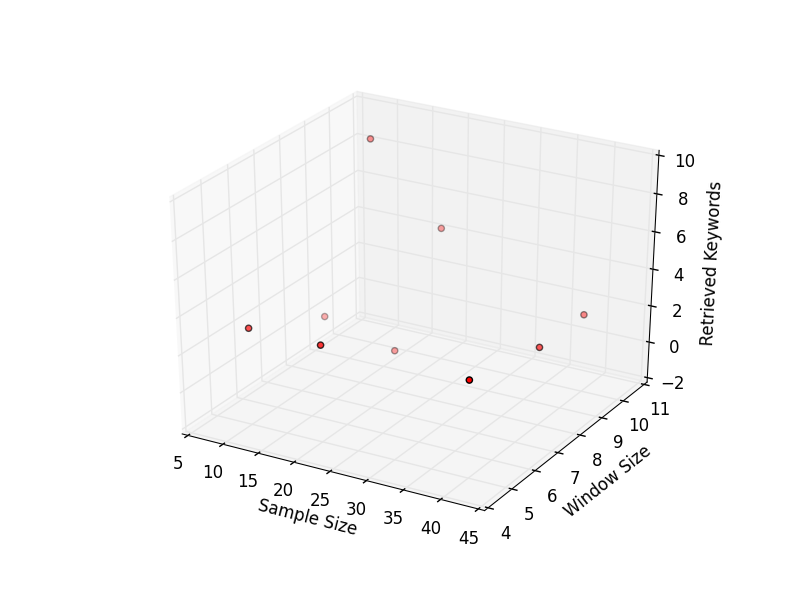
\includegraphics[width=\textwidth]{img/lex/price_hal}
                \caption{HAL - Price}
                \label{fig:al_price}
        \end{subfigure}%
        ~ %add desired spacing between images, e. g. ~, \quad, \qquad, \hfill etc.
          %(or a blank line to force the subfigure onto a new line)
        \begin{subfigure}[b]{0.5\textwidth}
                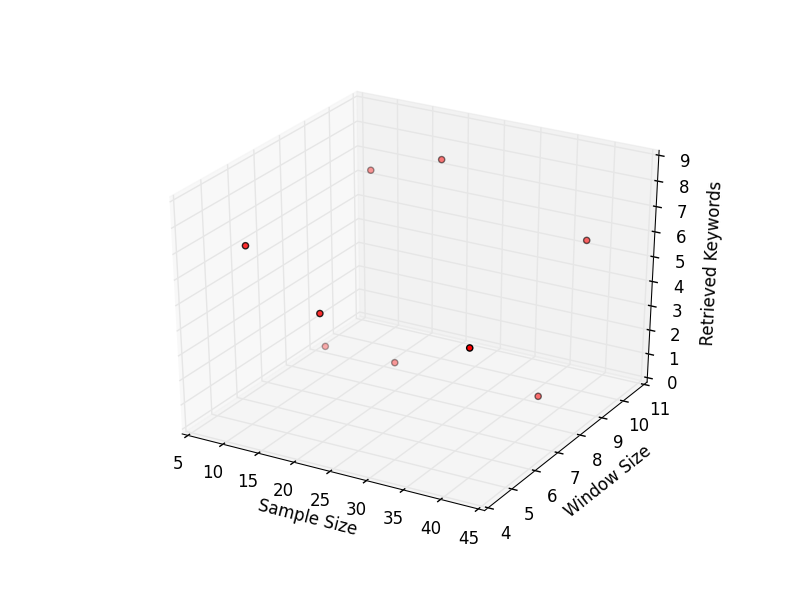
\includegraphics[width=\textwidth]{img/lex/supply_hal}
                \caption{HAL - Supply}
                \label{fig:hal_supply}
        \end{subfigure}
        ~ %add desired spacing between images, e. g. ~, \quad, \qquad, \hfill etc.
          %(or a blank line to force the subfigure onto a new line)
      
        \caption{HAL Evaluation for Price and Supply}\label{fig:price_supply}
\end{figure}


\begin{figure}[H]
        \centering
        \begin{subfigure}[b]{0.5\textwidth}
                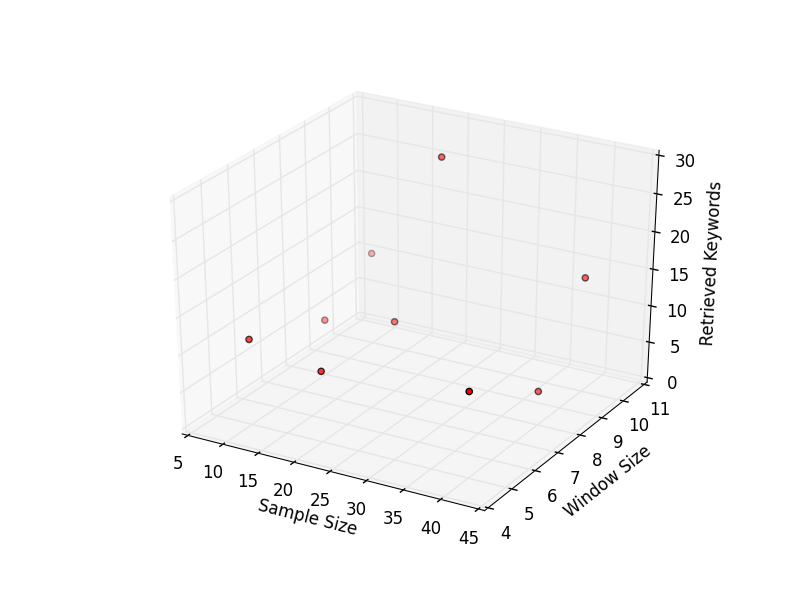
\includegraphics[width=\textwidth]{img/lex/needs_hal}
                \caption{HAL - Needs}
                \label{fig:al_price}
        \end{subfigure}%
        ~ %add desired spacing between images, e. g. ~, \quad, \qquad, \hfill etc.
          %(or a blank line to force the subfigure onto a new line)
       \begin{subfigure}[b]{0.5\textwidth}
                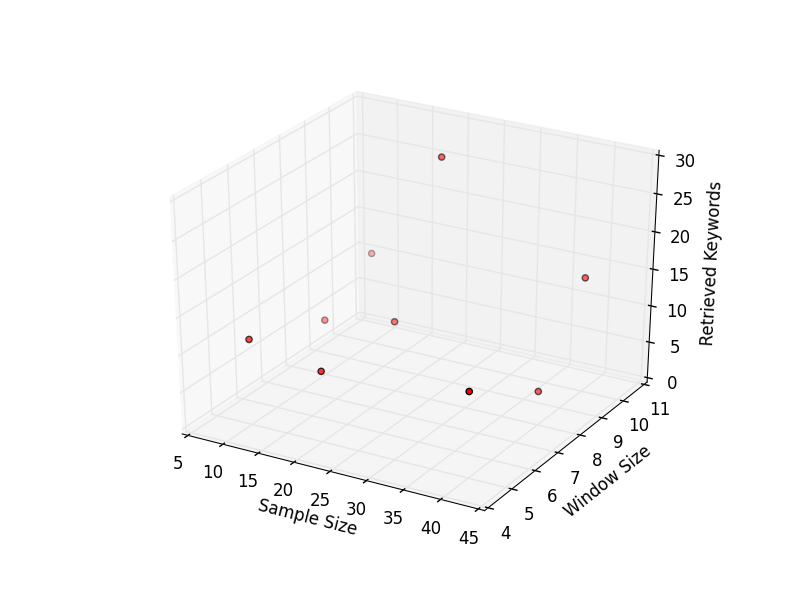
\includegraphics[width=\textwidth]{img/lex/needs_hal}
                \caption{HAL - Poverty}
                \label{fig:al_price}
        \end{subfigure}%
        ~ %add desired spacing between images, e. g. ~, \quad, \qquad, \hfill etc.
          %(or a blank line to force the subfigure onto a new line)
      
        \caption{HAL Evaluation for Poverty and Needs}\label{fig:poverty_needs}
\end{figure}

 
\subsection{Discussion}

We observed that HAL has a good precision given a high similarity threshold. For the top 20 keywords we evaluated a precision of 100 \% for food relevant terms. In the top 20 we found other food items building the majority of the retrieved words. However, the precision varies with the window and sample size. These variables, as our evaluation has shown, are very much dependent on the form of the corpus.  

With decreasing similarity HAL highlighted some topics indirectly associated with food security. For example there was a high percentage of country names that showed a clear association with food. Where the majority of the retrieved countries such as Thailand, Bali \footnote{http://www.nomad4ever.com/2008/08/24/top-10-popular-foods-of-asia-explained/} or the cities Singapore and Paris \footnote{http://www.hellotravel.com/stories/best-food-cities-in-world} are considered to be famous holiday destinations for food lovers other retrieved countries such as Pakistan, Syria, Jakarta India or the Philippines \footnote{http://foodsecurityindex.eiu.com/Country} are cities with a history of food insecurity and political unrest. 





\section{Food Lexicon}
\label{food_lex}

We began the construction of our Food Lexicon by considering  a simple list of food related keywords. To avoid ambiguities we will refer to the initial list of keywords as $K_{initial}$. Words included are the most common traded food commodities as listed by IMF \footnote{http://www.imf.org/external/np/res/commod/index.aspx} along the ten most important staple foods that feed the world \footnote{http://knowledge.allianz.com/demography/health/?767/the-worlds-staple-foods}. 

We filtered the archive dataset using exact string matching on $K_{initial}$. The distribution of the food related tweets motivated us to structure our lexicon hierarchically as certain commodities were only represented very sparsely and insufficient for further analysis. Where global keywords such as \emph{food} are highly represented, more specific keywords such as \emph{beef} occur infrequently. To circumvent this problem we mimic the hierarchical representation of the FAO   \footnote{http://www.fao.org/worldfoodsituation/foodpricesindex/en/}. 

FAO tries to measure the overall food fluctuation by five different food categories namely \emph{meat, dairy products, cereals, vegetable oil} and \emph {sugar}. We further created a category named \emph{Other Food of Interest}. This category contains general keywords (e.g. \emph{food, dinner or lunch}) and food keywords that cannot be assigned to one of the five categories, but frequently occur (e.g. \emph {coffee, tea}). To be considered frequent,  the set of tweets containing the keyword needs to be $> 1\%$ of the total sample. \emph{meat, dairy, cereals, vegetable oil} and \emph{other food of interest} build the top layer of our hierarchical representation as shown in Figure \ref{fig:food_lex}. 

For the second layer we use subcategories. As the name implies  subcategories abstract the categories into different subsets i.e. for meat we would have the subsets \emph{beef, chicken, lamb} and \emph{pork}. 

As the third layer and lowest instance, we consider food products. Each subcategory consists of food items which \textbf{1.)} can simply be the name of a category and subcategory (e.g. \emph{meat, beef}) or  \textbf{2.)} be a product that is commonly found in markets and stores around the world. An example of the later would be \emph{flour} for the subcategory \emph{wheat}. The intuition and motivation to include such products is simple. In the production process of food items most factors that influence the price are static and predictable. The only fluctuating and unknown factor is the price of the raw product or in our case the commodity. Products should hence be just as expressive in explaining the variance of food prices. One however has to be cautious as certain producers hedge themselves against price fluctuations of commodities allowing them to sell the product to the same price despite rising commodity prices. Lastly, we were motivated to include such terms because products are more likely to capture the social attention then raw items due to their every day use. 

\begin{figure}[H]

\Tree[.{FoodLexicon} [.{Meat} [.Beef \textit{Steak} ]
               [.Pork  \textit{Ham}  ] ]
          [.Dairy [.Cheese \textit{Mozzarella} ]
                [.Milk \textit{Cream}  ]]
                [.Cereals [.Wheat \textit{Flour} ]
                [.Corn  \textit{Whisky}  ]     ]]

\caption{Food Lexicon - Hierarchy}\label{fig:food_lex}
\end{figure}


 Other than the sparsity of the data we further faced the problem of ambiguous keywords. \emph {soy} is such a keyword that refers in English to the \emph{bean} and in Spanish to the verb \emph{to be}. To avoid such ambiguity we extended the term to make it distinct (e.g. \emph{soy} $\to$  \emph{soy bean}). Terms were added to the lexicon by following a framework as explained in the following section. 



\subsection{Candidate Food Term Selection}

We initially assume an empty set $K_{final}$ and structure it hierarchically as mentioned in the previous section. The six categories ($c_1, c_2 ... c_6)$ are $\in K_{final}$ where $c_i$ is one of the six categories mentioned above. For interpretability purposes we introduce an axiom in form of a set $K_{all}$. It only contains five of the above mentioned six categories \emph{meat, dairy products, cereals, vegetable oil, sugar} excluding the category \emph{other food of interest}. We assume that $K_{all}$ is a fully populated Lexicon containing all possible food items for a specific category (e.g. the subset dairy would contain all possible dairy products). It returns $True$ if a term is an element of the set and $False$ otherwise. For all keywords $k_i \in K_{initial}$ we evaluate if $k_i\in K_{all}$. If $True$ we consider $k_i \in K_{final}$. For all keywords $k_i \notin K_{all}$ the condition of it being frequent is evaluated and if $True$ added to the category \emph{0ther food of interest}  $c_6 \in K_{final}$.  Food commodities that could not be assigned to any of the six categories were discarded (e.g. \emph {orange, cocoa, onion}). Lastly, the set $K_{final}$  was further enriched by using food products $p_i$ that have been identified by \cite{AbbarMW14}  only if $p_i$ $\in K_{all}$ . To further improve our coverage of the six food categories we filtered for synonyms and contextual similar words using HAL. 

We summarize our framework as follows: 

\begin{description}
  \item[1.)] Add all keywords $k \in K_{initial}$ to  $K_{final}$ only if $k \in K_{all} $ or $k$ is frequent 
  \item[2.)] Include all $p_i$ to $K_{final}$ only if $p_i \in K_{all}$
  \item[3.)] Create a HAL space using a random subsample of 10\% from $K_{initial}$ with all keywords that occur $> 100$. $\forall c_i \in K_{final} $  pick the keyword $k\in K_{final}$ that most frequently occurs over the entire sample and retrieve the top 500 similar terms. Hand select those that are $\in K_{all}$ and add it to $K_{final}$.
\end{description}
 
The keyword set $K_{final}$ was used to perform exact term matching on the tweets collected from the internet archive. The resulting set of keywords in $K_{final}$ forms our Food Lexicon.  

 
\begin{table}[H]   
\centering
\scriptsize 
\begin{tabular}{p{1.3cm}|p{10.7cm} rlr}\toprule
\pbox{1.3cm}{Lexicon / \\ Subset $s$\\} & Keywords (i: from initial set, e: from \cite{AbbarMW14} , h: from HAL space )  \\
\hline
& & \\
\pbox{1.3cm}{$K_i$ \\Food } & \pbox{10.7cm}{  meal (i), meals (i) ,food (i), foods (i), wheat (i), rice v, maize (i), carley (i), soybean (i), soy (i), meat (i) , beef (i), cattle (i), chicken (i), poultry (i), lamb (i), swine (i), pork (i), fish (i), seafood (i), shrimp (i), salmon (i), sugar (i), bananas (i), oranges (i), coffee (i), cocoa (i), tea (i), milk (i), yams (i), cassava (i), potatoes (i), sorghum (i), plantain (i), nuts (i), onion (i), salt (i), egg (i), dairy (i), cereals (i)  }    \\
& & \\
 

\hline
\hline

& & \\
\pbox{1.3cm}{$K_f$ \\ Meat }  & \pbox{10.7cm}{ meat (i), lamb (i), pork (i), swine (i), chicken (i), poultry (i), beef (i),  sausage (e), rib (e), pastrami (e), kidney (e), liver (e), ham (e), bacon (e), chorizo (e), salami (e), sheep (e), boeuf (e), oxen (e), kine (e), steak (e), cow (e), brisket (e), veal (e), tenderloin (e), sirloin (e), poulet (e), volaille (e), hot dog (h), hamburgers (h),  meatballs (h), burgers (h), goat (h), cattle v, turkey (h), pig (h)}  \\
 & & \\
\hline

& & \\
\pbox{1.3cm}{$K_f$ \\Cereals }  & \pbox{10.7cm}{ wheat (i), atta (i), starch (i), farina (i), bran (i), ethanol (i), biofuel (i), rice (i), corn (i), maize (i), ravioli (e),  barley (e), scotch (e), whisky (h), oat (h), bread (h), flour (h), gluten (h), pasta (h), noodles (h), beer (h)  }  \\
& & \\

\hline

& & \\
\pbox{1.3cm}{$K_f$  \\Oil }  & \pbox{10.7cm}{ coconut oil (i), corn oil (i), olive oil (i), palm oil (i),peanut oil (i), sunflower oil (i), rapeseed oil (i), 
                                                              safflower oil (i),soybean oi (i), sunflower oil (i), soybeans (i), soya (i), soy sauce (i), soja (i)  }  \\
& & \\

\hline

& & \\
\pbox{1.3cm}{$K_f$ \\ Sugar }  & \pbox{10.7cm}{ sugar (i),  sugarcane (i), syrup (e), energy drink (e), cola (e), chocolate (e), nestle (e), cookies (h), cupcakes (h) }  \\
& & \\
 \hline                                                      

& & \\
\pbox{1.3cm}{$K_f$  \\ Dairy }  & \pbox{10.7cm}{ dairy (i), egg (i), milk (i), kefir (e) , butter (e), yogurt (e), quark (e), mozzarella (e), cheddar (e), parmesan (e),  
 		             buttermilk (e), ricotta (e), feta (e), romano (e), provolone (e), colby (e), edam (e), eggnog (e), pimento (e), 
		             cheshire (e), roquefort (e), icecream (h), milkshake (h), cheese (h), cream (h)} \\
& & \\
           
\hline

& & \\
\pbox{1.3cm}{$K_f$ \\ Other}  & \pbox{10.7cm}{ meal (i), meals (i), food (i), foods (i), fish (i) , prawn (i), seafood (i), salmon (i), tea (i), coffee (i),  dinner (h), lunch (h), breakfast (h), dish (h), cuisine (h)}  \\
& & \\

 \bottomrule

\end{tabular}
\caption{ A Summary of the Evolution of our Food Lexicon}
\label{tab:abc}
\end{table}
 



\section{Predictor Lexicon}
\label{pred_lex}

From our basic food lexicon we proceeded to extract features that we can use to explain events around Food Security and later use for our price prediction task. We structured our predictor Lexicon into categories that capture the main food security objective . The FAO measures food security based on four dimensions namely \emph{Access, Availability, Stability} and \emph{Utilisation}. Where \emph{Access} mostly captures the supply of food, \emph{Availability} is concerned with the affordability of the basic goods. \emph{Utilisation} captures the nutritional value of food and lastly \emph{Stability} is a measure of the other three dimensions over time. For food security objectives to be realised, all four dimensions must be fulfilled simultaneously \cite{fao2008}. We mimic FAO's classification in our predictor lexicon. 

To capture tweets associated with the category \emph{Access} we filter for the term price as in \cite{ungp2013} but improve the recall by including synonyms and contextually similar words (e.g. \emph{expensive, bill, cost, affordable}). We filter \emph{Availability} related tweets in similar fashion by matching keywords that are synonyms of the word supply (e.g. \emph{available, amount, stock}) as in \cite{hum14}. Unlike \cite{AbbarMW14} we don't measure food \emph{Utilisation} by observing the exact diet but by filtering for terms that capture the people's food needs (e.g. \emph{love, want, yum}). As a measure of \emph{Stability} we focused our attention on economic stability. Keywords in the context of poverty were selected similar to \cite{RePEc} \cite{hum14} (e.g. \emph{starving, donation, help}).



\subsection{Candidate Predictor Term Selection}

HAL, to the best of our knowledge, has not been used in previous work for term selection. Hence we drafted two different frameworks for our evaluation. As a reminder $K_{final}$ refers to the set of terms in our Food Lexicon. $F_c$ on the other hand refers to a corpus drafted from all food relevant tweets. Finally, the manual selection of the keywords was done through crowd flower \footnote{http://www.crowdflower.com/}. 


\textbf{Framework 1}

\begin{description}
  \item[1.)] $\forall k \in K_{final}$ choose the keyword $k$ with the highest occurrence form the entire sample $F_c$. Let's call it $k_{max}$  
  \item[2.)] $\forall w \in F_c $ perform a similarity measure with $k_{max}$
  \item[3.)] Retrieve the 500 most similar words and hand select the words that occurs in the synonym lexicon thesaurus \footnote{http://www.thesaurus.com/} for supply, price, poverty and needs. 
    \item[4.)] For each of those hand-selected words  apply HAL 
  \item[5.)] For each predictor category retrieve the 500 most similar words and let crowd workers select the relevant terms. 
    \end{description}

The high-level intuition of this procedure is as follows. \textbf{1.)} will give us the most prominent food term. This is most likely going to be something general such as the keyword \emph{food}. \textbf{2.)} and \textbf{3.)} will allow us to identify the most contextual similar keywords for each category. So the keyword is retrieved that is most likely used to describe supply in the context of food. In \textbf{4.)} and \textbf{5.)} we aim to retrieve similar words that could describe supply but maybe appear more frequently in different contexts. In other words, we aim to find synonyms here.   


\textbf{Framework 2}


\begin{description}
   \item[1.)] $\forall w \in F_c $ perform a similarity measure with the keywords supply, price, needs and poverty
  \item[2.)]  Retrieve the 500 most similar words and let crowd workers select the relevant terms  
  \end{description}

Instead of finding a keyword that is a synonym of a predictor category as in Framework 1 we simply use our predefined category names as a base to retrieve contextually similar words. 

For the discovery of predictor terms we used Framework 2 for three reasons. \textbf{1.)}  Framework 1 did not retrieve us the desired keywords for all categories. \textbf{2.)} between the results of Framework 1 and 2 there was a substantial overlap and \textbf{3.)}  Framework 2 is more efficient to execute. This is particularly important since creating the HAL space is computationally expensive. The final lexicon was further enriched by including synonyms from thesaurus  for supply, need, poverty, and price. The terms of the final predictor lexicon are presented in Table \ref{tab:pred_lex} along the source of the keyword. 


Unlike the annotation of our food related terms, allocating a term to a specific category was a more challenging task due to the ambiguous meaning of certain terms. In the following section we explain in more detail how we assigned a keyword to a given category by using crowdflower. 




\subsection{Annotation and False Positive Removal of HAL Results}

To annotate the term results of HAL we presented the workers with four different tasks, one for each food security objective. For every task we asked the workers to classify the term as \textbf{A.} Relevant,\textbf{B.} Likely, \textbf{C.} Unlikely and \textbf{D.}  Not in English. Since overlaps may occur, particularly between the category price and supply as well as poverty and needs we asked the workers to classify those ambiguous terms as \textbf{B.} Likely in order to detect to which category the word has a stronger association. 

The crowd task presented a number of challenges. In our first test run we counted a false positive rate of around 40 \%. This was due to the lack of quality control we imposed on the workers. We observed a large amount of random guesses and a poor level of English among some workers. Hence, we selected workers from commonwealth countries and regions where the majority are native English speakers. We further created test questions which were manually selected to  avoid inattentive workers. Lastly, we collected three independent annotations for every word and applied a majority vote to resolve disagreements. Due to the imposed additional costs through the multiple annotations per term we restricted our search for relevant keywords to the top 140 terms suggested by HAL.


\subsection{Annotation Results}

We manually assed the annotations produced by crowd flower to check for disagreements between the crowd workers and ourselves. For the category supply we rejected 26 from 69 (39\%), for price 4 (12.5\%) from 32, for needs 8 (7\%) from 113 and for poverty 14 (\%) from 106. \\
\\
The high disagreement for the supply category was due to the ambiguous design of our question in the crowd task. We asked workers to accept words that can be both indicative for supply and price (e.g. rise, high) which unfortunately was misunderstood as to include words that can be only indicative of price (e.g. expensive). \\
\\
Similar to \cite{olt15} we observe that crowdsource annotators applied a more narrow definition of the predictor categories overlooking some keywords associated with the categories. For example the term market was missed as a price keyword. Tweets containing the word market could provide valuable information regarding the state of food security as it is commonly used to describe the price  mood of a commodity. \\
\\



 
\begin{table}[h]   
\centering
\scriptsize 
\begin{tabular}{p{1.3cm}|p{10.7cm} rlr}\toprule
\pbox{1.3cm}{Lexicon / \\ Subset $s$\\} & Keywords ( h: from HAL space, t: from thesaurus )  \\
\hline

& & \\
\pbox{1.3cm}{$Food$ \\ Supply }  & \pbox{10.7cm}{  \emph{supply}, item (h), stock (h), vendors (h), demand (h), provided (h), feeds (h), delivery (h), supply (h), industry (h), production (h), waste (h), source (h), stash (h), numbers (h), list (h), growing (h), stores (h), distribution (h), delivered (h), policy (h), purchases (h), market (h), processing (h), chain (h), packaging (h), network(h), mart (h), stalls (h), sustainability (h), aplenty (t), bags (t), bulk (t), bundle (t), chunk (t), expanse (t), extent (t), flock (t), chunk (t), expanse (t), extent (t), flock (t), gob (t), heap (t), hunk (t), jillion v, load (t), lot (t), magnitude (t), mass (t), meassure (t), mess (t), mint (t), mucho (t), oodles (t), pack (t), pile (t), scads (t), score (t), slat (t), slew (t), ton (t), volume (t) }  \\
 & & \\
\hline
& & \\
\pbox{1.3cm}{$Food $ \\Price }  & \pbox{10.7cm}{
\emph{price}, affordable (h), cost (h), rise (h), savings (h), coupons (h), prices (h), label (h), purchase (h), economy (h), discount (h), budget (h), sales (h), benefit (h), target (h), bonus (h), size (h), money (h), better (h), best (h), free (h), buy (h), amount (t), bill (t), , demand (t), estimate (t), expenditure (t), expense (t), fare (t), fee (t), figure (t), output (t), pay (t), payment (t), premium (t), rate (t), return (t), tariff (t), valuation (t), worth (t), appraisal (t) } \\
& & \\
\hline
& & \\
\pbox{1.3cm}{$Food $ \\Poverty }  & \pbox{10.7cm}{\emph{poverty},  appetite (h), rich (h), shelter (h), homeless (h), shortage (h), control (h), provide (h), feed (h), needy (h), edible (h), nutrition (h), donate (h), 
expensive (h), economy (h), thought (h), budget (h), poor (h), service (h), supplies (h), crisis (h), demand (h), poverty (h), pantry (h), cravings (h),
 agricultural, resources, assistance, insecurity, storage (h), issue (h), bank (h), safety (h), prices (h), funding (h), health (h), drug (h), challenges (h), distribution (h), helping (h), government (h), affected (h), scraps (h), fair (h), children (h), support (h), waste (h), program (h), crops (h), restrictions (h), parcels (h), industry (h), healthcare (h), culture (h), catering (h), delicious (h), writer (h), sustainability (h), revolution (h),inflation (h), policy (h), daily (h), bankruptcy (t), debt (t), deficit (t), difficulty (t), famine (t), hardship (t), lack (t), scarcity (t), shortage (t), starvation (t),underdevelopment (t),
abundance (t), affluence (t), bounty (t), myriad (t),plenty (t), plethora (t), profusion (t), prosperity (t), riches (t), wealth (t)
  }  \\
& & \\
\hline
& & \\
\pbox{1.3cm}{$Food $ \\Needs }  & \pbox{10.7cm}{ 
\emph{need}, must (h), loving (h), share (h), like (h), favourite (h), hate (h), ordering (h), eat (h), give (h), much (h), want (h), needs (h), takes (h), beg (h), iwant (h), getting (h), favorite (h), buy (h), 50thingsilove (h), enough (h), ilove (h), whatilovethemost (h), got (h), horrible (h), cookout (h), poor (h), ate (h), deliver (h), neeeeed (h), looooove (h), neeed (h), neeeed (h), make (h), good (h), 2thingsilove (h), lack, tweetyourweakness, terrible, bring, ineed, lots (h), waiting (h), bit (h), starving (h), gave (h), delicious (h), drink (h), nice (h), cook (h), hungry (h), craving (h), healthy (h), wish (h), awesome (h), really (h), best (h), dearth (t), deficiency (t), drought (t), inadequacy (t), insufficiency (t), lack (t), need (t), omission (t), privation (t), unavailability (t), void (t), want (t),affluence (t), bounty (t), myriad (t), plenty (t), plethora (t), profusion (t), prosperity (t), riches (t), wealth (t), ampleness (t), copiousness (t), fortune (t), oppluence (t), plentitude (t), prosperousness (t)   }  \\
& & \\

\bottomrule

\end{tabular}
\caption{ Keywords of Predictor Categories}
\label{tab:pred_lex}
\end{table}
 
 \newpage
 

\section{Filtering}

The filtering of the tweets was performed in three rounds. First we filtered for food relevant tweets. In a second round we applied our feature lexicon on the retrieved set of tweets obtained in the first step. Lastly, we filter by sentiment. 

\subsection{Food related Tweets} 

The food related tweets were retrieved through exact term matching, i.e. a tweet containing the term \emph{foods} would not match on the keyword \emph {food} where the reverse is also true. We mimic the term matching twitter performs. In the initial round we optimized for coverage and hence avoided further filtering steps. Given the large size of the dataset efficiency was also a concern. We experimented with both string.split() and a tokenizer provided by the Natural Language Toolkit \cite{Loper2002}. String.split() proved to be more \emph{tweetable}. The result was a collection of 29 M tweets posted by 4.2 M users. 

\subsection{Predictor related Tweets}

The first round  drastically reduced our dataset to around 90 GB of tweets. This allowed us to perform a more involved filtering mechanism similar to \cite{hum14}. 

For every word in a tweet and for every word in our feature lexicon$K_p$ the stem was computed. This was necessary to capture tweets that may contain a predictor term that is not in its base form. For example a tweet containing the word \emph{pricey} would not match the term \emph{price}. Furthermore the framework also accounts for missspelt words. To do this in a computationally efficient way the algorithm computes the edit distance between a given word and terms from the predictor set D. If the error is within a fixed threshold the predictor term with the minimal edit distance is returned. 

\subsection{Sentiment Extraction}

Experiments in \cite{hum14} showed that sentiment analysers such as SentiStrength \cite{sent10} or Stanford CoreNLP \cite{stanford2011} performed  poorly on microblog content. Hence in \cite{hum14} the decision was made to extract the sentiment by having specific terms for each sentiment (polarity). In addition one had to account for changes in polarity through negations such as \emph{never} and \emph{not} which inverted the polarity of a predictor category term. 

We choose to deviate from this approach and use a sentiment analyser despite the bad results. We give two reasons for doing so. \textbf{1.)} Hutto et. al recently published a new sentiment analyser VADER \cite{hutton14} with an F1 Classification Accuracy = 0.96 which  outperformed human evaluators. \textbf{2.)} Often keywords can not be manually assigned to a polarity without knowing its context. 

Besides the above mentioned benefits VADER allows us to obtain a degree of sentiment by analysing grammatical and syntactical conventions that humans use when expressing sentiment intensity. For example it accounts for emoticons which are commonly used to express a sentiment or even acronyms such as \emph{LOL, WTF}. It is further worth mentioning that VADER is an unsupervised approach and is well suited for streaming data. 






\chapter{Analysis}

This chapter will investigate if and to what extent social media data can be found to correlate with the international Food Price Index (FPI) and the commodity price quotes. This is accomplished by analysing 29 M tweets related to food. 

By drawing some basic statistics we want to emphasis the general popularity of food among the twitter users and describe the term distribution of our different commodities. In the analysis we aim to show how food terms relate to each other and how they compare to indices which are intrinsic food security indicators (e.g. \emph {affordability and availability of food}). Lastly, we investigate to what extent food security and market fundamentals are present in social media discussion. 


\section {User Distribution}

Twitter is a social network and in general such networks follow a power law distribution \cite{Whittaker:1998}. We see in the bellow Figure \textbf{\ref{fig:u_linear}} and Figure \textbf{\ref{fig:u_log}}  that the distribution of the number of tweets per user deviates from a normal power law. A lot of individuals  send only a few tweets about the subject and only a small number of users transmit a large amount of tweets. Unlike \cite{bild15} suggest the contribution participation level of  80 \%, 20 \%   does not seem to apply to tweets about food. In Figure \ref{fig:no_power} we can see that the curve is almost linear. About 50 \% of the tweets are caused by 50 \% of the users. This deviates highly form the normally observed 80 \%, 20 \% ratio. We assume that this is due to the wide spread interest of the topic.




\begin{figure}
        \centering
        \begin{subfigure}[b]{0.5\textwidth}
                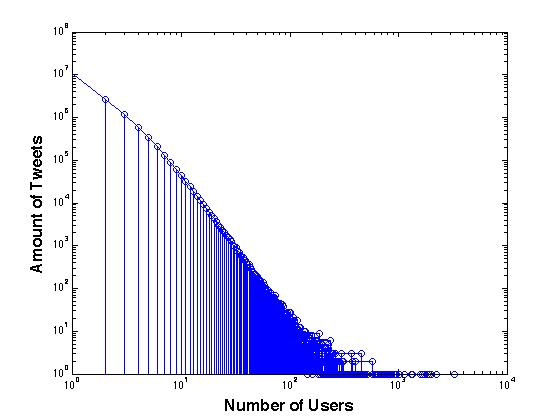
\includegraphics[width=\textwidth]{img/anal/loglog_users_tweets_1}
                \caption{LogLog: Number of Tweets per User}
                 \label{fig:u_log}
        \end{subfigure}%
        ~ %add desired spacing between images, e. g. ~, \quad, \qquad, \hfill etc.
          %(or a blank line to force the subfigure onto a new line)
        \begin{subfigure}[b]{0.5\textwidth}
                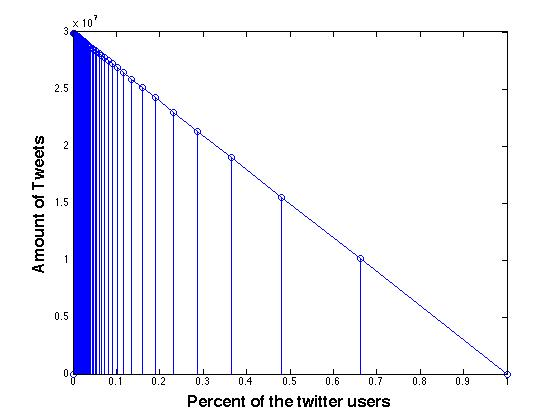
\includegraphics[width=\textwidth]{img/anal/no_power_1}
                \caption{Distribution: Number of Tweets per User}
                \label{fig:no_power}
        \end{subfigure}
        ~ %add desired spacing between images, e. g. ~, \quad, \qquad, \hfill etc.
          %(or a blank line to force the subfigure onto a new line)
      
        \caption{Volume of Tweets per Keyword and per Category}\label{fig:animals}
\end{figure}





\section {Food Term Distribution}

Our framework for the data acquisition successfully increased the total volume of food related tweets. From an initial 13.7 M tweets we raised the entire volume by 110\% to a total of 29.9 M food related tweets. The distribution of the volume per food term is displayed in Figure \ref{fig:world}. We illustrate in light grey the added volume alongside the initial size in dark grey. The most popular food terms on twitter are general terms such as \emph{food, dinner and lunch}. Within the 10 most popular terms we found that three beverages (coffee, beer, tea) were represented. The most popular traded commodity term on social media is chicken.  We further show the distribution of the categories in \ref{fig:cat}. By far the highest contribution has the category \emph{other food of interest} due to general food related keywords such as \emph{dinner} or \emph{food}. It builds the absolute majority with 51 \%. Meat related keywords have the second highest contribution with around 15 \% followed by 12\% sugar, 11\%  cereals, 10 \% dairy  and lastly 0.2 \% vegetable oils. We would like to note that the volume roughly follows the economic importance of the different categories with the only outlier being sugar \cite{fao2008}. We assume this is due to the highly popular products \emph{coca cola} and {chocolate} which caused alone 70 \% of the sugar related tweets. 



\begin{figure}[H]
        \centering
        \begin{subfigure}[b]{0.5\textwidth}
                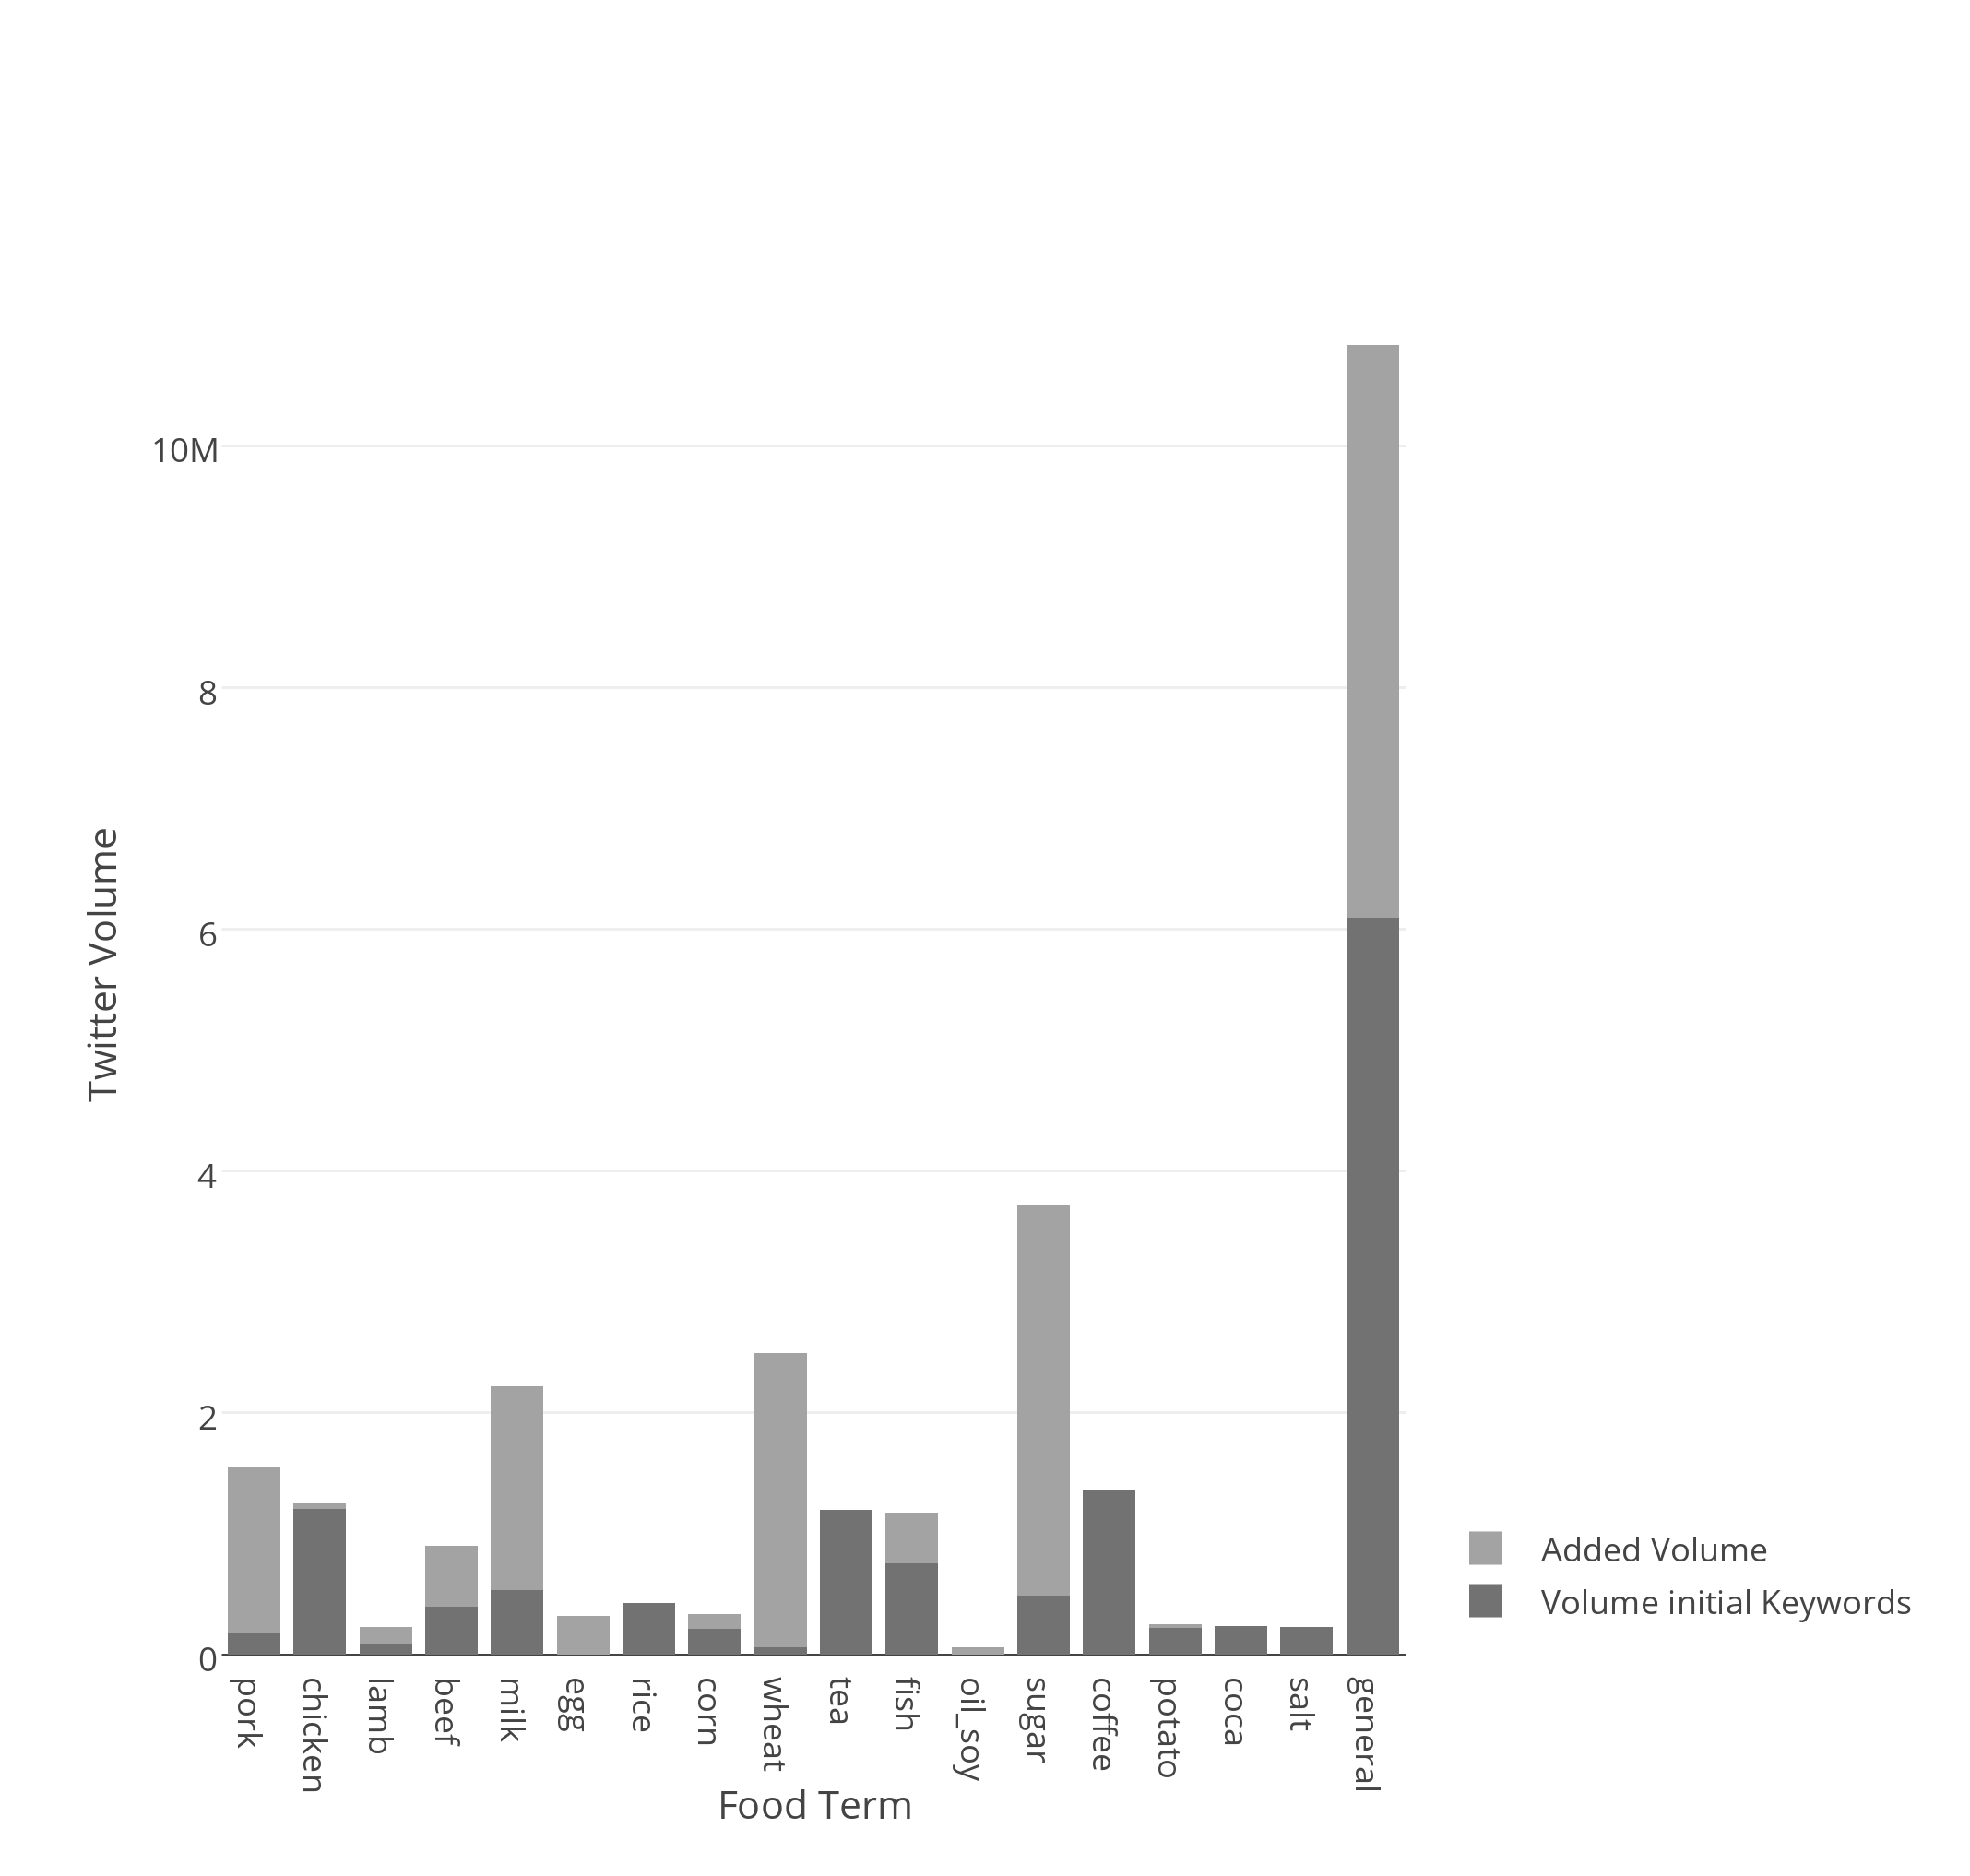
\includegraphics[width=\textwidth]{img/anal/exp_dist_1}
                \caption{Overall Distribution}
                \label{fig:world}
        \end{subfigure}%
        ~ %add desired spacing between images, e. g. ~, \quad, \qquad, \hfill etc.
          %(or a blank line to force the subfigure onto a new line)
        \begin{subfigure}[b]{0.5\textwidth}
                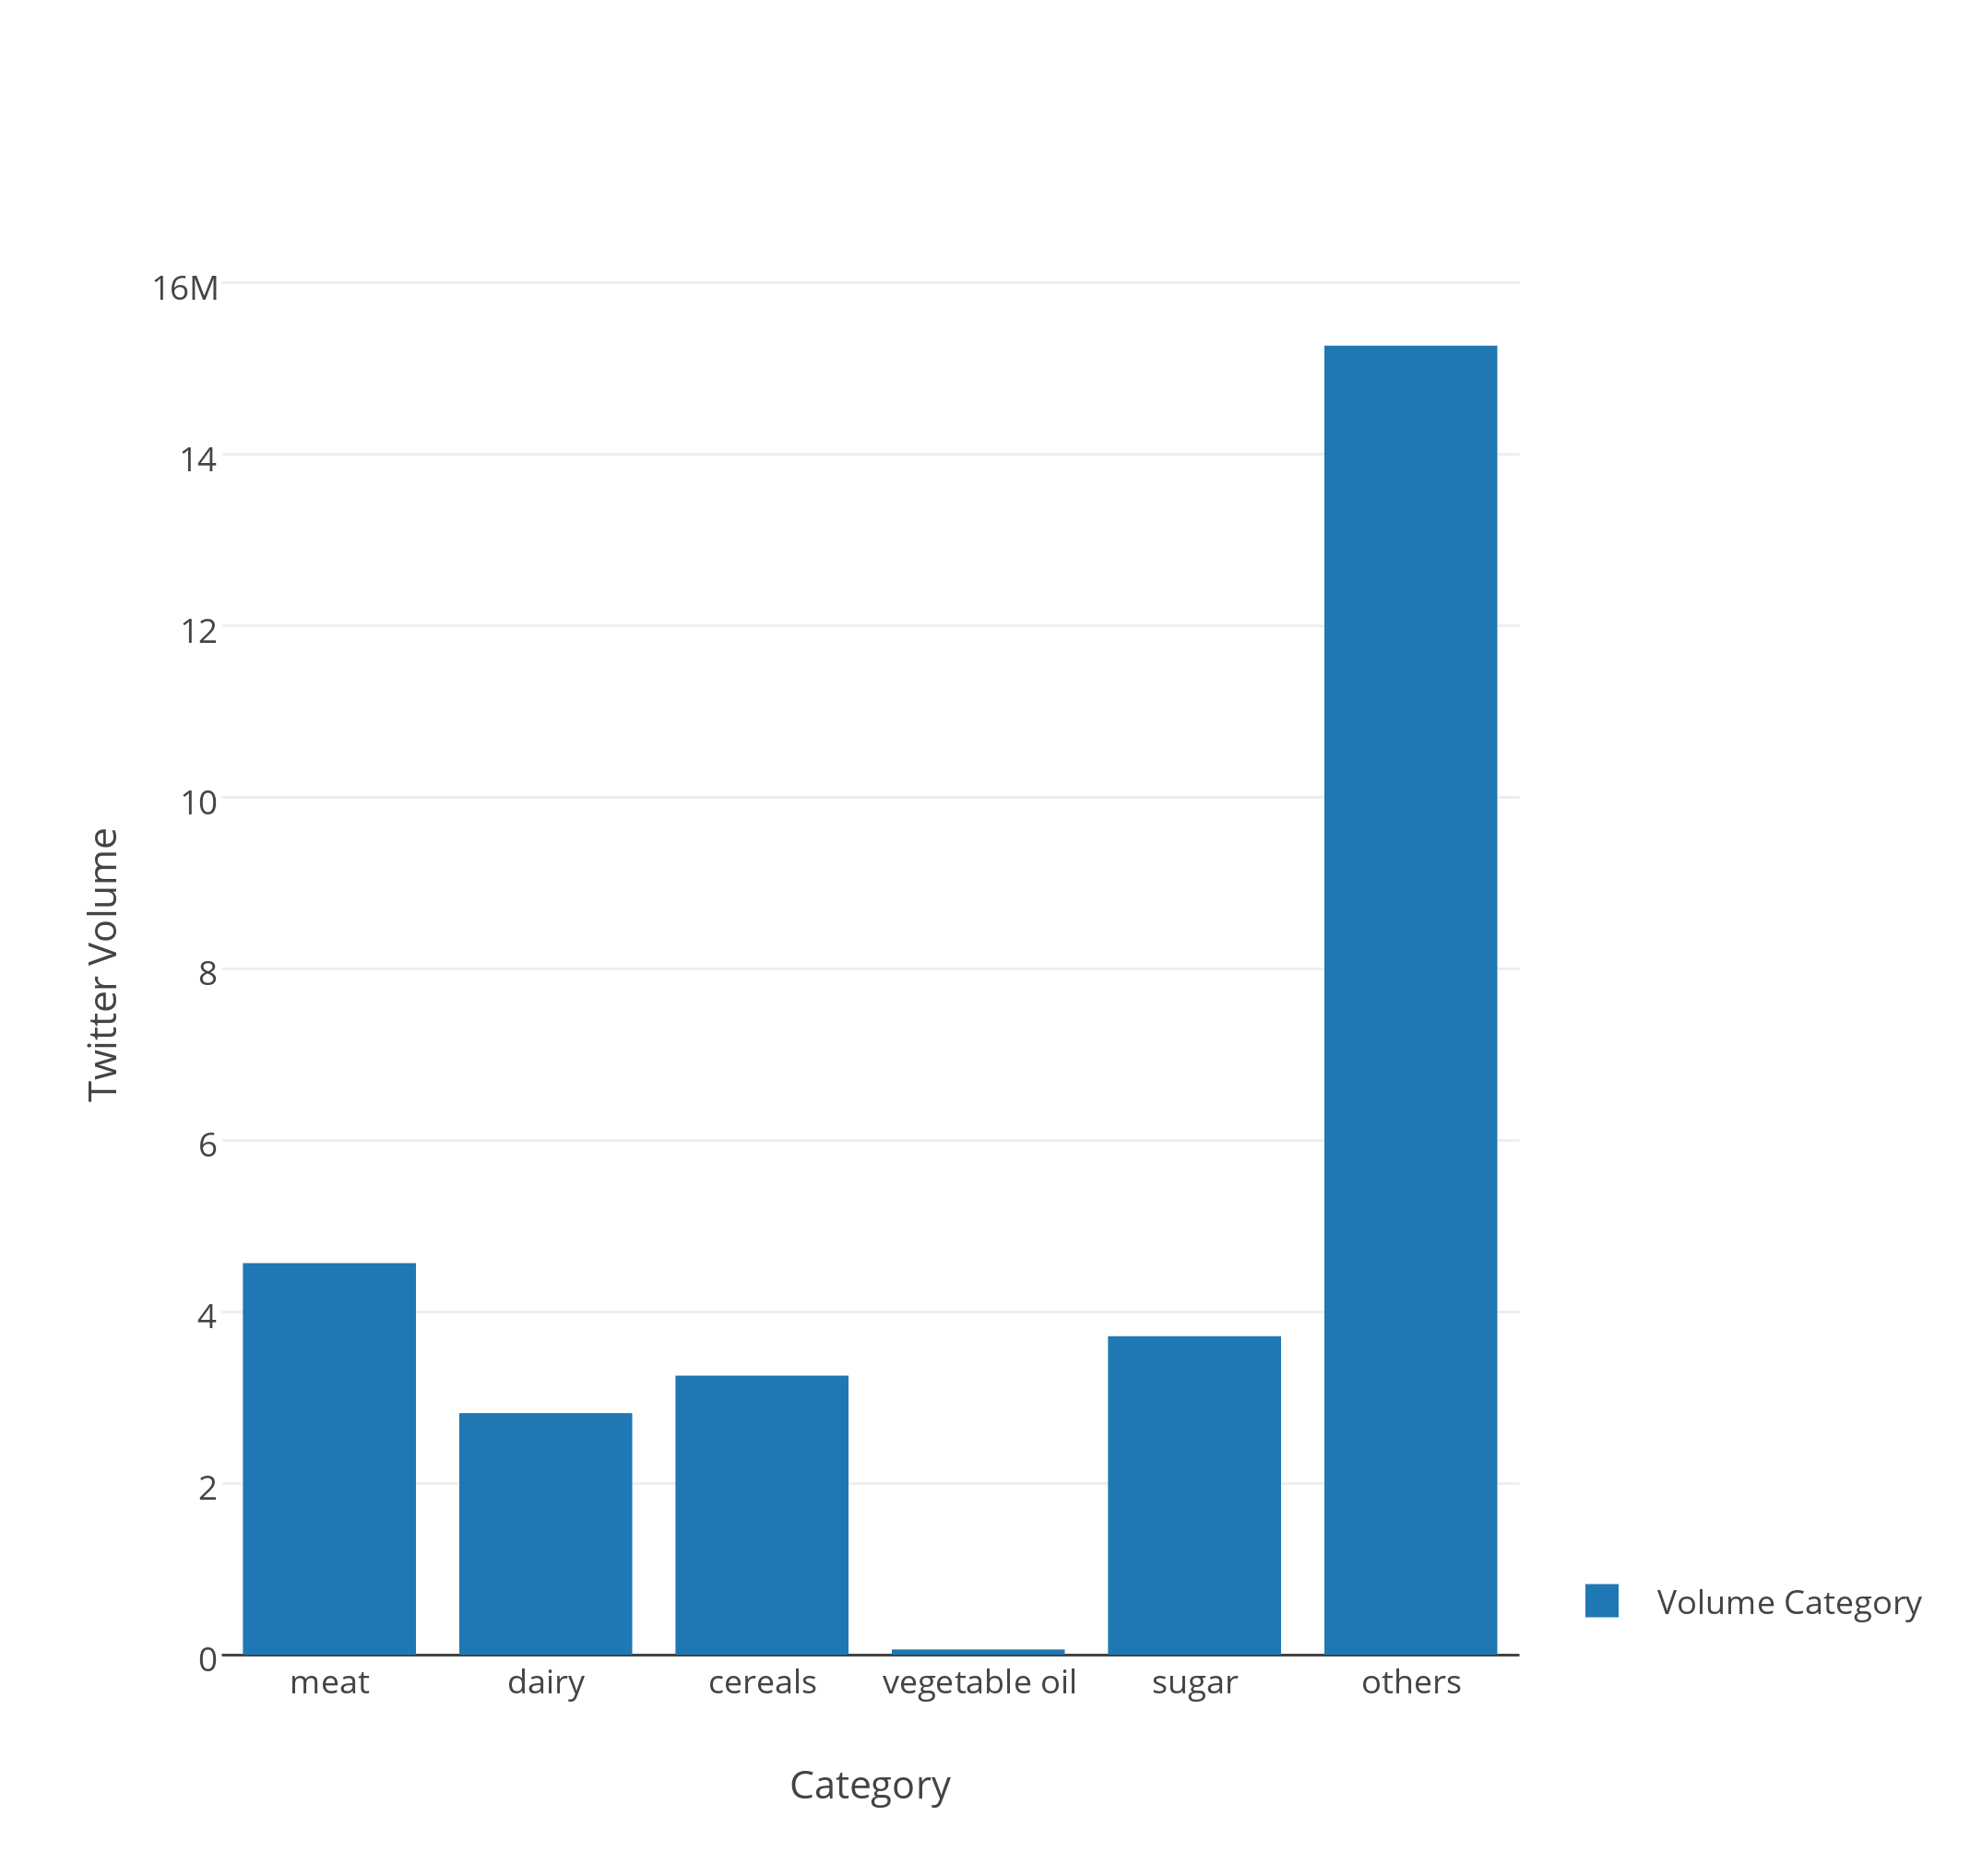
\includegraphics[width=\textwidth]{img/anal/exp_dist_cat_1}
                \caption{Category Distribution}
                \label{fig:cat}
        \end{subfigure}
        ~ %add desired spacing between images, e. g. ~, \quad, \qquad, \hfill etc.
          %(or a blank line to force the subfigure onto a new line)
      
        \caption{Volume of Tweets per Keyword and per Category}\label{fig:distribution}
\end{figure}


\section{Price Correlation}

%The weighted average of those five categories as illustrated in \cite{fao13}  defines the international food price index which is an overall measure of the current food condition. 

We observed a general popularity of food in our initial analysis and that certain food categories have a much stronger presence than others. There is however still a concern on whether the sampled data is useful to detect difference in price fluctuation and lastly can  be used as medium to determine food security. For the purpose of this correlation analysis we used the price quotations of the Food and Argriculture Organisation of the United Nations \footnote{http://www.fao.org/worldfoodsituation/foodpricesindex/en/} and commodity quotes from candle \footnote{https://www.quandl.com/}. FAO differentiates between a Category Food Price Index (CFPI) and a universal FPI. The CFPI is specific to a food category (e.g. meat, cereals) so different among all categories, where as the FPI is a general indicator and  the same for all categories. Unfortunately daily commodity quotes could only be obtained for meat, dairy and cereals. 

For each food category (e.g. \emph{meat, dairy} ) we correlated the tweet volumes of the subcategories( e.g. \emph{beef, chicken for meat}), products (e.g. \emph{bacon, salami}) and the price quotes for each category. These subcategories mirror the categorisation of the FAO \cite{fao2008}. Since the price quotes of the FAO are based on a monthly average, we aggregated the daily tweet volumes per food term over a month and calculated the daily average volume. We only included food terms that have an average of greater than 10 tweets per day. The internet archive did not contain tweets for certain months. We approximated those values by taking the average of the previous and the following month. 

\subsection{Results} 
\label{corr_results}

Between the meat subcategories there is a  positive linear relationship in the range of 0.7264 to 0.9361.This means if chicken increases in volume so does beef and pork. A $p$ value of 0.0001 suggest that we can reject the idea that the correlation is due to random sampling. No clear relationship exists between the tweet volume of the meat categories and the three price indices. Incase of a slight correlation most of the categories are negatively correlated to price quotes meaning that if the volume increases the price will most likely decrease. Only a few sub products showed a significant correlation with the price quotes. A positive relationship can be seen between the term goat and the commodity price with a correlation of 0.7369 and a p value of 0.0001. A possible explanation might be its popularity among developing countries. People consuming goat meat would be more sensitive towards price fluctuation making it potentially a valuable feature in measuring food prices. By correlating the price indices we see that there is a strong positive relationship between the FAO meat price index and the commodity quotes. This analysis supports \cite{abbott2009} theory that the commodity markets have a strong influence on the rising food prices and are a strong factor for quantifying Food Security. 



\begin{figure}[H]
        \centering
         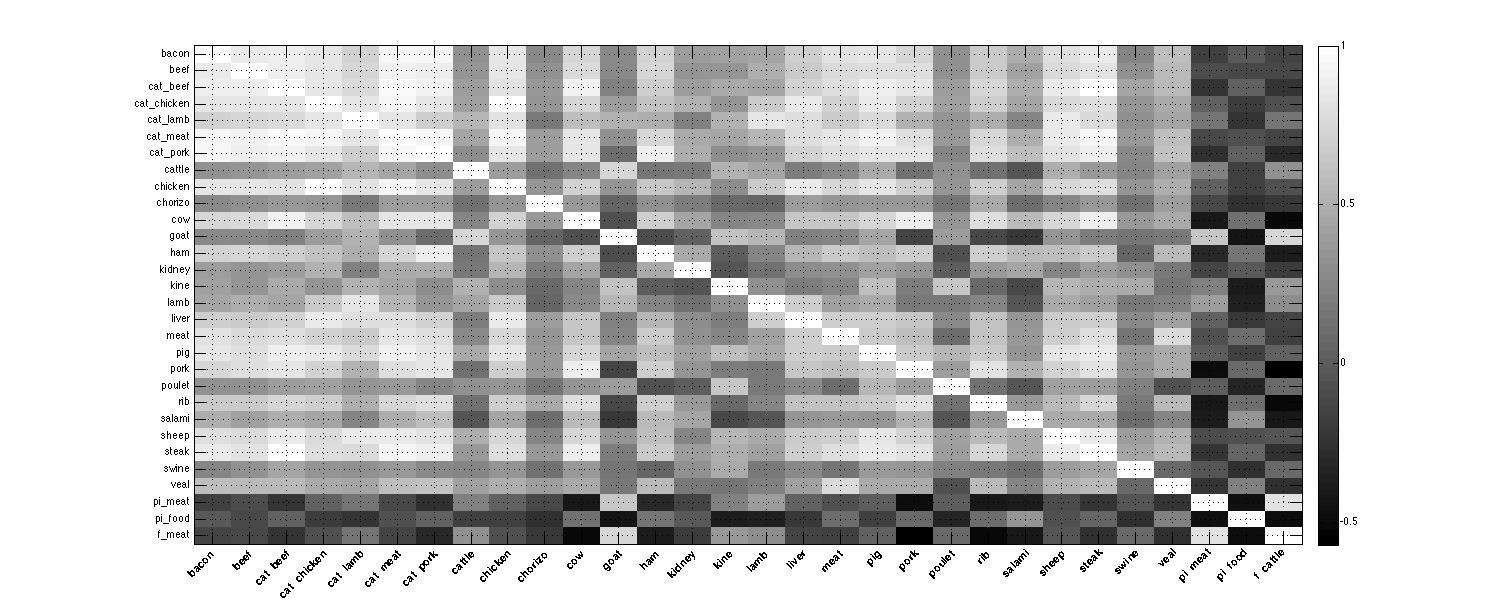
\includegraphics[width=1\textwidth ]{img/anal/meat_black}
              
        \caption{Heatplot Meat: Volume of Tweets per Keyword and per Category}
        \label{fig:distribution}
\end{figure}



For cereals similar to meat we likewise see a high correlation in volume of around 0.82 between the different cereal categories. The products \emph{beer, barley, bread, atta and pasta} show a strong positive relationship to the cereal categories. Unlike meat, the cereal category price index and the commodity price show a strong positive relationship with the universal FPI. This is somewhat surprising as meat prices have a stronger influence on the universal FPI then cereals do \cite{fao2008}. Furthermore the product pasta has a strong linear relationship with the commodity price of 0.7212.
\begin{figure}[H]
        \centering
         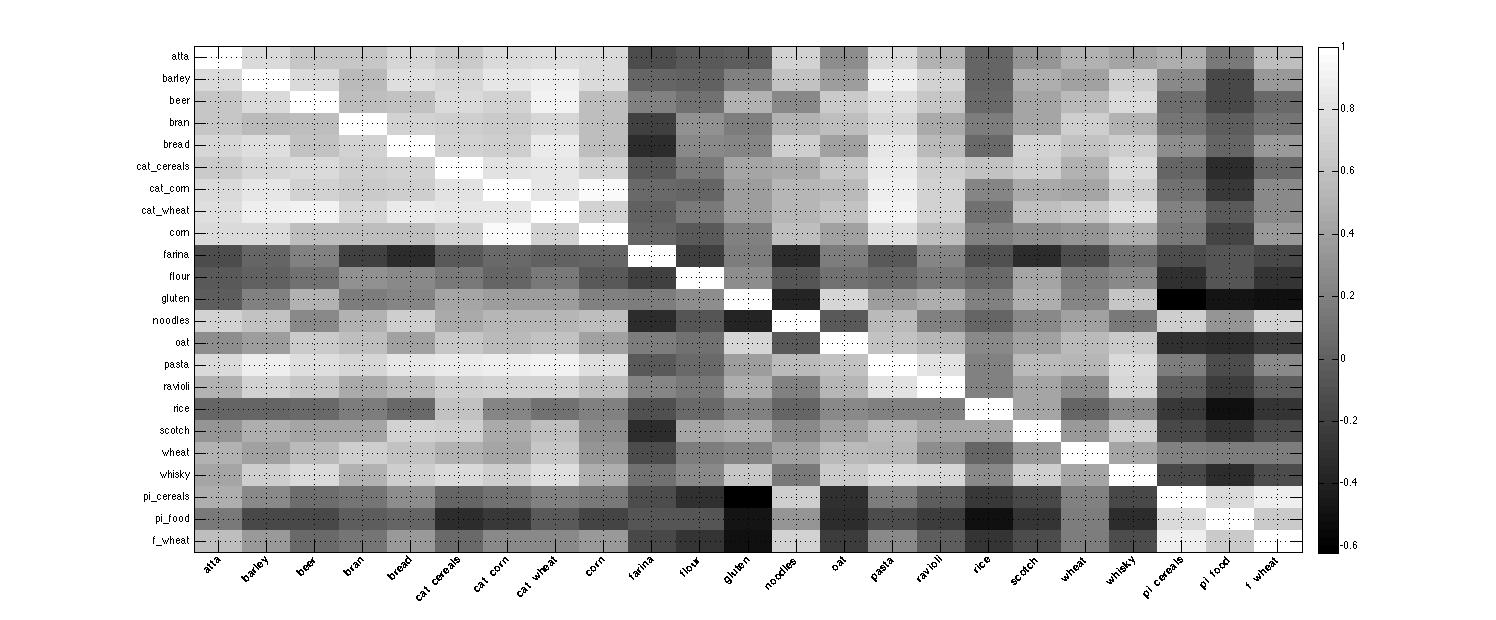
\includegraphics[width=1\textwidth ]{img/anal/black_cereals}
              
        \caption{Heatplot Cereals: Volume of Tweets per Keyword and per Category}
        \label{fig:distribution}
\end{figure}
 

The heat plots of dairy, sugar and oil show yet again no clear linear relationship between the twitter volume and the food price indices. More so than in other food categories the subcategories of dairy can be clearly distinguished through its strong correlation with the different products (i.e. mozzarella has a strong relationship with the category cheese and only a weak correlation with milk products). The heat plot for dairy, sugar and oil have been added to the appendix \ref{pCorr}.



\subsection{Discussion} 

Our analysis did not show a significant correlation between the raw attention on food and the price quotes.
Nonetheless the insights gained from this analysis will help us improve our features. For example the category meat shows a number of products that have a strong negative correlations. By only including such terms we are hoping to strengthen the relationship between the meat category and the price quotes.

 Although we can not provide any scientific evidence there might be a nonlinear relationship between social media and the commodity market. We hence will experiment with a non-linear model to predict price quotes in Chapter \ref{model}. According to \cite{de08} such models are better suited to utilise social media for predictions. 

A smilier correlation analysis has been made by the UN \cite{ungp2013}. They however used contextual sensitive tweets i.e. instead of only using tweets containing food they performed an n-match on different criteria. The tweet had to contain a food item, the word price and a quantification such as high or low. Overall a Pearson correlation of around 0.42 was detected with a significance of 0.04. By exploiting our predictor lexicon to filter tweets that contain keywords such as supply and price we were able to improve the linear relationship and found similar results as in \cite{ungp2013}. Although the UN concluded a linear relationship they simply provided assumptions about what might have caused the volatility of price conversations. We hence explore the conversation drivers in the next section. 
 

 
\begin{table}[h]   
 \begin{tabular}{  c  | c  | c | c }
			
   & \textbf{Category Price Index}  & \textbf{Food Price Index} & \textbf{Commodity Price Index} \\
  \hline 
  &&& \\
  Meat & -0.0112   & -0.0653 & - 0.1489  \\
  
  Dairy & -0.2166   & 0.1314 & -0.0676\\

  Cereals & 0.0357  & -0.3360 & 0.0594 \\

  Oil & -0.2484  &  -0.2382 & -   \\

  Sugar & -0.2000 & -0.1019 &  - \\

\hline 

\multicolumn{3}{c}{\null}\\

\multicolumn{3}{c}{\textbf{Significance:} p $<$ .0005 ***, p $<$ 0.005 **, p $<$ 0.05 *}\\
\hline  

\end{tabular}
\caption{Price Correlation}
\label{tab:abc}


\end{table}


 \section{Conversation Drivers}
 \label{conversation}


Following our correlation analysis we proceed with a detailed investigation of twitter conversations relevant to food security to uncover events that trigger conversations. We found that our contextual sensitive tweets (i.e. such tweet that contain a food term and a predictor term such as price) have a stronger Pearson correlation than the raw volume. Encouraged by this observation we want to investigate further to which extent the tweet content is related to food security. More specifically we want to know if the conversations can be related to market fundamentals that cause soaring food prices. Following the two recent food crises in 2007 and 2010 a lot of research has been centered around defining causes of volatile food prices.  In \cite{Tadesse2014} they define a taxonomy for drivers of  international food price spikes and differentiate among three different causes namely exogenous shocks, conditional causes and internal causes. Examples of exogenous shocks are extreme weather events, oil price shocks, economic and demand/supply growth, and lastly economic shocks. Conditional causes can originate through political conflict or market conditions. Internal causes on the other hand are speculative activities(driven by price expectations) and declines in world food stocks. This taxonomy will serve us as a baseline in annotating our events. 



\subsection{A Visual Analysis of the Social Attention}

We commence our investigation of the conversation drivers by a visual and manual investigation of the most prominent events. To gain an overview about the social attention of our food topics we plotted the relative distribution of food supply, price poverty and needs in Figure \ref{fig:topic_dist}. By far the highest attention is attributed to food needs with around 70 \% , poverty and supply receive a similar attention distribution with price taking the smallest interest among twitter users. 

To visually categorise the activity, Lehman et al. \cite{Lehmann2012} defined three categories of temporal behaviours. Continuous activity, periodic activity or activity concentrated around an isolated peak. Continues activities are topics that are of daily interest such as weather. On the other hand periodic actives reoccur with a fixed pattern such as the release of a popular Tv show. The latter is event driven and usually occurs once during a very short period such as a national holiday. 

For price and supply we observe a similar temporal pattern. Both show a continuous activity with one extremely prominent isolated peak. The activity is concentrated symmetrically around those two events , showing abnormal activities for around 9 days before and after. 

 We manually investigated the two isolated peaks to see if we can attribute them to any discussions relevant to food price or food supply. Surprisingly, the content in the price discussion corresponds to a popular Korean pop band \emph{T-ara }. \emph{T-ara } released a music video on the 10th of September which caused the first anomaly, reaching a global maximum on the 16th when they announced to collaborate with a famous European DJ  \footnote{http://www.kpopstarz.com/articles/112632/20140916/t-ara-sugar-free.htm}. Similarly, in our supply conversation the peak was not caused by supply indicators but was driven by conversations centered around health \& life style topics. 

The topics needs and poverty do not exhibit any extreme outliers and similar to price and supply can be categorised according to Lehman et al's. framework as of continuoes interest. 




\begin{figure}[H]
        \centering
         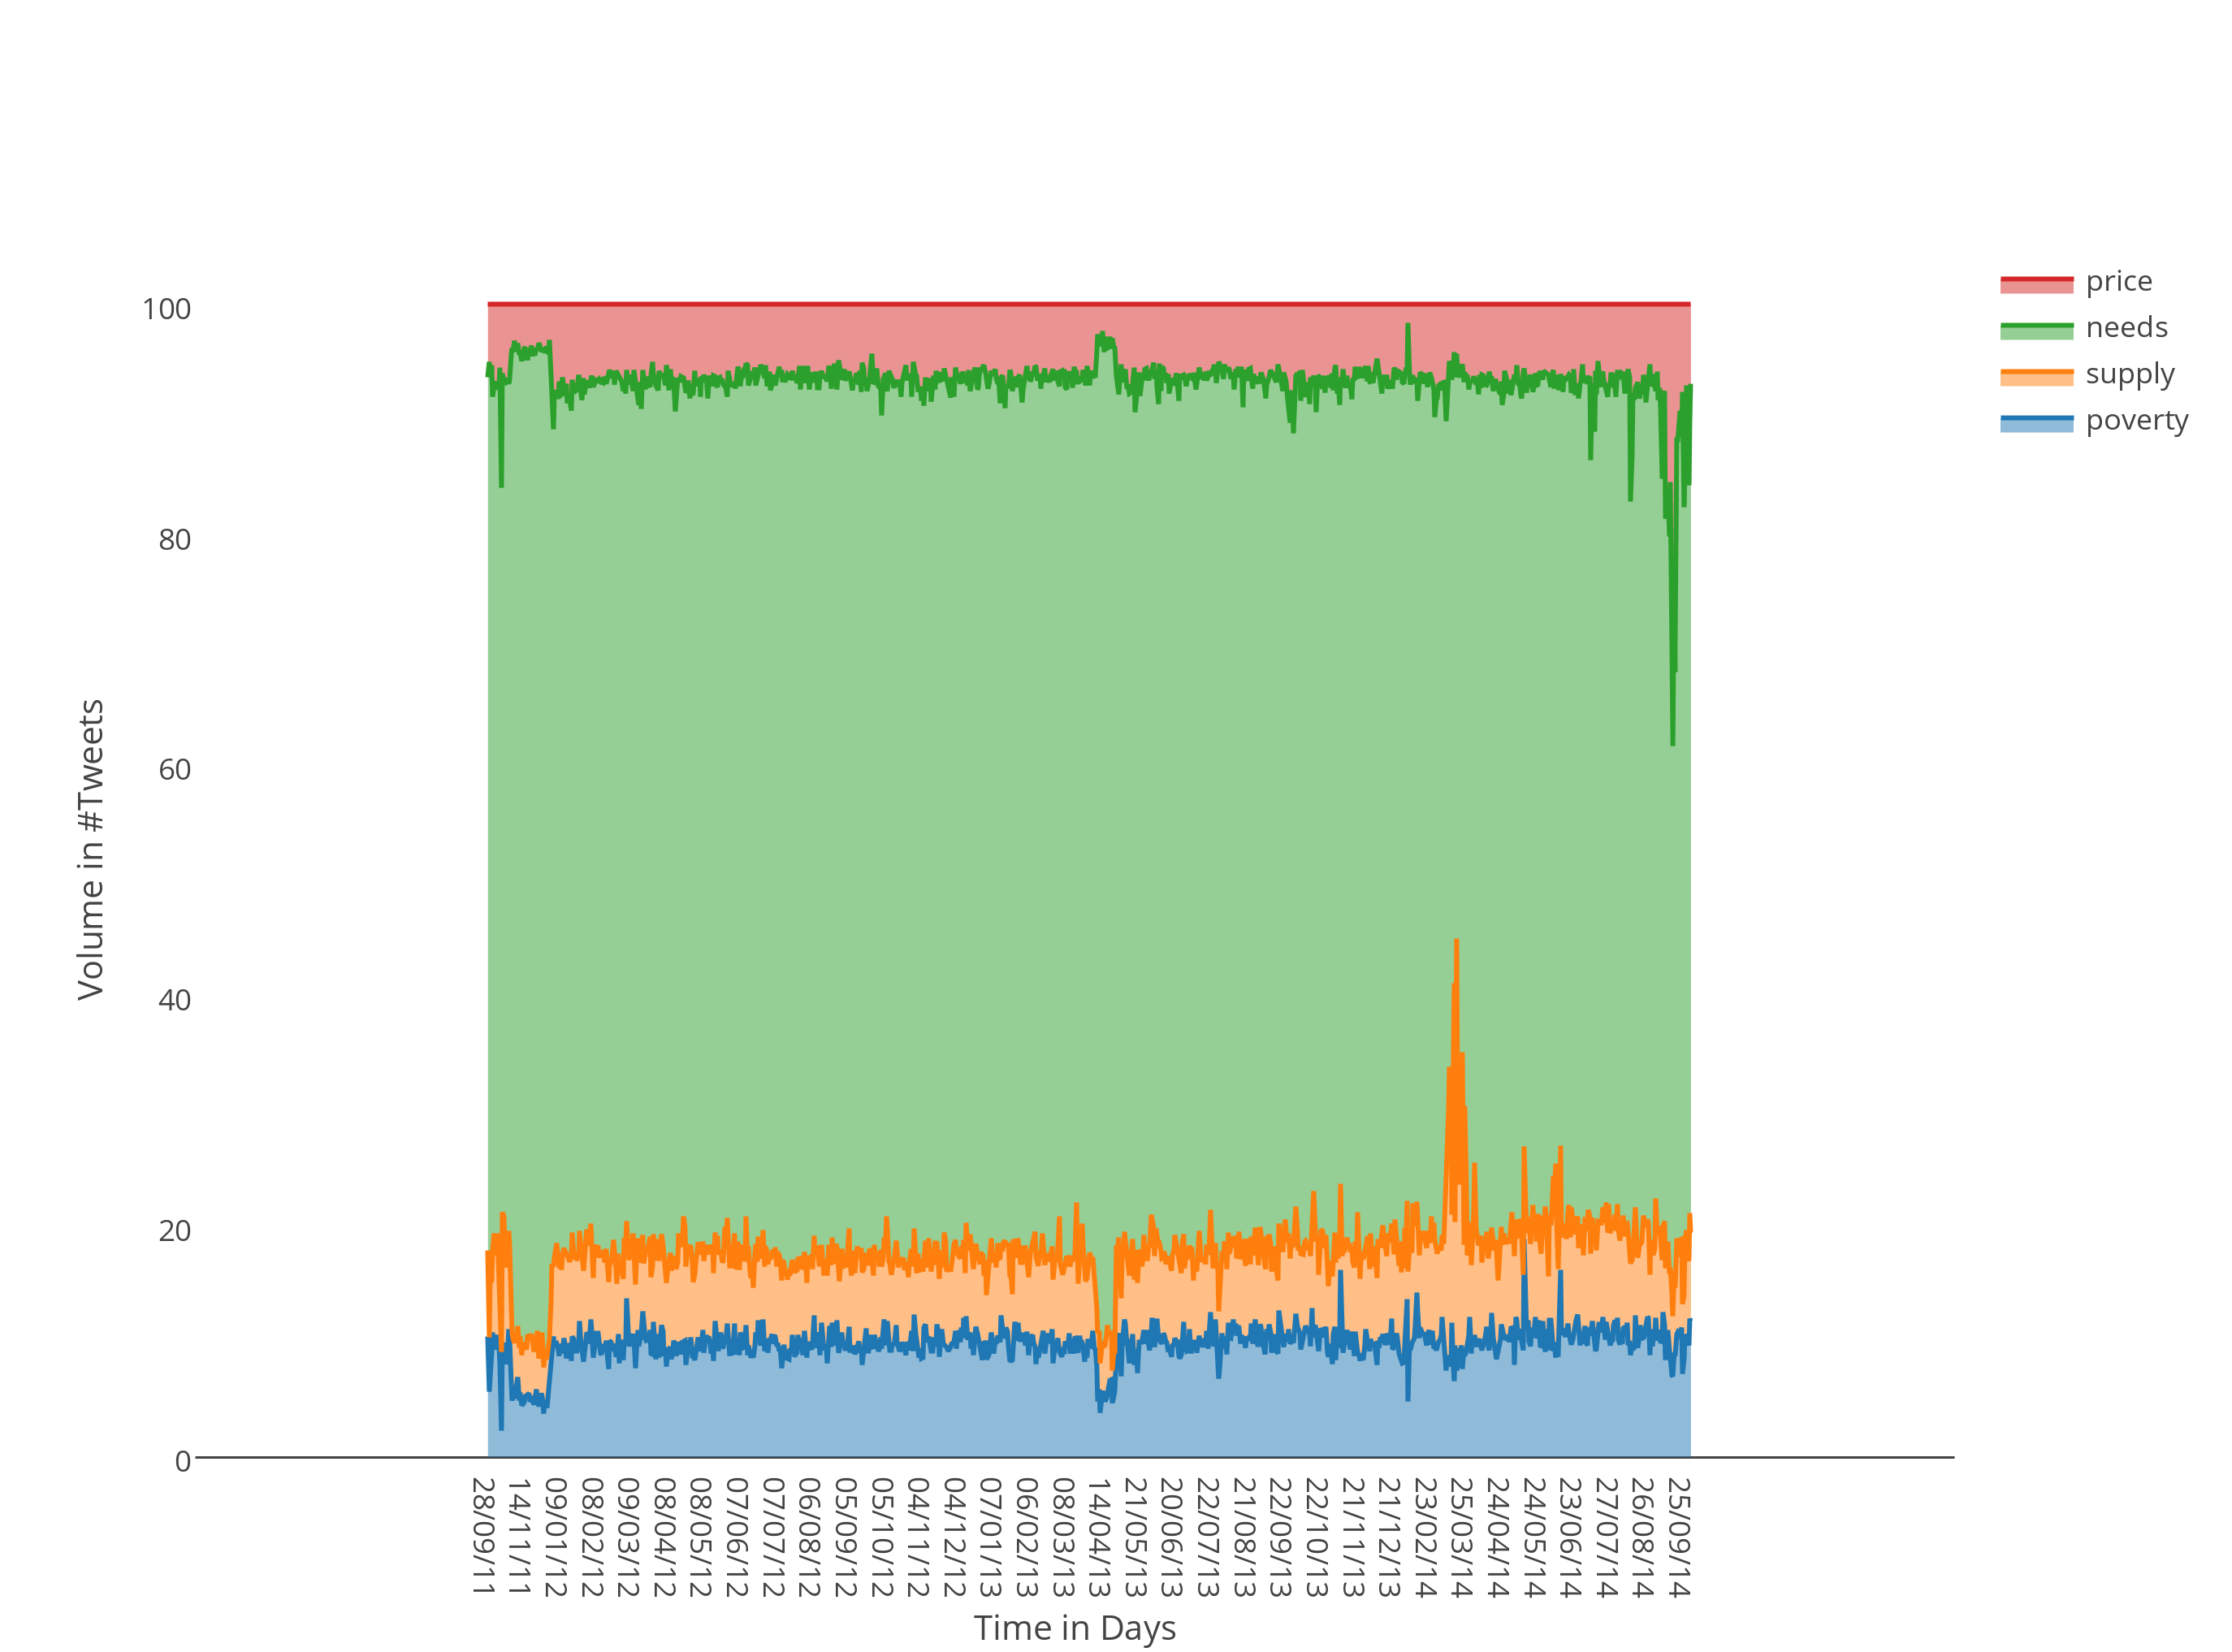
\includegraphics[width=1\textwidth ]{img/anal/topic_dist}
              
        \caption{Topic Distribution - Food Security}
        \label{fig:topic_dist}
\end{figure}




\subsection{Methodology} 

As described in the previous section the prominent peaks could not be attributed to any discussion around indicators that are relevant to Food Security. In this subsection we investigate in detail what topics cause the attention peaks and whether they can be attributed to market fundamentals or topics concerning Food Security. For this analysis we consider discussion around food supply, price, needs and poverty. 
We investigate the four food categories temporal behaviour on a granularity of one day. This scale was chosen in order to be in accordance with the temporal quotations of the commodity market. 
To detect anomalies in our food topics we applied a similar approach as in \cite{olt15} \cite{Lehmann2012}. We used a fixed window size of $2m + 1$  where $m = 15$ giving us a month long window. Within the window we identified the median and calculated the mean of the twitter volume. From those values we calculated the Median absolute deviation (MAD) as in Equation \ref{eq:mad}: 

\begin{equation} \label{eq:mad}
\overline{ MAD } = median_i (|X_i - median_j(X_j)|)\end{equation}


$X_j$ is the set of data points within the fixed window and $X_i \in X_j$

A peak is declared if $v_i$ deviates more than 2 MAD from the mean. For this analysis we only consider positive peaks and ignore anomalies in form of a steep descent. 

The discussion centered around food price showed 82 events. Tweet activities for food supply resulted in 91 peaks. 80 peaks were detected for food needs and lastly 99 for food poverty. 
 

To identify what topics spike the attention we used a similar approach as in \cite{olt15}. We computed the top 50 unigrams and top 10 bigrams of all tweets occurring during a peak. We then manually investigate the tweets that contain the most frequent n-grams. Some peaks could be attributed to multiple events. If two could be identified, both of them were used to label the peak. Else, if most likely more than two events caused the peak we marked it as ambiguous.  

\subsection{Event Annotation}

We annotate each peak according to the definitions given bellow. Our classification mostly mimics the main dimensions of Food Security but also includes categories from the taxonomy of Tadesse et al\cite{Tadesse2014}. There is a strong overlap between the two taxonomies where the later naturally focuses more on Economic Access and the former has a stronger orientation towards Food Utilisation. This categorisation is not extensive i.e. there are a range of further categories we could consider. However given the sparsity of relevant events this classification gives a good overview of the discussed topics. 

Some events show causal relationships i.e. a breach in the food supply can be a cause for riots and political unrests. In such cases we annotated both. 


\begin{description}
  \item[Food Supply ] \hfill \\
 Events entered around the food supply chain are considered including indicators of food waste. We define Food Loss and Food waste according to Parfitt et al. 's \cite{Julian10} definition. Food Waste refers to Food Loss that occurs at the retailers and consumers side where as the term Food Loss refers to the decrease in food volume that leads to edible food for consumption.
  \item[Economic Access] \hfill \\
  We define Economic Access according to FAO's \cite{fao2008} definition. Price, expenditure or market indicators fall into this domain.   
  \item[Government] \hfill \\
  The classification Government takes topics such as legislation and policy changes into account. An example is restrictive trade policies such as export or import restrictions  \cite{Tadesse2014}. 
    \item[Stability] \hfill \\
 Poverty,  political unrest and topics concerning extreme weather \cite{fao2008} fall into this classification. Factors that cause insecurity such as riots or severe draughts are considered. 
    \item[Unrelated] \hfill \\
   Viral jokes,  advertisements, health \& lifestyle are example topics that we consider unrelated. 



\end{description}








Our findings showed that for price only 7 (8.5 \%) out of 82 fell into the above given categories, for  supply 4 (4.3 \%) out of 91 for poverty 13 ( 13 \%) out of 99 and finally for needs no relevant topics were found. 


\subsection{Results}
\label{an_result}

The distribution of the annotations is visualised in Figure \ref{fig:annotation_dist}. Surprisingly the conversations mostly peaked outside their domain, i.e. the price conversation was more intrinsic for supply indicators then for economic access indicators. We now give examples to each annotation topic of events that we classified as Food Security relevant to illustrate what kind of discussion caused a peak . 



\begin{description}
  \item[Food Supply ] \hfill \\
 Topics that caught the social media audience were especially safety threats to the food supply. In April 2012 a newly discovered case of cow disease threatened the safety of America's beef supply and heavy import restrictions were imposed from major beef importers such as South Korea \footnote{http://www.theguardian.com/science/2012/apr/25/mad-cow-disease-us-mutation}.
  \item[Economic Access] \hfill \\
  In 2014 sharp rising food prices caused a lot of discussion on twitter. Wholesale prices were suffering due to a severe drought in the previous year, which thinned the cattle herds and increased consumer prices \footnote{http://www.cnbc.com/id/101588110}. As a consequence there was also a sharp increase in discussion around food banks. The UK observed a 51 \% increase in food bank users \footnote{http://www.bbc.com/news/business-27032642}. 
  \item[Government] \hfill \\
  Most discussions around legislation changes were focused on Food Bank reforms. A high amount of attention can be attributed to the UK rejecting the European Union food bank funding. The population heavily criticised the British government to deny EU fund to be spent on the poor \footnote{http://www.theguardian.com/society/2013/dec/17/government-under-fire-eu-funding-food-banks}
    \item[Stability] \hfill \\
  Discussions around stability were usually headlined by extreme poverty causing riots. A food program that provided free lunch to underprivileged school kids used poisoned crops in their dishes. 20 children died as a consequence causing riots and closed shops all over the city. \footnote{http://www.usatoday.com/story/news/world/2013/07/17/india-children-deaths/2523727/}
   \item[Unrelated] \hfill \\
   Unrelated topics cover a vast amount of domains. Most often peaks are caused by viral tweets posted by online celebrities that contain a food term. Public holidays, such as Easter, Thanks Giving are also frequently captured. Furthermore public figures such as Ray Rice, a famous football player, caused a lot of hype in the social media community \footnote{http://www.nytimes.com/2014/09/09/sports/football/ray-rice-video-shows-punch-and-raises-new-questions-for-nfl.html}. Often it was very hard to extract the conversation drivers in the unrelated topics. There is a considerable amount of noise in our conversations centered around Food Security, making it very challenging to extrapolate meaning from an event. This might be attributed to the general popularity of food we identified in previous chapters. 

\end{description}




\begin{figure}[H]
        \centering
         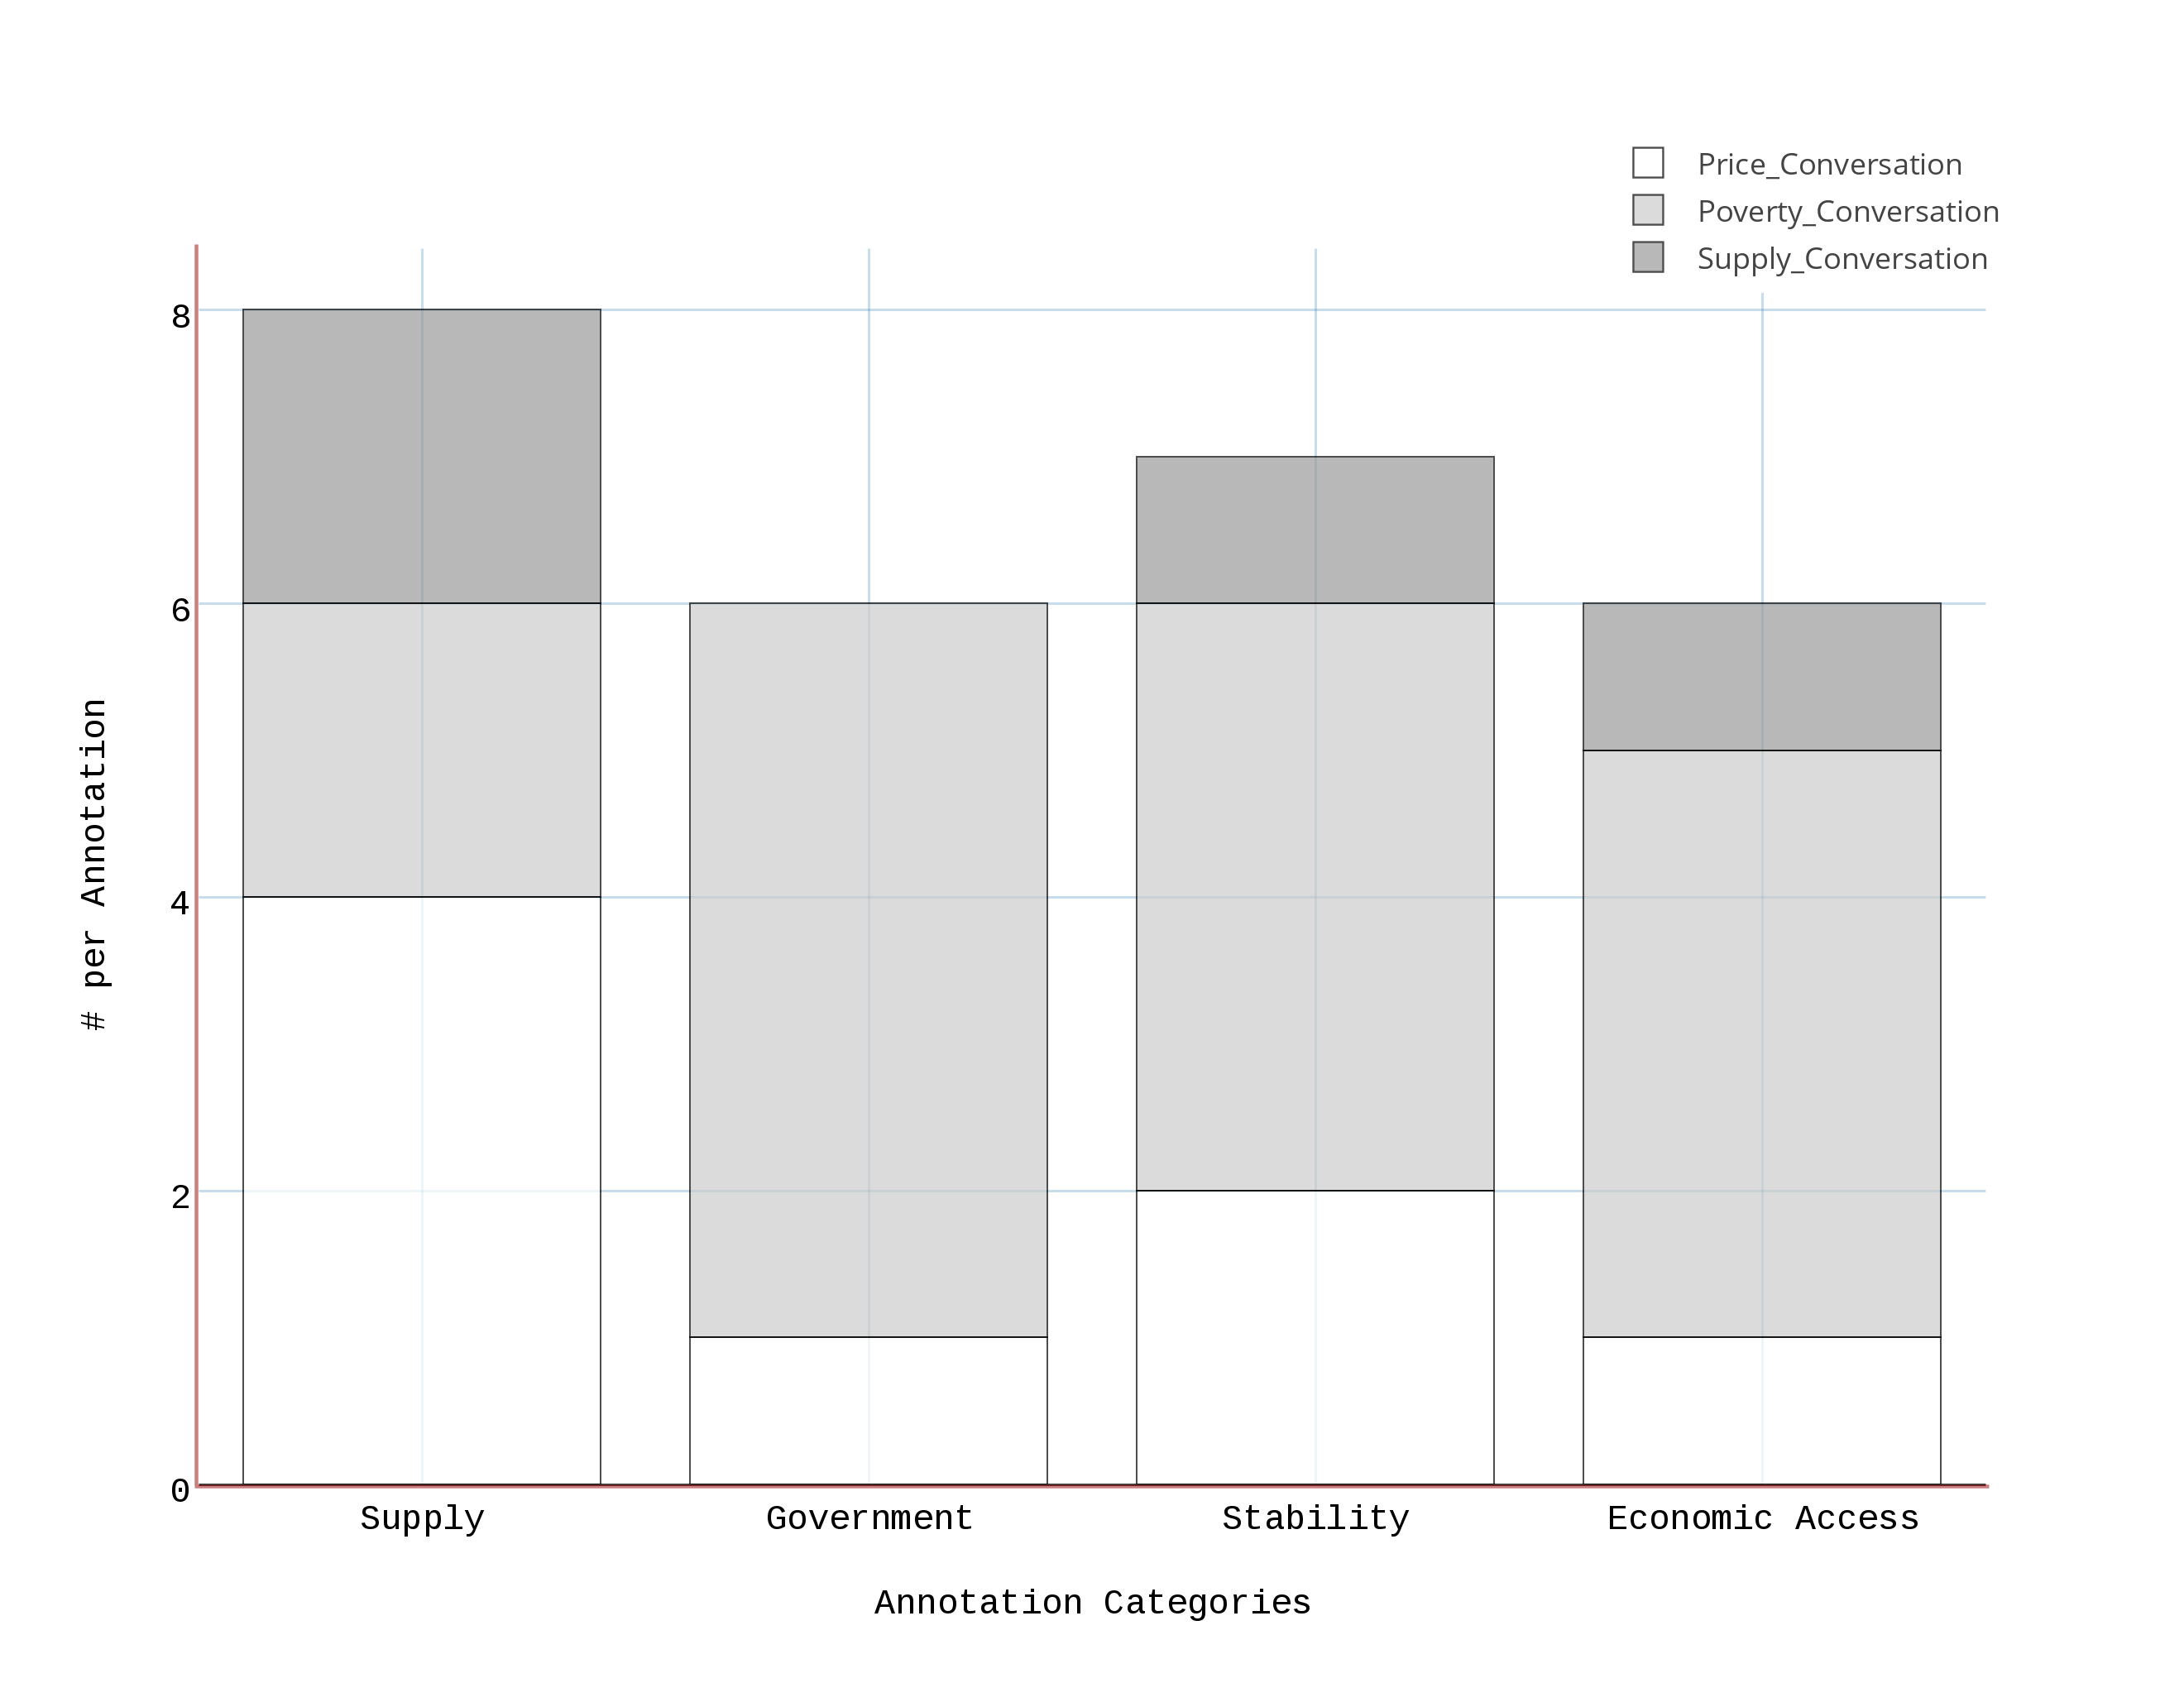
\includegraphics[width=0.7\textwidth ]{img/anal/annotation_dist}
              
        \caption{Annotation Distribution - Relevant to Food Security}
        \label{fig:annotation_dist}
\end{figure}


\subsection{Discussion}

Extracting information from noisy and unstructured text has shown to be a very difficult task. Despite our various filtering attempts there is still a substantial amount of noise in our food security discussions. As most of the volatility was attributed to unrelated topics we will have to rethink the way we use the twitter data as a feature in our model. Unrelated does not necessarily mean irrelevant. Even twitter discussion outside our food security objectives can provide valuable information. Most commonly this is achieved by analysing the attitude of a tweet's author. We will hence explore the entropy of sentiment in explaining volatile food prices. 




\chapter {Model Building}
\label{model}

Intro goes here ......

\section{A fuzzy approach for Time Series Modelling}

Compared to other approaches, Fuzzy logic has seen only a few applications in forecasting despite its promising results. We hence want to motivate the use of this technique in further detail. 

Fuzzy logic was initially proposed to provide a framework for imprecise reasoning. Zadeh \cite{Zadeh65} introduced the concept to describe real world phenomenas that do not have precise description of a membership class. Another branch of mathematics that deals with uncertainty is the field of probability. However, there is a distinct difference between the two. Probability theory is based on Bivalent logic, which means every proposition is either true or false. Only certainty is a matter of degree, which brings us to an important distinction. In Fuzzy logic everything is a matter of degree, which is ultimately how we perceive the real world. This form of reasoning allowed the development and analysis of  systems by expressing the qualitative aspects of human reasoning without using any complex mathematical models \cite{Jang91}.  
In some areas such as time series prediction techniques such as ARMA and AR, have shown clear limitations \cite{box90}. Nonlinear approaches, such as ANFIS, have proven to be more successful \cite{chap04}. Prediction accuracy is however not the only concern in forecasting models. Understanding the behaviour and gaining insight into the underlying dynamics is equally important \cite{neil93}. This make ANIFS especially appealing. Not only does it poses strong predictive capability but as a consequence of its rule based design it allows for interpretability of the predictions. This is particularly important as the results might help us better understand the determinants of food security risks in social media. 

\section{Fuzzy Logic}


In this section we present the terminologies and concepts around Fuzzy logic, focusing on the basics of Fuzzy variables, and Fuzzy sets, as well as how a Neural network is derived with a Fuzzy interference system (FIS). 

\subsection {Fuzzy Variables and Fuzzy Sets }

Zadeh \cite{Zadeh65}  defined Fuzzy variables as attributes that distinguish between elements of some universe of discourse ( this is achieved by mapping input variables to a unit interval). He uses the colour of an object as an example. Each colour is defined by its wavelength, which is a precise numerical definition. In natural language we tend to classify colours not by its numerical value, but by colour objects (e.g. red, blue, green), which fall into the scope of a specific wavelength or how it is commonly referred to in Fuzzy logic,  a Fuzzy set. Red or blue describe the object's colour, but it is by no means a precise definition. By applying a membership function we can precisely define the colour in a range between zero and one. The most common membership functions are Gauss function, Trapezium function and the Triangle function. We choose to use a Gaussian membership function defined by Equation \ref{eq:gaus},  as they are differentiable and desirable for optimisation purposes \cite{wu12}. We will refer to $a_i, b_i, c_i$ as the parameter set.  

\begin{equation} \label{eq:gaus}
\mu_A(x) =  \frac{1}{ 1 + |\frac{x- c_i }{a_i}|^{2b_i}  }\end{equation}


With regard to our Fuzzy logic system we will distinguish between input variable and output variable. The output variable depends on the input value's corresponding membership function and a decision matrix, where the later will be explained in the following sections. 

 To illustrate the two concepts Fuzzy logic and Fuzzy sets at a concrete example, consider Figure \ref{fuzz_example}. The scope of each colour object (red, green, blue) is precisely defined by the three triangular functions. The colour object green is precisely green at the point $x_2$ and partly green between $x_1$ and $x_2$ and likewise $x_2$ and $x_3$. 
 
For this exercise we classify the colour object of a tangerine which is orange.  We define orange to be a little red (where little is a value between 0 and 1) corresponding to $y_r$ and very green corresponding to $y_g$.  The membership function would map those two input variables to $x_i$, where $x_i$ is our output value and a precise numerical definition of the colour object orange. This toy example generalises to any other object. The object price would be modelled with the triangular functions high, medium low sentiment on the other hand would use positive, negative or neutral instead. 






\begin{figure}[H]
        \centering
         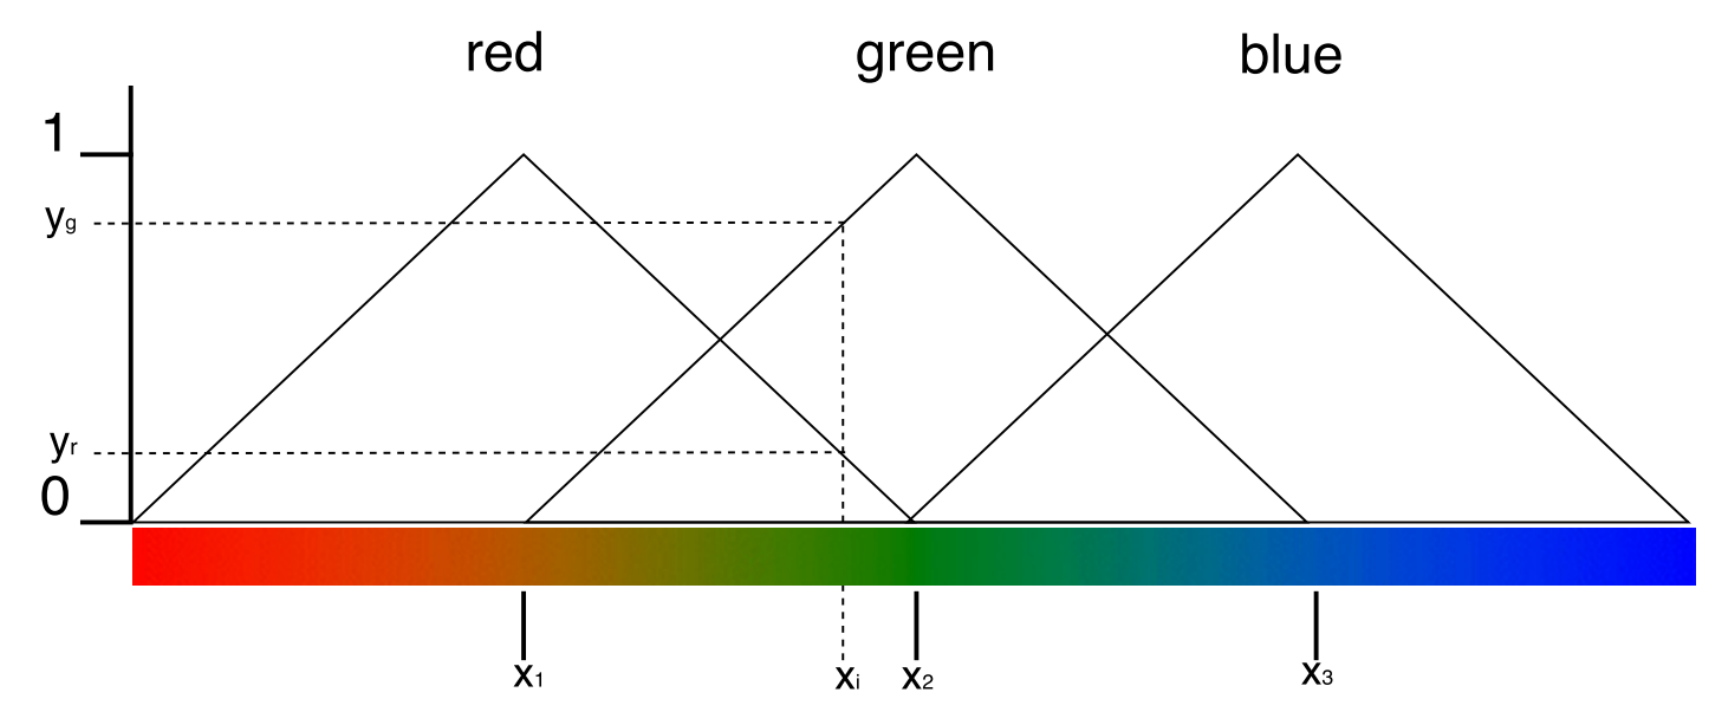
\includegraphics[width=0.7\textwidth ]{img/model/fuzz_example}
              
        \caption{Fuzzy Variables and Fuzzy Sets - A Colour Object Example}
        \label{fig:fuzz_example}
\end{figure}



\subsection{Fuzzy Interference System}

We first describe the components of the Fuzzy interference system (FIS) and then give intuition on how the system can be modelled as a Generalised Neural Network (GNN). 

FIS evaluates a decision matrix composed of rules in the following semantic: \\

\centerline {$ \textbf{IF} <  A  > \textbf{AND} <  B  > \textbf{THEN} < Conclusion > $}

The rule base grows exponentially with the number of variables. Hence, we have to carefully consider the input variables in order to minimize the complexity and to make the inference reliable. A multivariable system uses two different kinds of connectives to combine the fuzzified values. The union is defined in Equation \ref{eq:union} as the \emph{multiplication} of the membership function of set A $\mu_A(x)$ and B $\mu_B(x).$ The result is a weight $w_i$


 \begin{equation} \label{eq:union}
 w_i =  \mu_{A\cup B(x,y)} =   \mu_A (x) \times \mu_B(y)
 \end{equation}

The intersection is defined in Equation \ref{eq:probor} as the \emph{probabilistic OR} of the membership function of set A $\mu_A(x)$ and B $\mu_B(x).$ 
\begin{equation} \label{eq:probor}
 w_i =  \mu_{A\cap B(x,y)} =   \mu_A (x)  + \mu_B(y) -  \mu_A (x)  \times \mu_B(y)
 \end{equation}

The output of one Fuzzy Rule is computed by Equation \ref{eq:output}


\begin{equation} \label{eq:output}
 z = dx + ey + f  \end{equation}
 
Incase a constant output is preferred over a linear we set $d$ and $e$ to zero and the constant  $f$ to the desired output of our system. The final output is the weighted average of all rules computed by Equation \ref{eq:finaloutput}.

\begin{equation} \label{eq:finaloutput}
Output = \frac { \sum\limits_{i=1}^N  w_i z_i} {\sum\limits_{i=1}^N  w_i } \end{equation}

,where $N$ is the number of rules. 

\subsection{Adaptive Neuro Fuzzy Inference System }

We now model the above described process as a Neural network illustrated in Figure \ref{fig:gnn_fuzz}. In \textbf{Layer 1} every node maps the input variables x1 and x2 via the membership function in Equation \ref{eq:gaus} to a Fuzzy Set.  \textbf{Layer 2} applies Equation \ref{eq:union} or Equation \ref{eq:probor} which multiplies the incoming signals and forward the product to the next layer. \textbf {Layer 3} calculates the ratio of the rule's strength to the sum of all rule's strength. We apply the normalisation Equation \ref{eq:normfuzz} in this Layer. 

\begin{equation} \label{eq:normfuzz}
\overline{w_i} =  \frac{w_i}{w_1 + w_2}, i = 1,2 \end{equation}

 \textbf{Layer 4} applies Equation \ref{eq:layer4}, which is similar to Equation \ref{eq:output} but multiplied by the factor obtained in \textbf{Layer 3} from Equation \ref{eq:normfuzz}. 
 
  \begin{equation} \label{eq:layer4}
 \overline{w_i} f_i =  \overline{w_i }(dx + ey + f) \end{equation}
 
 Finally, \textbf{Layer 5} computes the overall output as the summation of all incoming signals through Equation \ref{eq:finaloutput}. The construction yields a network with 5 layers,  16 nodes and 24 parameters (12 in Layer 1, 12 in Layer 4). 
 
 
 ANFIS optimises the parameters through a hybrid algorithm with respect to a given input, output training data pattern. While the  network calculates the output value in a forward pass the system uses least-squares to find the best parameter values in \textbf{Layer 4}. In the backward pass the errors are propagated backwards and the parameters in \textbf{Layer 1} are changed by gradient descent to best reflect the input, output data.
 
  




\begin{figure}[H]
        \centering
         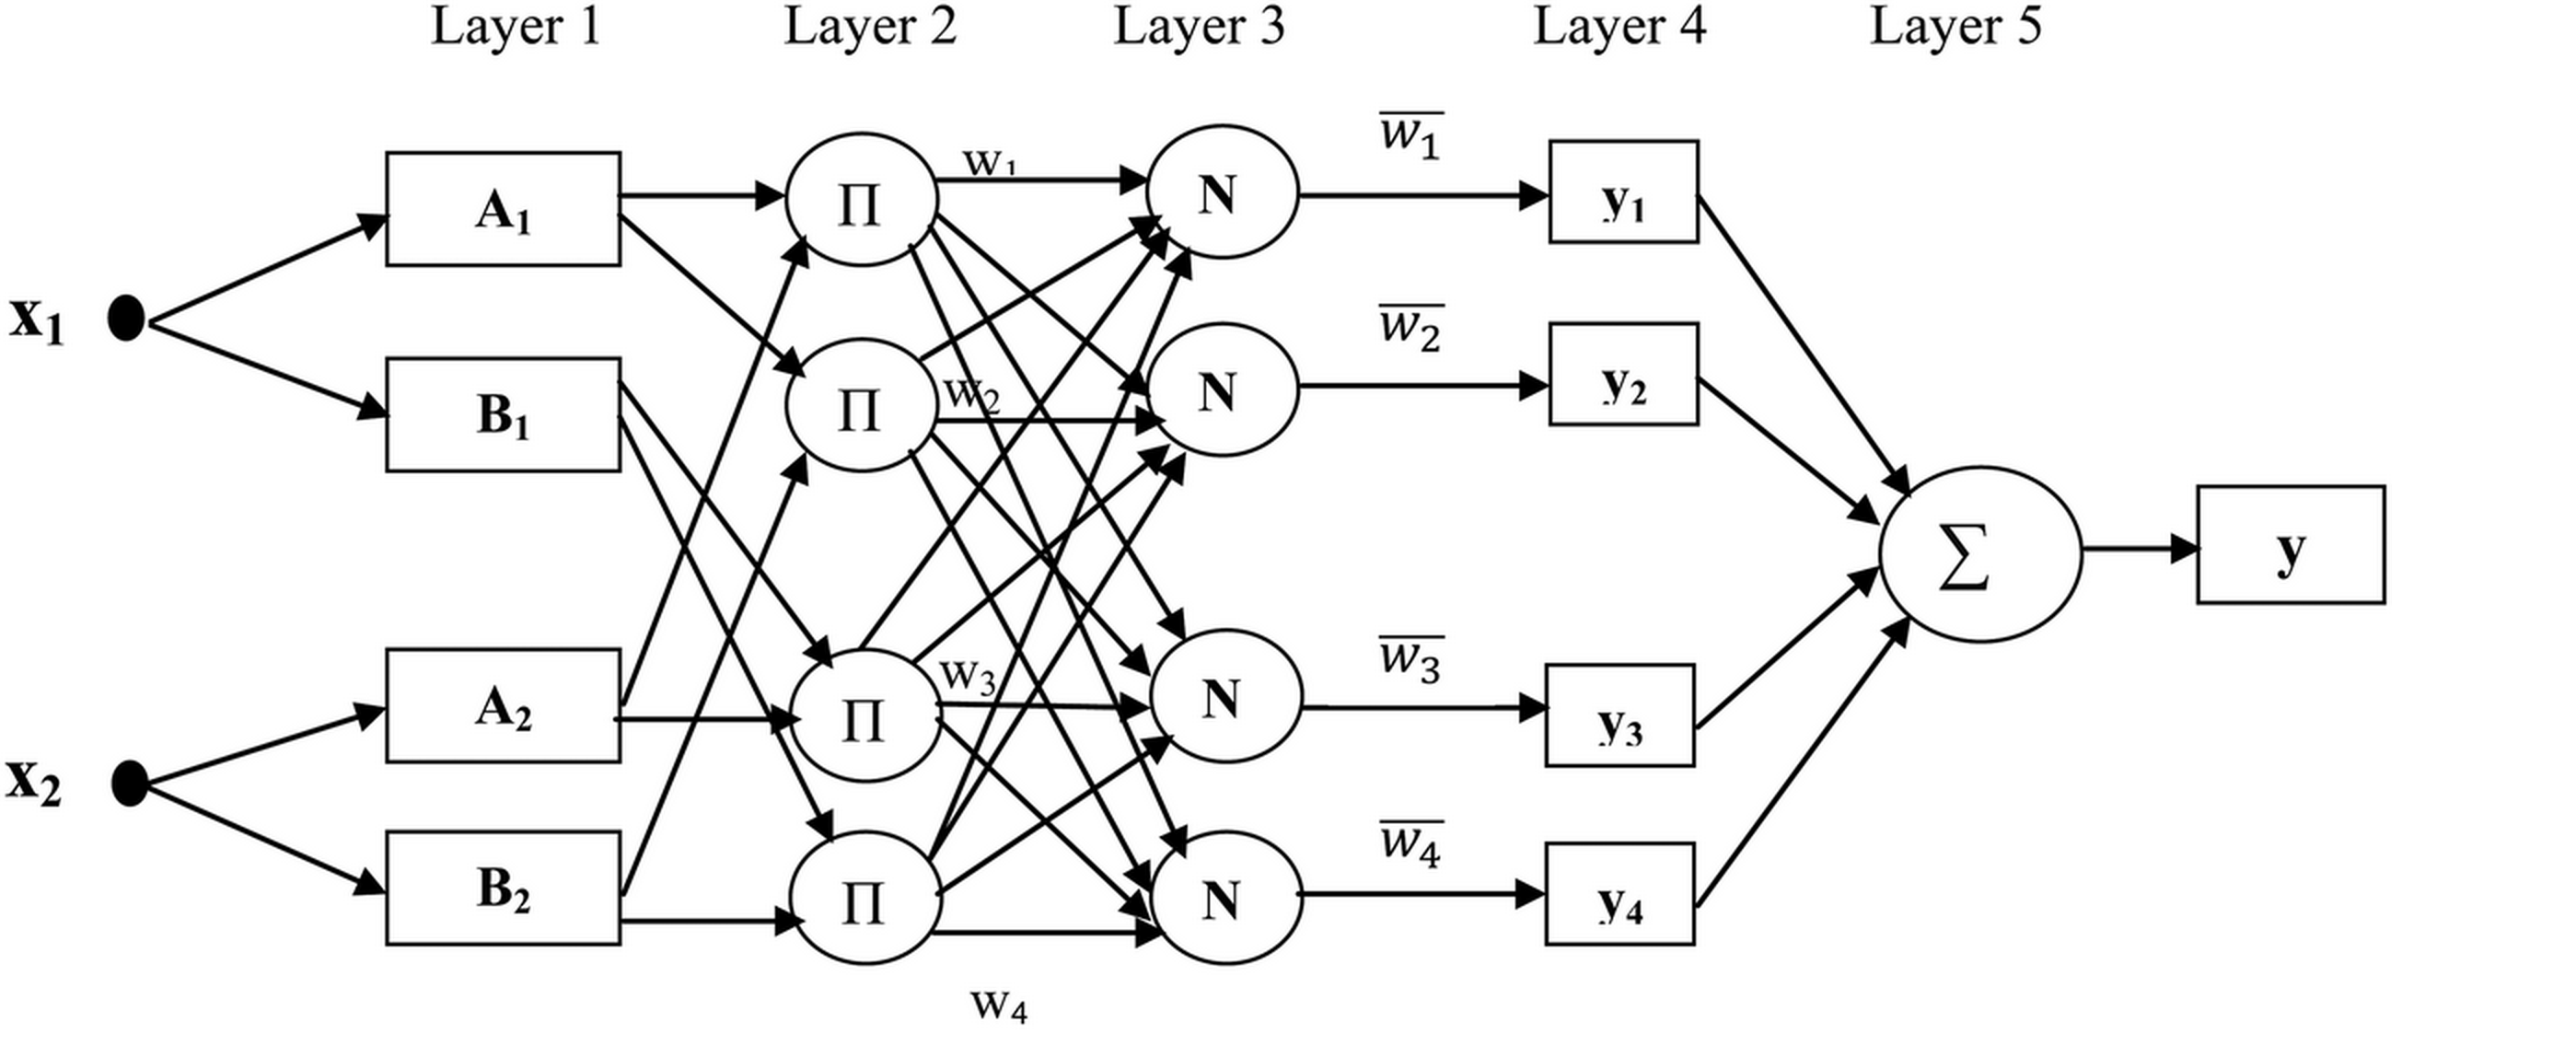
\includegraphics[width=1\textwidth ]{img/model/gnn_fuzz}      
        \caption{Annotation Distribution - Relevant to Food Security}
        \label{fig:gnn_fuzz}
\end{figure}





\section{Data Preprocessing}
\label{dataprocessing}

Before feeding the data to the Fuzzy Interfere System we analysed and cleaned the data. The representation of the data is of great importance in order to assist ANFIS in learning the relevant patterns. In a first instance we had to mach both the time series of the twitter data with the time series of the price data. The markets are closed during weekends and national holidays, hence we had to remove such instances from the twitter data. Given the sparsity of the datasets available for commodities we were forced to hand selected quotes from different markets. We observed that some of them had different closing days i.e. some markets considered a day a holiday, some others not. For wheat and cattle we removed the 12/11/12 and the 8/10/12 which are the veteran day and the columbus day respectively in order to match the price data of milk.  Secondly, we proceeded to interpolate zero values. Some of the price data-sets showed values of zero on days which were neither weekends nor holidays. Similarly, the twitter archive did not contain  twitter data for some time periods. We linearly interpolated such missing values by solving and approximation to the partial differential equations \cite{john2012}.  Fuzzy Interference Systems expect an input of a unit interval i.e. between 0 and 1. We hence normalised the data as illustrated in Equation 4.1. Min and Max are the lower and upper bounds of data set where $\alpha$ is a small constant we introduced to avoid zero divisions. It is is generally advised to normalise the data else the training algorithm might loose its sensitivity towards smaller scaled features. 

\begin{equation} \label{eq:solve}
\overline{ y } = \frac{x - min}{max - min}  + \alpha \end{equation}


Lastly we performed a scaling of the data which is in accordance of our objective, namely to be more sensitive to long-term than to short-term fluctuations. As we can see in Figure 4.1 a) there are some extreme price increases and drops. By applying the Hodrick-Prescott decomposition \cite{edward81} filter we receive a distribution which is more normal by avoiding such outliers. Additionally the Figure 4.1 illustrates nicely the characteristics of commodities, namely that it's mostly driven by small price changes. 






\begin{figure}[ht]
        \centering
        \begin{subfigure}[b]{0.5\textwidth}
                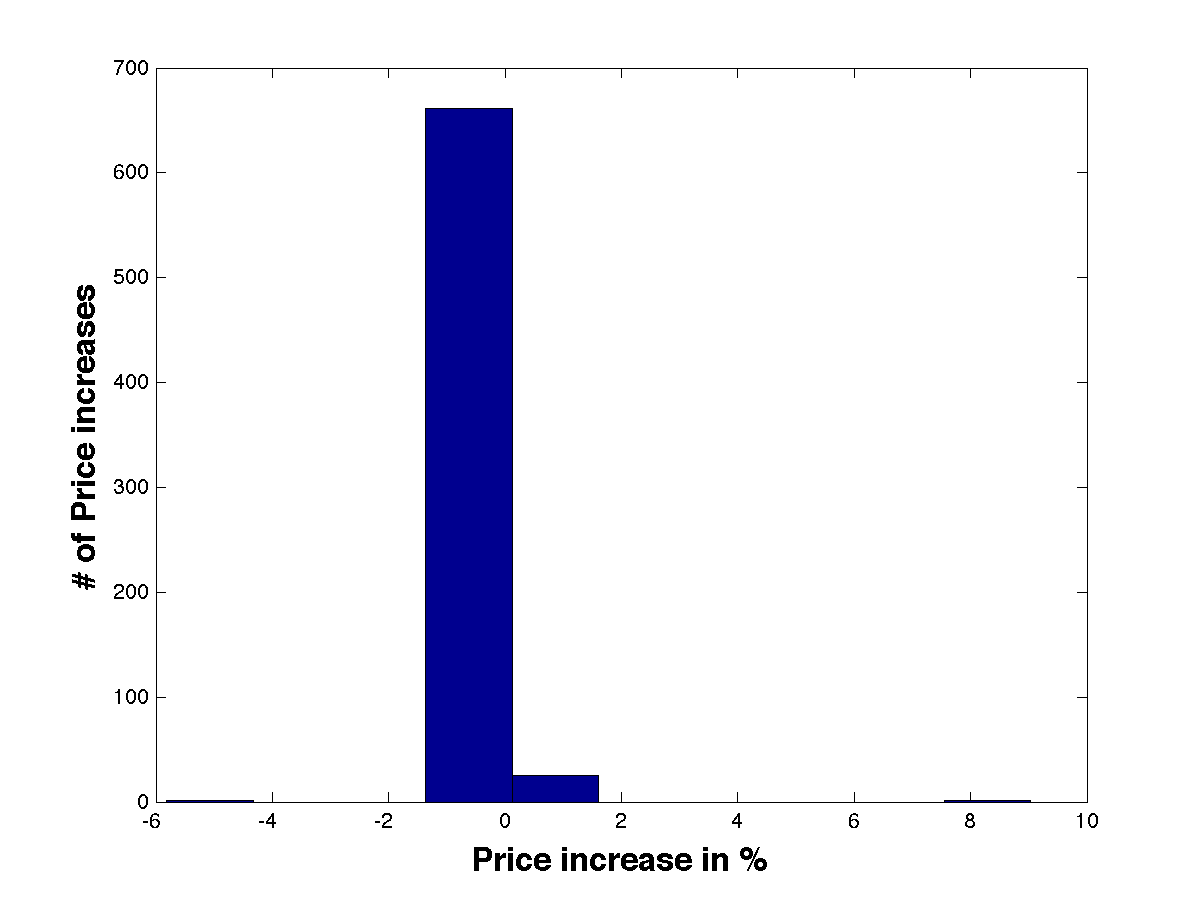
\includegraphics[width=\textwidth]{img/model/p_increase_n_log}
                \caption{Price Increase Distribution without Scailing}
                \label{fig:u_linear}
        \end{subfigure}%
        ~ %add desired spacing between images, e. g. ~, \quad, \qquad, \hfill etc.
          %(or a blank line to force the subfigure onto a new line)
        \begin{subfigure}[b]{0.5\textwidth}
                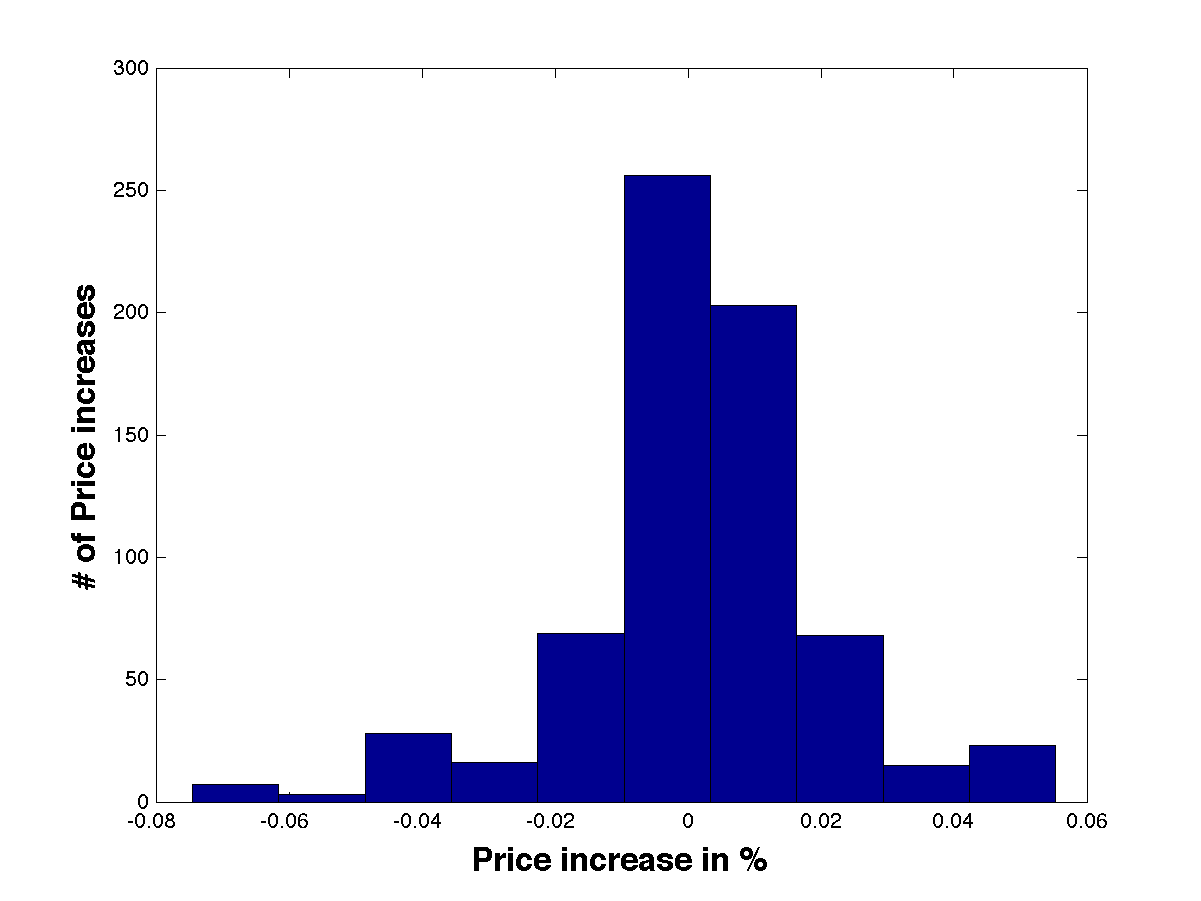
\includegraphics[width=\textwidth]{img/model/p_increase_w}
                \caption{Price Increase Distribution with Scailing}
                \label{fig:u_log}
        \end{subfigure}
        ~ %add desired spacing between images, e. g. ~, \quad, \qquad, \hfill etc.
          %(or a blank line to force the subfigure onto a new line)

      
        \caption{Volume of Tweets per Keyword and per Category}\label{fig:distribution}
\end{figure}





\section{Training the Model}

For training ant testing our model we choose the time period 03.01.2012 - 26.09.2014. We thought of numerous ways to test and train our model. Different approaches have been suggested by Ibeling Kaastra \cite{Kaastra96designinga}. Most commonly the data is split into a train set, validation set and lastly a test set. The model is trained once in a batch fashion and used for all future predictions. Such an approach can be dangerous particularly when one considers historical data reaching far into the past. Market conditions might have been different then and might not apply for future predictions. Choosing a particular time frame can be a bad idea as well. Consider the training data only exhibiting an upwards trend the model will then not generalise well for declining prices. Yao et al. \cite{Yao00acase} proposed to use statistical methods to investigate the best time period for training the network. However to make any statistically significant claims we need more then 2.5 years of historical data. Lastly Ibeling Kaastra describes a method called the walk-forward or sliding window approach. This approach involves creating overlapping sets of train and test data. Each set is moved forward through the time series to test the robustness of the model. This framework addresses the concern raised regarding including data form far in the past that might not reflect the current market conditions and is widely used for commodity predictions. We decided to apply a variant of the sliding window approach and train or model in an online fashion. Given the limited amount of data we choose not to exclude any data from future prediction, however to be able to adapt to new market conditions we increase the training and validation window as we move along the time line. To achieve a good generalisation the proportion of train and validation set always remain the same as we add additional data. We used the first 50 \% of the data to train the model. From that set we excluded 15 \% for validation purposes. These values were obtained empirically. 



\section{Methodology for Forcasting with Fuzzy Logic}

The goal of our research is to predict the price of a commodity in the future. The prediction model takes different features $y_t - y_{t-M+1}$ and an input. The problem of predicting the future value $y_{t_1}$ can be formulated as: 


\begin{equation} \label{eq:solve}
y_{t + 1} = fp(y_{t}, y_{t-1}, y_{t-M+1})
 \end{equation}

where M is the number of features and fp is our fuzzy prediction model. Consider the case where we predict $y_{t +4}$ , so four days into the future. A recursive way would be to predicted values $y_{t+2}$ and $y_{t+3}$ and then use them as regressors in predicting $y_{t +4}$. However this approach accumulates prediction errors. The further the prediction value is the more prediction outputs are used as regressors. We deviate from this approach by building a direct prediction model, so for each prediction horizon one direct model. 

Translating the Equation 4.9 into the fuzzy system a prediction would take the following form: \\

\centerline {$ \textbf{IF} <  y_t  \in High> \textbf{AND} < y_{t-1} \in Medium > \textbf{THEN} <  y_{t+1} \in Increase > $} 


where High, Medium and Increase are Fuzzy Sets. We measure the difference between the actual value and the predicted value by computing the Root Mean Square Error (RMSE) defined in Equation \ref{eq:rmse}. It is an aggregation of all prediction errors for different time stamps. As RMSE is scaled dependent it is important that the input and output variables among different commodities are normalised to be able compare the results across the different products. 


\begin{equation} \label{eq:rmse}
RMSE = \sqrt{\frac{1}{n}\sum_{t=1}^{n} (y_i -  \overline{y_i})^2}
 \end{equation}





\section{Parameters}

All experiments have been conducted with the following parameters



\begin{itemize}
  \item Input membership function: \indent Gaussian
  \item Output membership function: \indent Linear
  \item FIS generator: \indent Fuzzy C-Means 
  \item Training epochs: 500
  \item Initial step size: 0.01
  \item Step size decrease rate: 0.9
  \item Step size increase rate: 1.1
  \item Retrain rate: 28 days
  \item Initial training window size: 50 \%
  \item Segmentation: 85 \% Training , 15 \% Validation 
\end{itemize}



\section{Benchmark Model}

\subsection{Input Model}

Yao et al. [ref] suggests that the market can be categorised using the major trend the intermediate trend and the minor trend. Where the major trend lasts more then a year, intermediate trends are anything between 3 weeks to three months. We capture such trends by taking the moving average of 1 week, 2 weeks and 1 month respectively. Given the limited time frame we chose to exclude major trends. We further consider all days preceding the horizon 30 days into the past as potential features. Moving averages are known to remove the day to day instability and extract the underlying trend.


\begin{table}[H]
\centering
\begin{tabular}{ |c|c|c| } 

 input \# & name & value \\ 
  \hline
 1 & D1 & x \\ 
 2 & D2 & x -1 \\ 
 :& : & : \\ 
  :& : & : \\ 
  :& : & : \\ 
  30 & D30 & x - 29\\ 
  31 & W1 & $\mu(]x-7;x])$ \\ 
  32 & W2 & $\mu(]x-14;x])$ \\ 
  33 & M1 & $\mu(]x-30;x])$ \\ 
 

\end{tabular}
\caption{Input Model: Benchmark Prediction}
\label{tab:abc}
\end{table}


\subsection{Feature Selection}
\label{featSel_bench}


The objective here is to find the most significant features among the 33 in our input model in order to decrease the complexity and lastly improve the prediction accuracy of our model.  To investigate the relevance we used the Relieff algorithm []. We measure the most significant features with respect to the horizon of 4 days, 7 days and 14 days. Furthermore we consider  three different commodities, wheat (w), beef (b) and milk (m). The configuration in the Table \emph{w-4} refers to wheat with a prediction horizon of 4 days. The most significant features are  1.) $\phi_1$ : $D30$ , 2.) $\phi_2$ : $D29$,  3.) $\phi_3$ : $D28$, 4.) $\phi_4$ : $W1$ , 5.) $\phi_5$ : $D27$ and 6.) $\phi_6$ : $D26$.

The numbers in the table refer to the relative importance of the feature for a specific configuration. It is interesting to observe that the Relieff consistently suggested the same features irrespectively of the commodity type and the prediction horizon. This gives us a strong confidence in the relative importance of the prediction task at hand, as it generalises well over different models i.e. horizons and also different commodities. We can see that the values follow a clear trend. With an increasing horizon the features lose its importance as the prediction task becomes more and more challenging. 


For our prediction task we consider the top 10 features. This value was empirically evaluated and is a trade off between computational complexity and accuracy. Better prediction accuracy is expected for values greater the 10 however the search will become too exhaustive.  Those additional feature ($\phi_7 - phi_10$ not displayed in Table \ref{tab:feat_mod1}  are for most commodities and horizons the same but ranked in different orders depending on the prediction task. Interestingly D25, D24, D23 and W2 rank highly along the other values in Table \ref{tab:feat_mod1} which are all placed in the intermediate past. This observation suggests that models based on the intermediate past poses more predictive power and outperform strategies based on features in the recent past. Robert Novy - Marx also observed this effect and investigated the hypothesis in \cite{iuj11}. Indeed models with intermediate variables tend to outperform such only considering recent values. A possible explanation mentioned in the paper is that such variable best captures the momentum of a commodity. 




\begin{table}[H]
\centering
\begin{tabular}{ |p{2cm}|p{1cm}|p{1cm}|p{1cm}|p{1cm}|p{1cm}|p{1cm}|p{1cm}|p{1cm}|p{1cm}| }
  \hline
 Feature & w-4 & b-4 & m-4 & w-7 & b-7 & m-7 & w-14 & b-14 & m-14   \\
 \hline

 $\phi_1$ & 0.0624   & 0.0212   & 0.0310 &  0.0586  & 0.0197 & 0.0300 & 0.0487 & 0.0155 & 0.0271\\
  \hline
  $\phi_2$ & 0.0558 & 0.0193 & 0.0281 & 0.0513 & 0.0175 & 0.0268 & 0.0411 & 0.0132 & 0.0237 \\
  \hline
  $\phi_3$ & 0.0495 & 0.0174 & 0.0253 & 0.0444 & 0.0153 & 0.0236 & 0.0343 & 0.0111 & 0.0205 \\
  \hline 
  $\phi_4$ & 0.0440 & 0.0157 & 0.0227 & 0.0388 & 0.0135 & 0.0209 & 0.0291 & 0.0093 & 0.0179 \\
  \hline 
  $\phi_5$ & 0.0434 & 0.0156 & 0.0225 & 0.0381 & 0.0133 & 0.0206 & 0.0283 & 0.0091 & 0.0175 \\
  \hline
  $\phi_6$ & 0.0378 & 0.0138 & 0.0198 & 0.0324 & 0.0114 & 0.0178 & 0.0231 & 0.0074 & 0.0149 \\
  \hline
 \end{tabular}
\caption{Feature Selection: Benchmark Prediction}
\label{tab:feat_mod1}
\end{table}



\subsection{Results}

The prediction results across different time horizons are highlighted in Figure \ref{fig:res_1}. To give an example of the interpretation of the model the results are obtained by applying the model describe in Section 4.5. The features used in the form of $y_{t-2}$ are the top 10 obtained from the feature selection process. If the prediction task is to predict $y_{t+3}$ and for illustration purposes we assume today is Monday, then the prediction goal translates to approximating the true value on the following Thursday. Assuming the feature selection process yields $y_{t-1}$  and $y_{t-1}$ this corresponds to using the price on the previous Sunday and Saturday. Finally our model with two membership functions High and Low gives us the following Fuzzy Model. \\

\centerline {$ \textbf{IF} <  Sunday \in High> \textbf{AND} < Saturday \in Low > \textbf{THEN} <  Thursday \in 0.67 > $} 

The output is a numerical value and not a class. 

 Looking at the results ANFIS performs exceptionally well for day to day predictions and as expected decreases its performance as the horizon increases. The commodity beef seems to be the eassiest prediction task and further analysis will clearly show why.   We observe that RMSE linearly increases over the time period until prediction horizon 20. Prediction accuracy rapidly decreases and becomes unstable from then onwards.  

To analyse the results in more detail and to put the RMSE into context  we turn our attention towards Figure \ref{fig:wheat_1} \ref{fig:beef_1} \ref{fig:milk_1}. For all three commodities the predictions within one week are extremely accurate. We can now also observe why beef had the lowest RMSE among the three commodities. Beef follows a clear upwards trend. Such long lasting motions are much easier to predict and as discussed in Section Feature Selection our input variables from the intermediate past perform exceptionally well if there is a clear underlying motion. 

 For the model $y_{t+14}$ and $y_{t+20}$  ANFIS clearly overestimates a decrease and increase in price but still manages to captures the underlining trend. On the other hand Figure \ref{} \ref{} strongly approximates the observed pattern in the training sample explaining the strong deviation from the actual prediction. The only commodity excluded from this behaviour is beef due to it's strong underlying motion. Better predictions can be expected by considering different training samples. 






\begin{figure}[H]
        \centering
         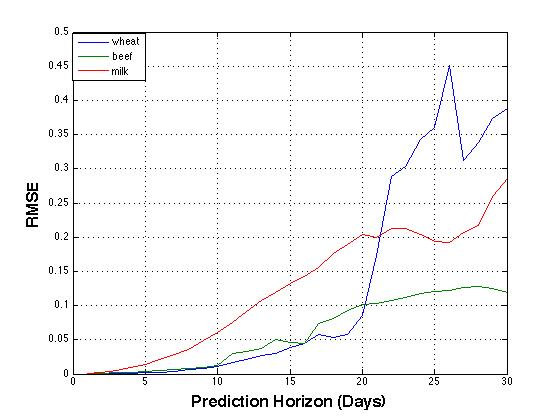
\includegraphics[width=1\textwidth ]{img/model/prediction_days_1}      
        \caption{Prediction Accuracy - Benchmark }
        \label{fig:res_1}
\end{figure}









\begin{figure}
        \centering
        \begin{subfigure}[b]{0.5\textwidth}
                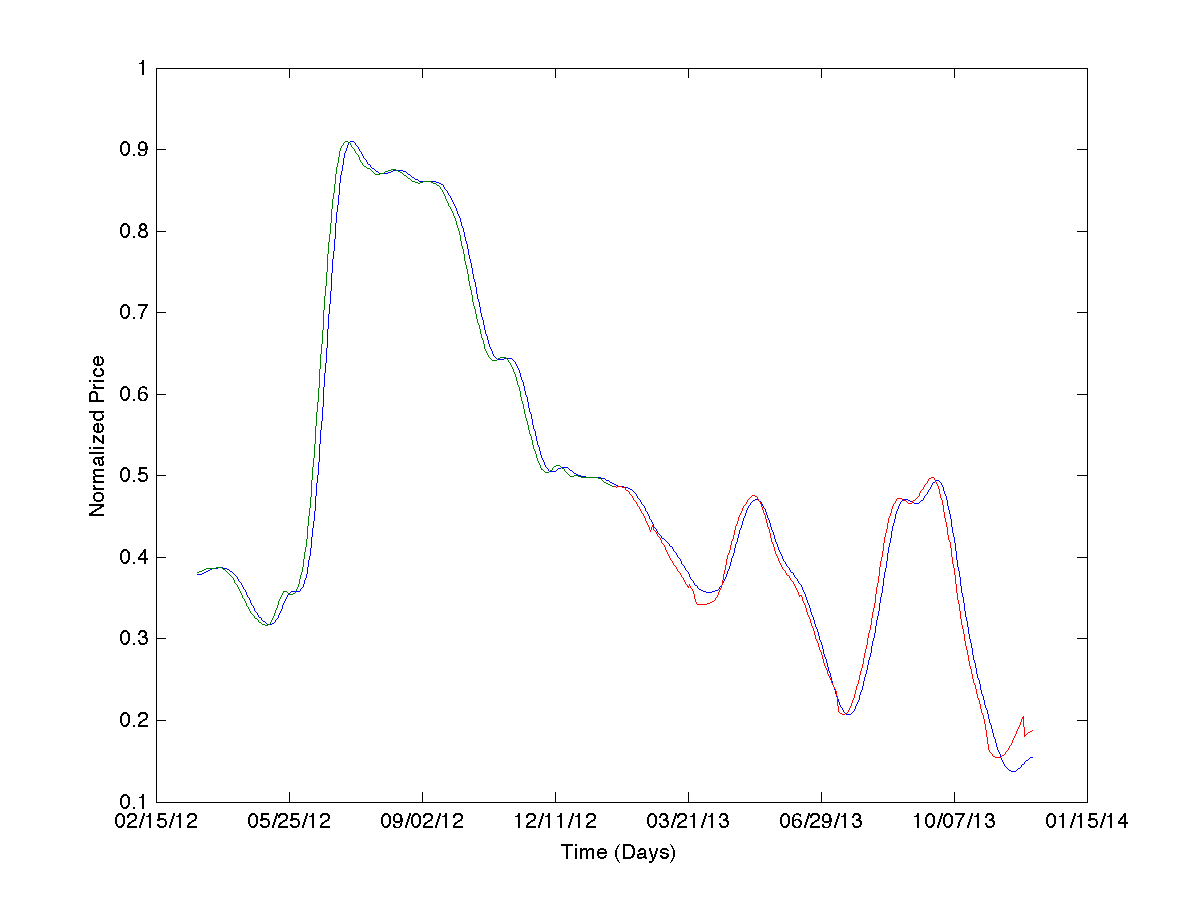
\includegraphics[width=\textwidth]{img/model/wheat/pred_4}
                \caption{4 Day Horizon - RMSE 0.0012 }
                \label{fig:gull}
        \end{subfigure}%
        \begin{subfigure}[b]{0.5\textwidth}
                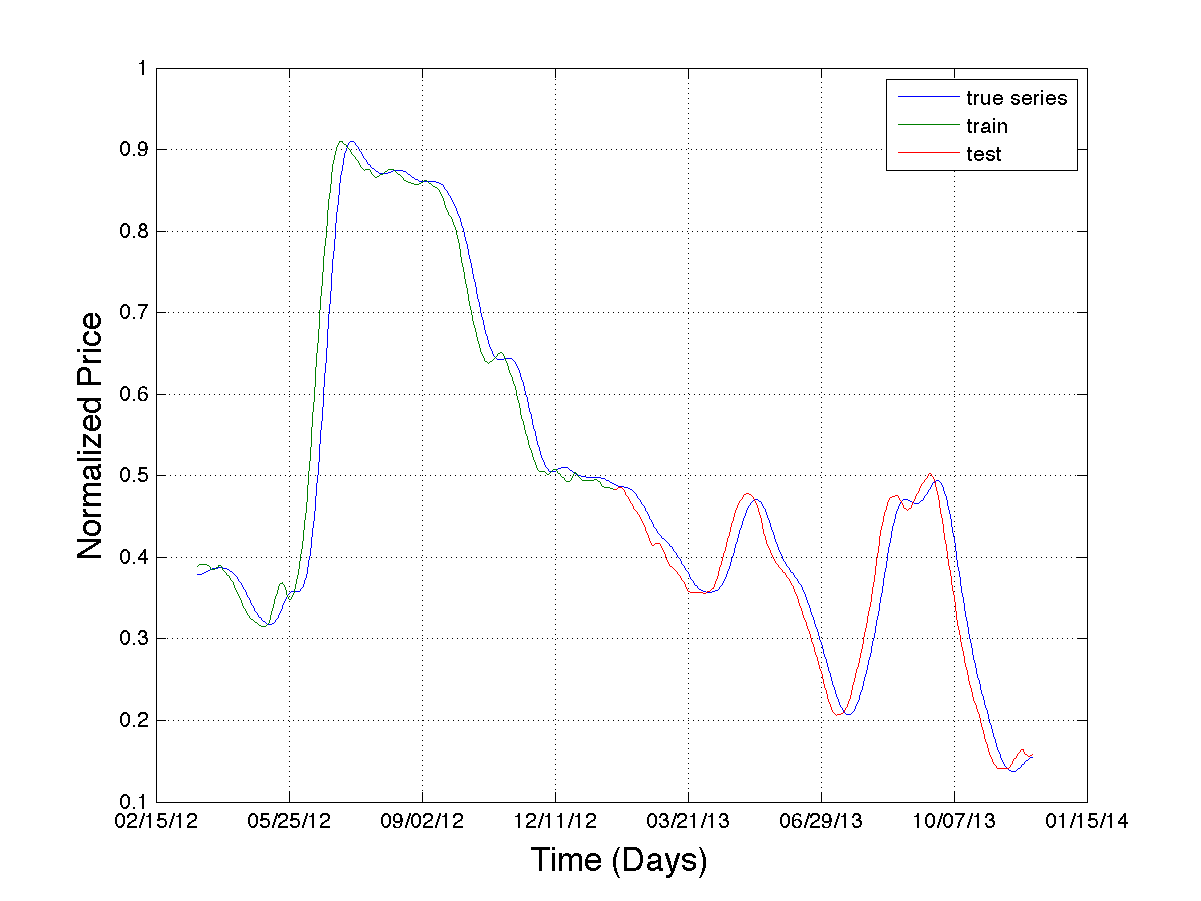
\includegraphics[width=\textwidth]{img/model/wheat/pred_7}
                \caption{7 Day Horizon - RMSE 0.0047}
                \label{fig:tiger}
        \end{subfigure}
       
       \hfill
       
        \begin{subfigure}[b]{0.5\textwidth}
                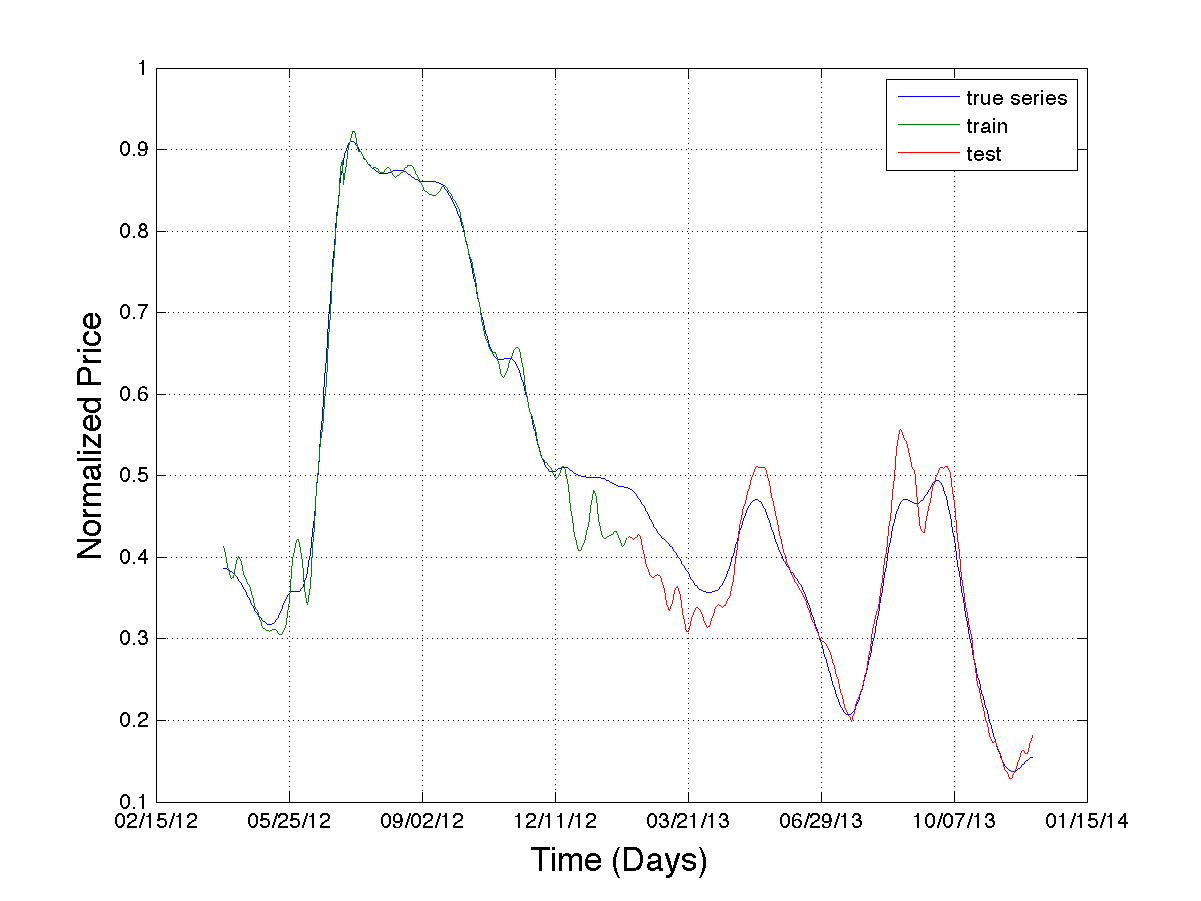
\includegraphics[width=\textwidth]{img/model/wheat/pred_14}
                \caption{14 Day Horizon - RMSE 0.0353}
                \label{fig:mouse}
        \end{subfigure}%
         \begin{subfigure}[b]{0.5\textwidth}
                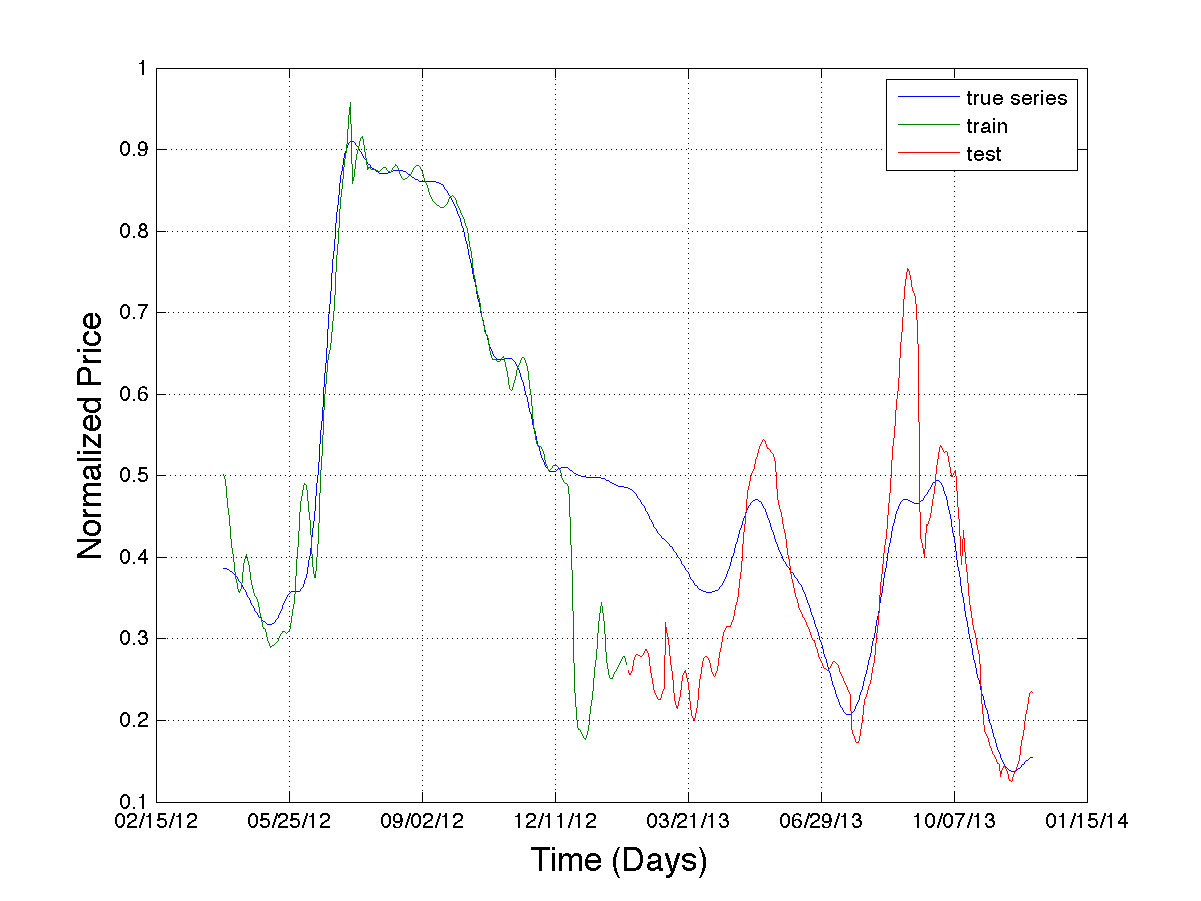
\includegraphics[width=\textwidth]{img/model/wheat/pred_20}
                \caption{20 Day Horizon - RMSE  0.1031}
                \label{fig:mouse}
        \end{subfigure}
        \caption{Benchmark Prediction Wheat}
        \label{fig:wheat_1}
\end{figure}





\begin{figure}
        \centering
        \begin{subfigure}[b]{0.5\textwidth}
                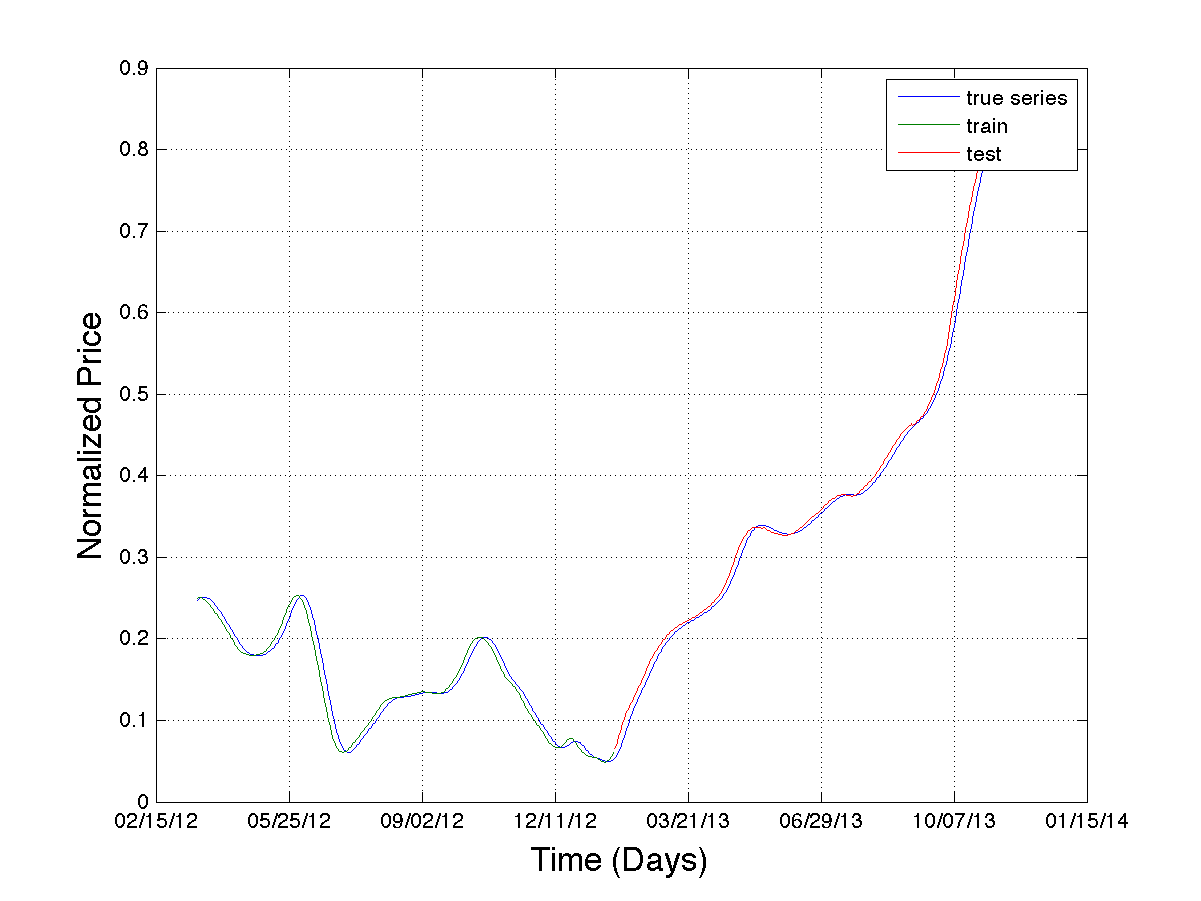
\includegraphics[width=\textwidth]{img/model/beef/pred_4}
                \caption{4 Day Horizon - RMSE 0.0027 }
                \label{fig:gull}
        \end{subfigure}%
        \begin{subfigure}[b]{0.5\textwidth}
                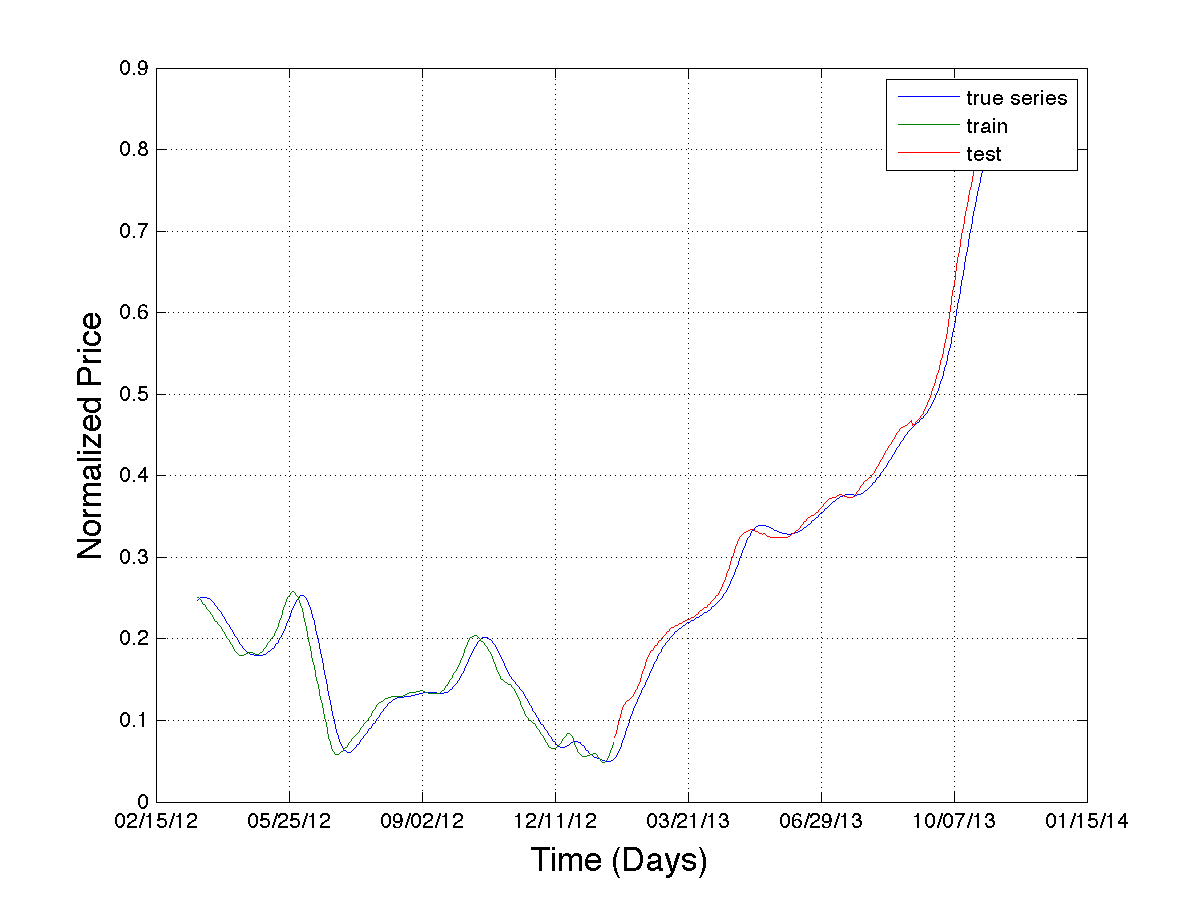
\includegraphics[width=\textwidth]{img/model/beef/pred_7}
                \caption{7 Day Horizon - RMSE 0.0066}
                \label{fig:tiger}
        \end{subfigure}
       
       \hfill
       
        \begin{subfigure}[b]{0.5\textwidth}
                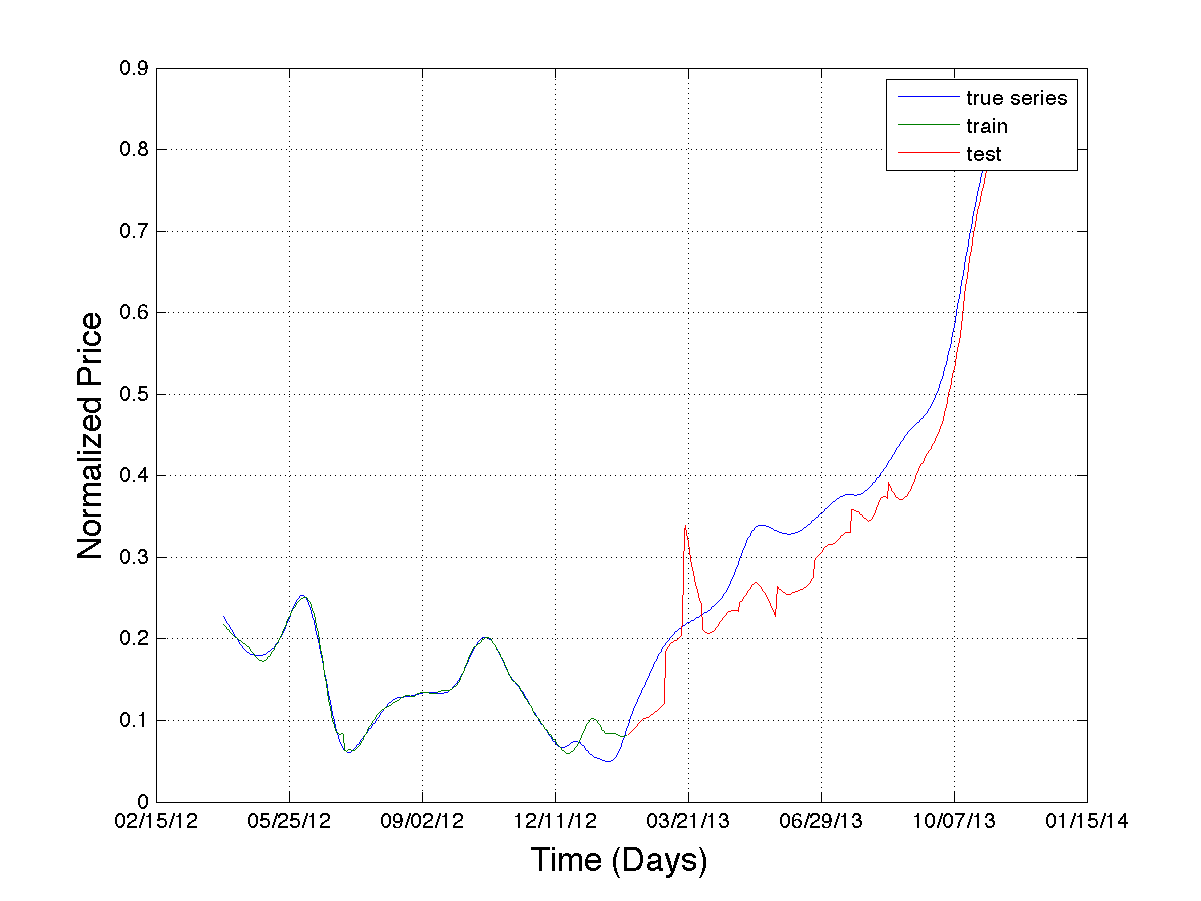
\includegraphics[width=\textwidth]{img/model/beef/pred_14}
                \caption{14 Day Horizon - RMSE 0.0508}
                \label{fig:mouse}
        \end{subfigure}%
         \begin{subfigure}[b]{0.5\textwidth}
                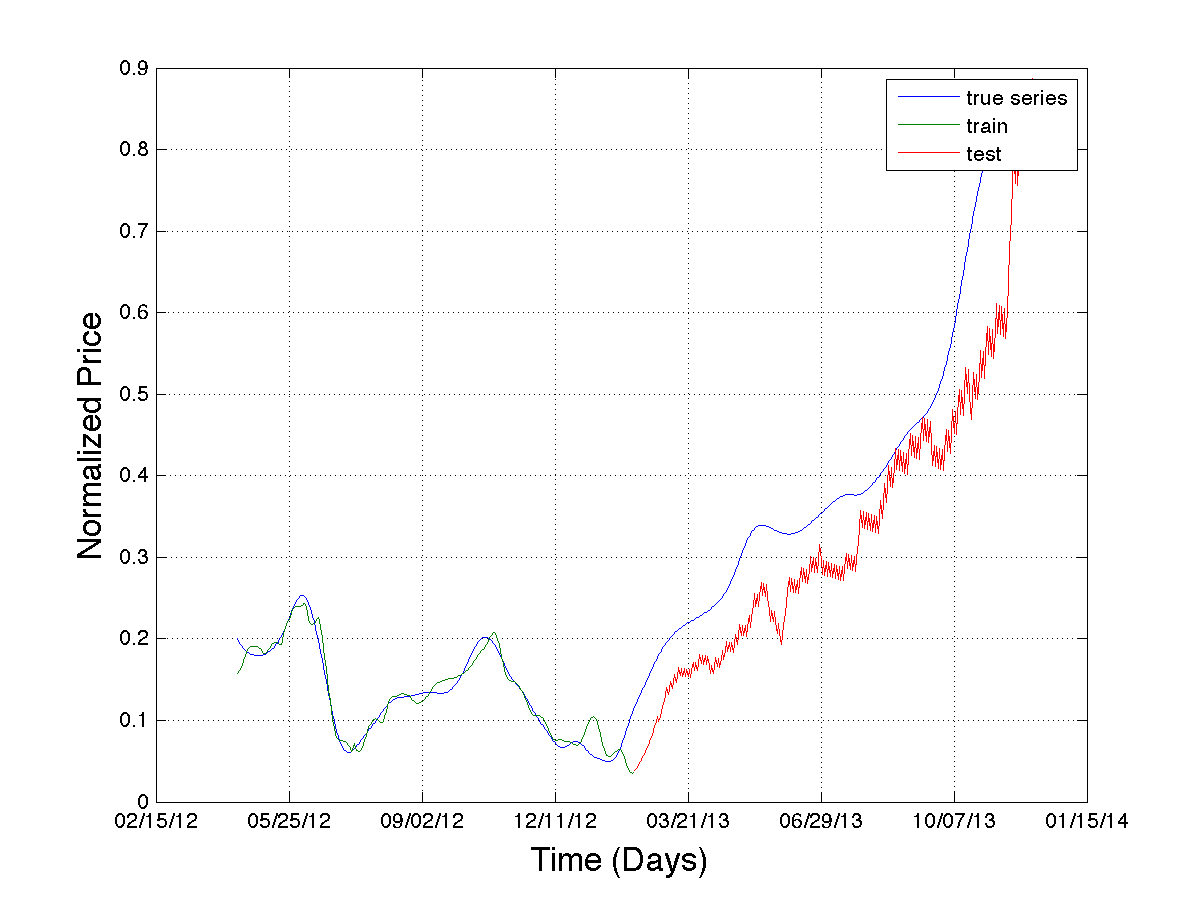
\includegraphics[width=\textwidth]{img/model/beef/pred_20}
                \caption{20 Day Horizon - RMSE 0.1013}
                \label{fig:mouse}
        \end{subfigure}
        \caption{Benchmark Prediction Beef}
        \label{fig:beef_1}
\end{figure}




\begin{figure}
        \centering
        \begin{subfigure}[b]{0.5\textwidth}
                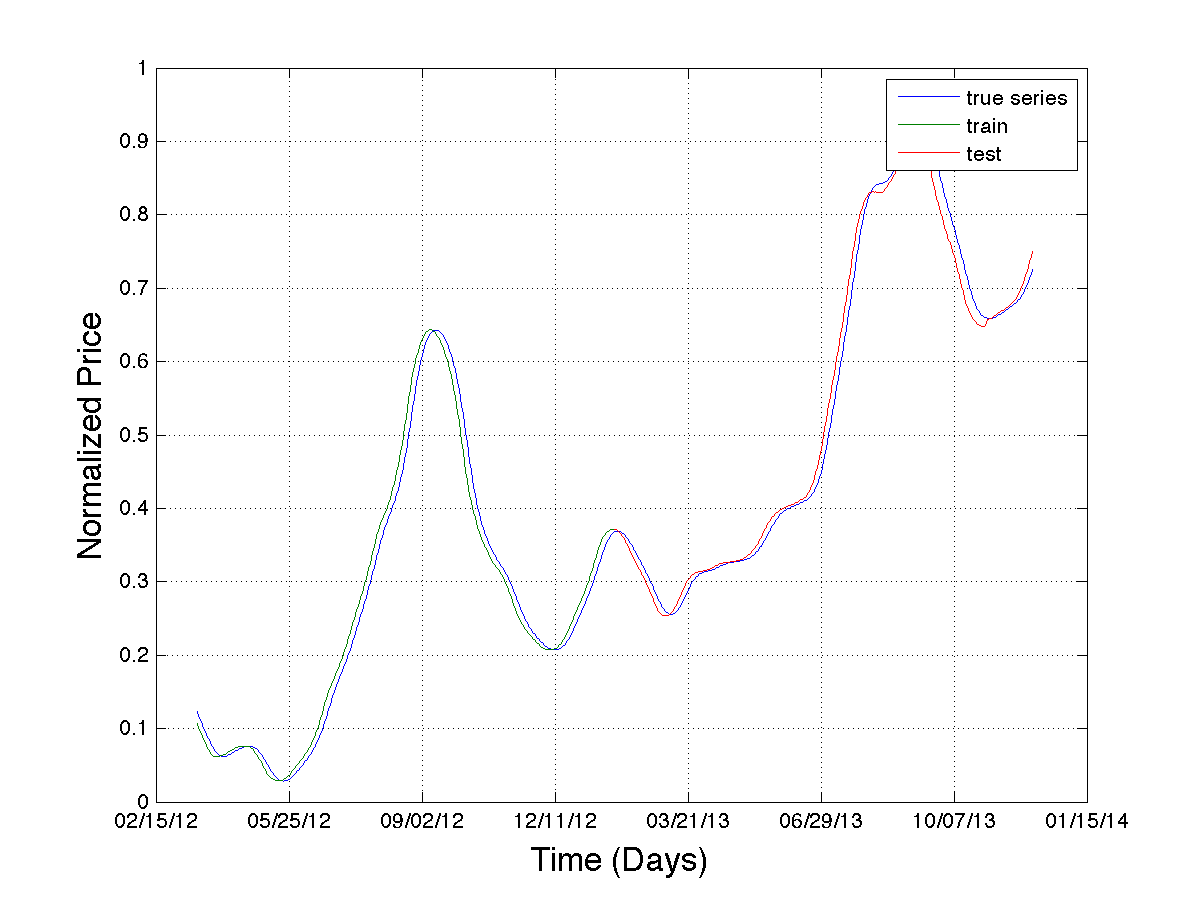
\includegraphics[width=\textwidth]{img/model/milk/pred_4}
                \caption{4 Day Horizon - RMSE 0.0088}
                \label{fig:gull}
        \end{subfigure}%
        \begin{subfigure}[b]{0.5\textwidth}
                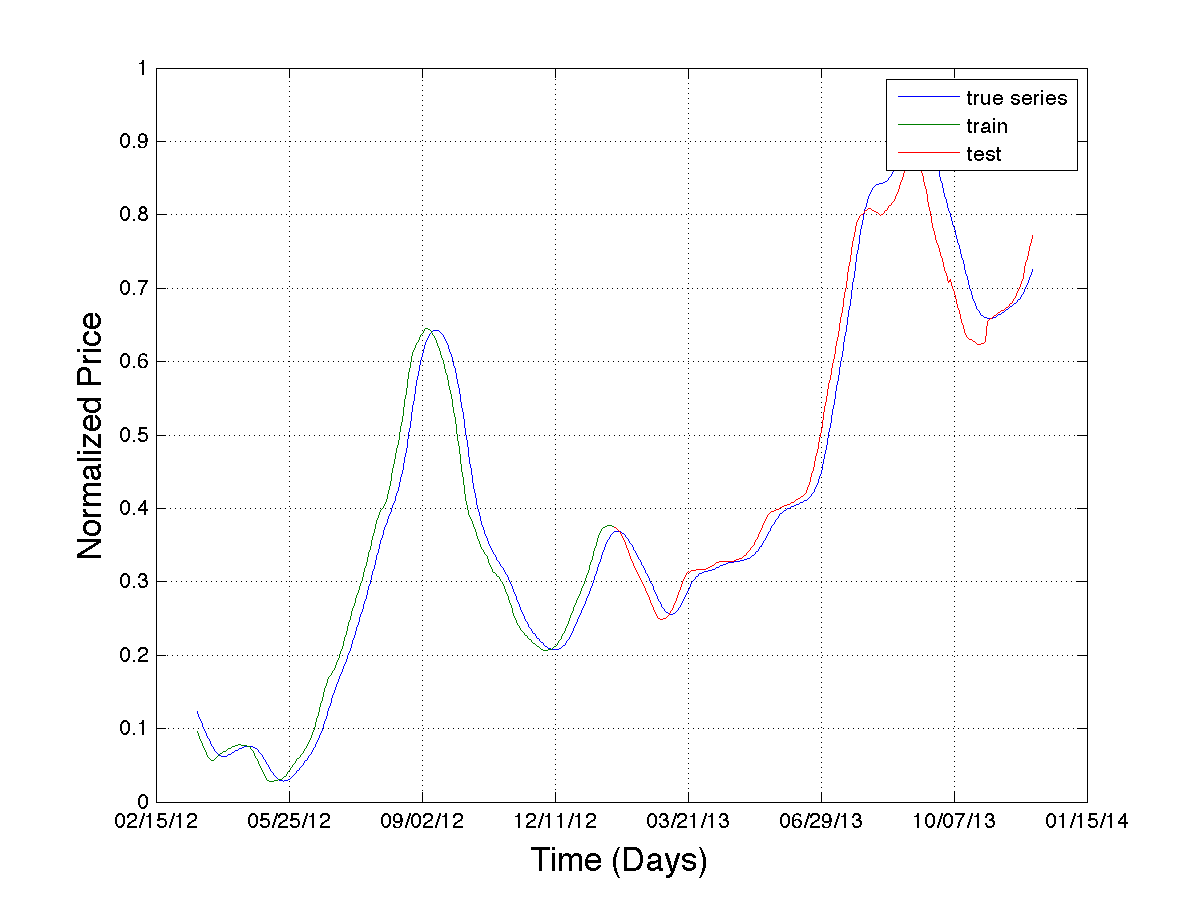
\includegraphics[width=\textwidth]{img/model/milk/pred_7}
                \caption{7 Day Horizon - RMSE 0.0286 }
                \label{fig:tiger}
        \end{subfigure}
       
       \hfill
       
        \begin{subfigure}[b]{0.5\textwidth}
                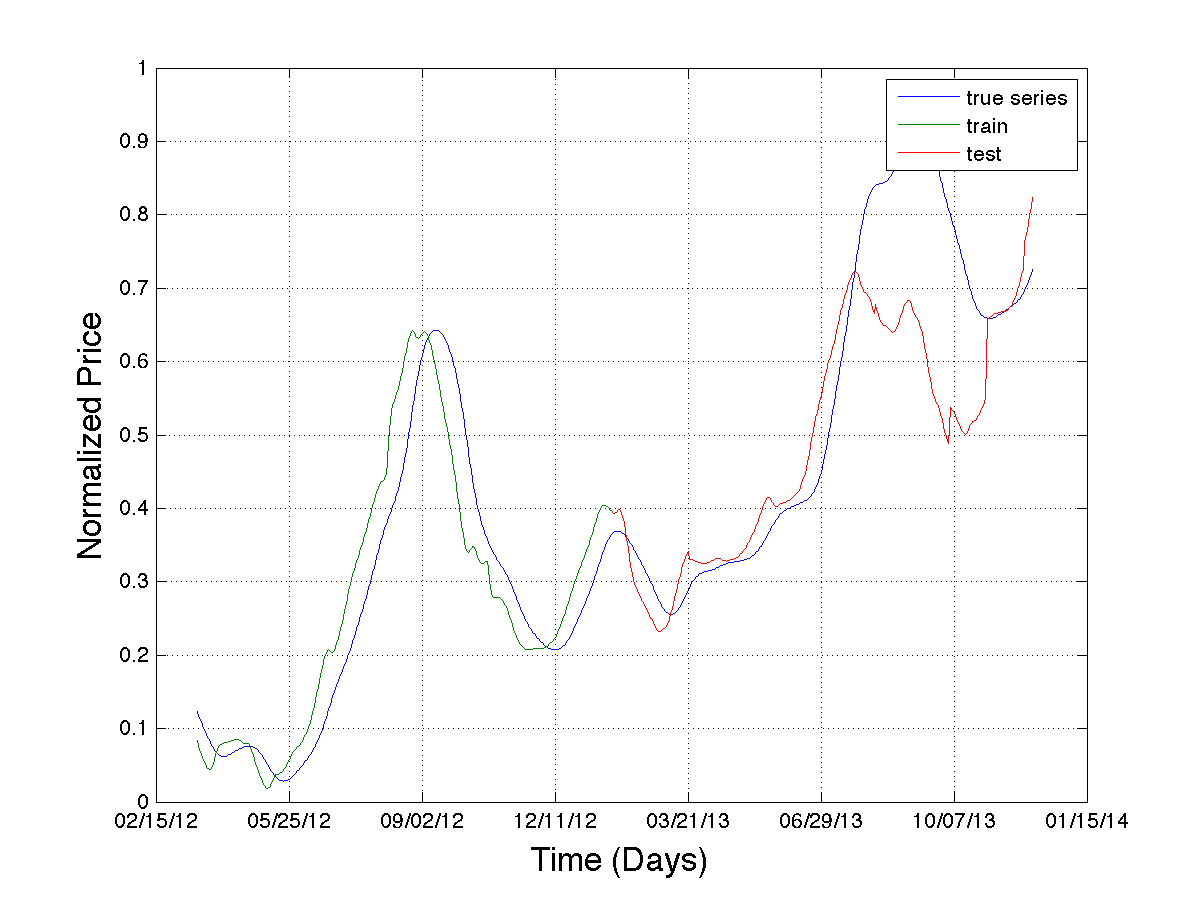
\includegraphics[width=\textwidth]{img/model/milk/pred_14}
                \caption{14 Day Horizon - RMSE 0.1185}
                \label{fig:mouse}
        \end{subfigure}%
         \begin{subfigure}[b]{0.5\textwidth}
                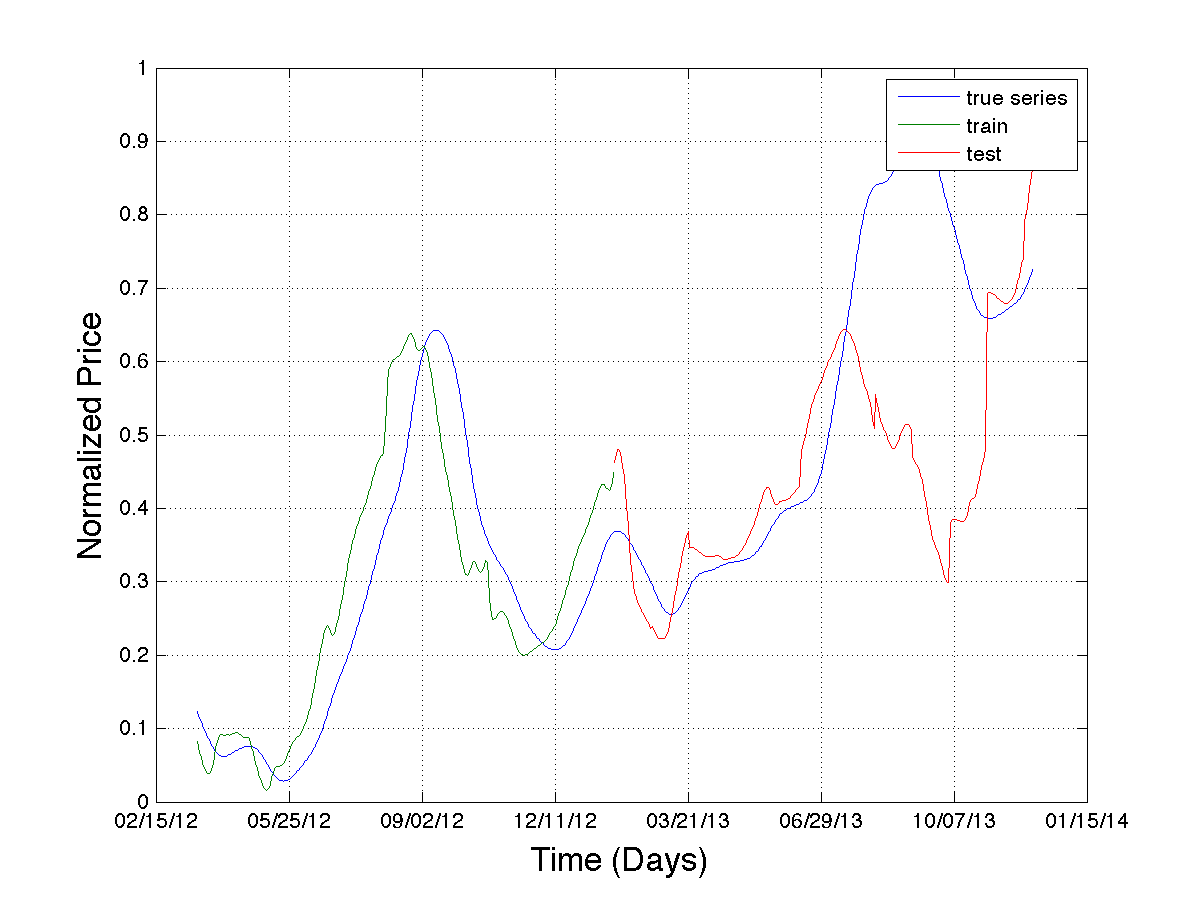
\includegraphics[width=\textwidth]{img/model/milk/pred_20}
                \caption{20 Day Horizon - RMSE 0.2039}
                \label{fig:mouse}
        \end{subfigure}
        \caption{Benchmark Prediction Milk}
        \label{fig:milk_1}
\end{figure}











\clearpage

\section{Social Media Model}

\subsection{Input Model }

Xue Zhanga et al. found that twitter conversation correlates and is even predictive of financial market movements. They measured the attention of a given subject by aggregating the daily volume. In Section \ref{corr_results} we investigated if such a correlation is present and concluded that for most commodities no such linear relationship exists. We however still include the social attention as a possible feature since it might prove to be useful in form of a lagged variable (i.e. that the volume 4 days ago  correlates to the commodity price of today). We consider social attention on different granularities  by measuring the volume of the category, subcategory and the product \ref{food_lex}. We further include products which are not part of a subcategory but show a strong linear relationship with the predicted commodity (i.e. we consider goat as a feature for beef despite it not being a related product to beef). 

 Generally speaking microblogs capture one topic due to its 140 keyword limitation. The topics can usually be inferred by capturing one or two keywords. However certain terms are more intrinsic then others i.e. the keyword \emph{IBM} can unambiguously be related to the company where as the  term \emph{break} has multiple meanings and given the context could be unrelated to a desired topic. We hence introduce the notion of contextual sensitive tweets. Tweets considered contextual sensitive match both a term in the Food Lexicon and the Predictor Lexicon. We consider the context of food price, supply, poverty and needs \ref{pred_lex}. 
 
 
 Despite having identified  a significant correlation for contextually sensitive tweets our analysis in Section \ref{conversation} concluded that the attention volatility is mostly driven by unrelated topics. Public mood states or sentiment might hence be a more valuable indicator. This intuition is supported by \cite{nofsinger05} namely that financial decisions are not uncommonly driven by emotions and mood. For the purpose of this analysis we consider different ratios of sentiment, namely the ratio between the numbers of positive and negative tweets \cite{Nguyen12}, the proportion of neutral and total tweets,  the ratio between the numbers of non-neutral and total posts \cite{Zhang09}, the ratio between the number of positive and negative discussions and lastly the ratio between the numbers of neutral and non neutral messages. 

Table \ref{tab:socio_feat} conculdes our input model. We measure the sentiment for both twitter buzz and contextually sensitive tweets. The result is an input model with 51 features. 
 

\begin{table}[H]
\centering
\begin{tabular}{ |p{3cm}|p{3cm}|p{8cm}| }



 Feature Type & Name & Value    \\
\hline
Attention & AC\# & \#Commodity   \\
\hline
Context & CP\# & \#Price f. Commodity   \\
		& CS\# & \#Supply f. Commodity  \\
		&CP\# & \#Poverty f. Commodity   \\
		&CN\# &\#Need f. Commodity  \\



  \hline
   Sentiment Ratio & SR\#& \#positive : \#negative tweets  \\
      			    & SR\# & \#positive : \#(positive + negative) tweets   \\
 			    & SR\#  & \#negative: \#(positive + negative) tweets  \\
			   &SR\#   & \#neutral : \#(positive + negative) tweets  \\
			    &SR\#  & \#(positive+negative) : \#all tweets   \\			     
			    &SR\#  & \#neutral : \#all tweets \\
                          

   


\end{tabular}
\caption{Input Model: Social Media Prediction}
\label{tab:socio_feat}
\end{table}


\subsection{Bolstering the Social Media Features}

In chapter \ref{dataprocessing} we motivated the use of a smoothing function in order to aid our goal of predicting a trend. This kind of preprocessing becomes especially important for social media data as it's characterised by an extreme day to day volatility as illustrated in Figure \ref{fig:inc_dist} . We experimented with three different smoothing techniques 1.) the weekly moving average , 2.) the monthly moving average and 3.) the Hodrick-Prescott decomposition which we previously used to smothen our price data. The effect of the smoothing functions is displayed in Figure \ref{fig:s_effect}. Where the moving average seems to have a delayed approximation of the true trend  Hodrick-Prescott decomposition shows a much exacter approximation of the underlying motion. We compared the different smoothing techniques by measuring the correlation increase of the respective smoothing functions in Table \ref{tab:smoothing_corr}. Hodrick-Prescott decomposition significantly improved the correlation between the commodity price and the sentiment features and was able to increase the correlation more then the moving average approach. 



\begin{figure}[ht]
        \centering
        \begin{subfigure}[b]{0.5\textwidth}
                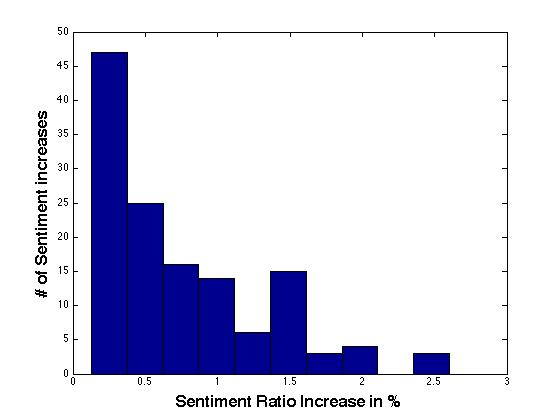
\includegraphics[width=\textwidth]{img/model/sentiment_increase}
                \caption{Price Increase Distribution of Sentiment Ratio}
                \label{fig:inc_dist}
        \end{subfigure}%
        ~ %add desired spacing between images, e. g. ~, \quad, \qquad, \hfill etc.
          %(or a blank line to force the subfigure onto a new line)
        \begin{subfigure}[b]{0.5\textwidth}
                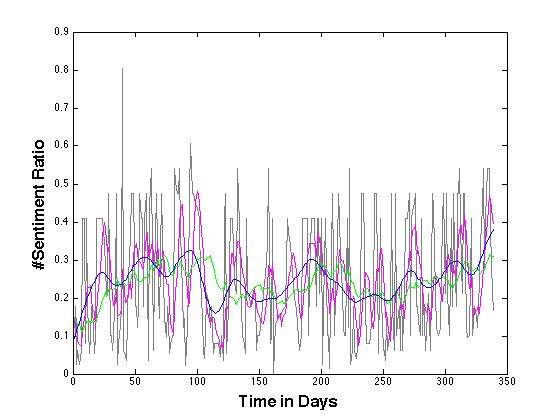
\includegraphics[width=\textwidth]{img/model/smoothing_variance}
                \caption{Smoothing functions: Past Week (Magenta), Past Month (Green), HPD (Blue)}
                \label{fig:s_effect}
        \end{subfigure}
        ~ %add desired spacing between images, e. g. ~, \quad, \qquad, \hfill etc.
          %(or a blank line to force the subfigure onto a new line)

      
        \caption{Volume of Tweets per Keyword and per Category}\label{fig:distribution}
\end{figure}





\begin{table}[h]   
\centering
 \begin{tabular}{  c  | c  | c | c }
			
    \textbf{Smoothing}  & \textbf{S1 Product} & \textbf{S2 Subcategory} &\textbf{S5 Poverty} \\
  \hline 
  &&& \\
  No Smoothing & 0.1463*  &   0.1340* &    0.1719**  \\
  
  Weekly MA &    0.2528***   & 0.1830** &   0.3111***\\

  Monthly MA &  0.2889***  & 0.1466* & 0.4847*** \\

  HPD &  0.3586 ***  &  0.2673*** &   0.5957***  \\
  

\hline 

\multicolumn{4}{c}{\null}\\

\multicolumn{4}{c}{\textbf{Significance:} p $<$ .0005 ***, p $<$ 0.005 **, p $<$ 0.05 *}\\
\hline  

\end{tabular}
\caption{Sentiment Correlation}
\label{tab:smoothing_corr}


\end{table}


We further investigated to what extend twitter lags as an indicator. If a casual relationship exists, how fast do prices react to twitter conversations? Graphically this corresponds to shifting the sentiment ratio to the left. For each social media feature (51) we measured the correlation between 1 day and 3 days lag similar to \cite{Si_exploitingtopic}. We choose a window of three days because typical non of the attention spikes showed to last longer then 3 days (Section 3.4).  The experiment was performed on all three commodities. Incase of a disagreement we solved  the tie through a majority voting. A 
 lag of 3 days clearly favoured the correlation with 44 out of 51 (0.86 \%) features and a 1 day lag for 7 out of 51 (14 \%) features. 


\subsection{Feature Selection}

For the purpose of this analysis we repeat the exercise performed in \ref{featSel_bench}. Again we try to find features that generalise well among different commodities and horizons. Unlike the price data the social media features seem to be more specific to a given task and commodity. For the top 16 features we only found 3 features that were present for all commodities and all horizons. Among the three were \textbf{1.)} the attention count of the selected products that showed a high correlation in our analysis (AC50), \textbf{2.)} the first sentiment ratio of poverty (SR32) and \textbf{3.)} the first sentiment of the subcategory (SR15). Other features that generalised well for all prediction tasks of a given commodity were 1.) the second sentiment of the subcategory (SR16), 2.) the 2nd sentiment of poverty (SR33), the fourth sentiment of poverty (SR35), the first sentiment of price (SR38), the second sentiment of supply (SR45), the sixth sentiment of supply(SR49) and lastly the attention count of another selected product that scored well in our correlation analysis (AC51). The top features for each given commodity are illustrate in Table \ref{tab:feat_mod2}.

Sentiment ratios are clearly the favoured features where only the highly selected volume counts seem to have a considerable effect. The sentiment of our contextually sensitive tweets appear to be a strong indicator of the price variance, especially the sentiment for poverty which was captured in the form of three different ratios. In \ref{an_result} we showed the peaks had the highest relevance for  discussion centered around poverty. Admittedly, it's not a decisive indicator for the quality of the feature, however it might explain why poverty features rank so highly. Similarly the three food security indicators, that have been selected by Relieff all showed a degree of relevance in our analysis. Needs had no relevance and hence it doesn't come as a surprise that it was not selected as a potential feature. It appears that Relieff successfully removes redundant features. We would for example expect needs and poverty to be similar likewise supply and price. Non of them overlap in the ratios used. Lastly, the sentiment ratios 1 and 2 seem to be more indicative then others. They only include information about the ratio of positive tweets [why is that the case????]


\begin{table}[H]
\centering
\begin{tabular}{ |p{2cm}|p{1cm}|p{1cm}|p{1cm}|p{1cm}|p{1cm}|p{1cm}|p{1cm}|p{1cm}|p{1cm}| }
  \hline
 Feature &  $\phi_1$ &  $\phi_2$ &  $\phi_3$ &  $\phi_4$ &  $\phi_5$&  $\phi_6$    \\
 \hline

 $wheat$ & AC50   & SR32   & AC51 &  SR35  & SR16 & SR15 \\
  \hline
  $beef$ & AC50 & SR45 & SR32 & SR33 & SR38 & SR44  \\
  \hline
  $milk$ & AC50 & AC51 & SR45 & SR38 & SR35 & SR49  \\

  \hline
 \end{tabular}
\caption{Feature Selection: Benchmark Prediction}
\label{tab:feat_mod2}
\end{table}


\subsection{Results}

Unlike our benchmark paradigm the social media model did not exhibit an increasing error rate with increasing horizon. We hence focused our attention on analysing day to day predictions. From Figure \ref{fig:comp_exp} it is apparent that our bolstering attempts have clearly improved the prediction accuracy across all commodites. However there is a clear difference in the quality of the predictions between the three commodities. For wheat we were able to follow the real price line, not so for milk. Why does the prediction model favour the commodity wheat? Our first attempt was to investigate the linear relationship between the features and the price. The correlation analysis favoured the commodity milk however the difference is negligible. Our 2nd intuition was to check whether the training data generalises well for the entire data set. We observed that the training and test dataset exhibit different behaviours. I.e. we found that certain features showed a negative correlation in the train set, however a positive relationship in the train set. We experimented with various sizes of train sets however non of them notably improved the prediction results. Lastly, we were motivated to examine the content of the tweets. The set of wheat tweets might be more relevant to our given topic then the set of milk tweets. For the purpose of this analysis we computed the top 50 keywords, excluding stop words,  of the tweets containing at least one term of the subcategory wheat or milk. We did this analysis for the conversations centred around price, supply and poverty as the features crafted from these topic constitute the majority in our model. Notably, across all conversation topics, the discussions centred around wheat showed a higher relevance (i.e. the number of keywords retrieved  deemed relevant was higher). For milk the the most frequent keywords were ice, butter,  milk, cream, chocolate and peanut. At a first glance butter and cream seem relevant. The bigrams showed that ice and cream are related (ice cream) as well as peanut and butter (peanut butter). Both bigrams are considered noise as they only have a very distant relationship with milk. On the other hand for wheat the most common terms retrieved were beer, gluten, bread, pasta, wheat, barley and noodles.  Those terms are clearly highly relevant to the subcategory wheat. On the basis of these finding we conclude that the list of keywords we used retained a high number of tweets that were not relevant enough. To circumvent this problem, techniques such as IDF should be explored 





\begin{figure}
        \centering
        \begin{subfigure}[b]{0.5\textwidth}
                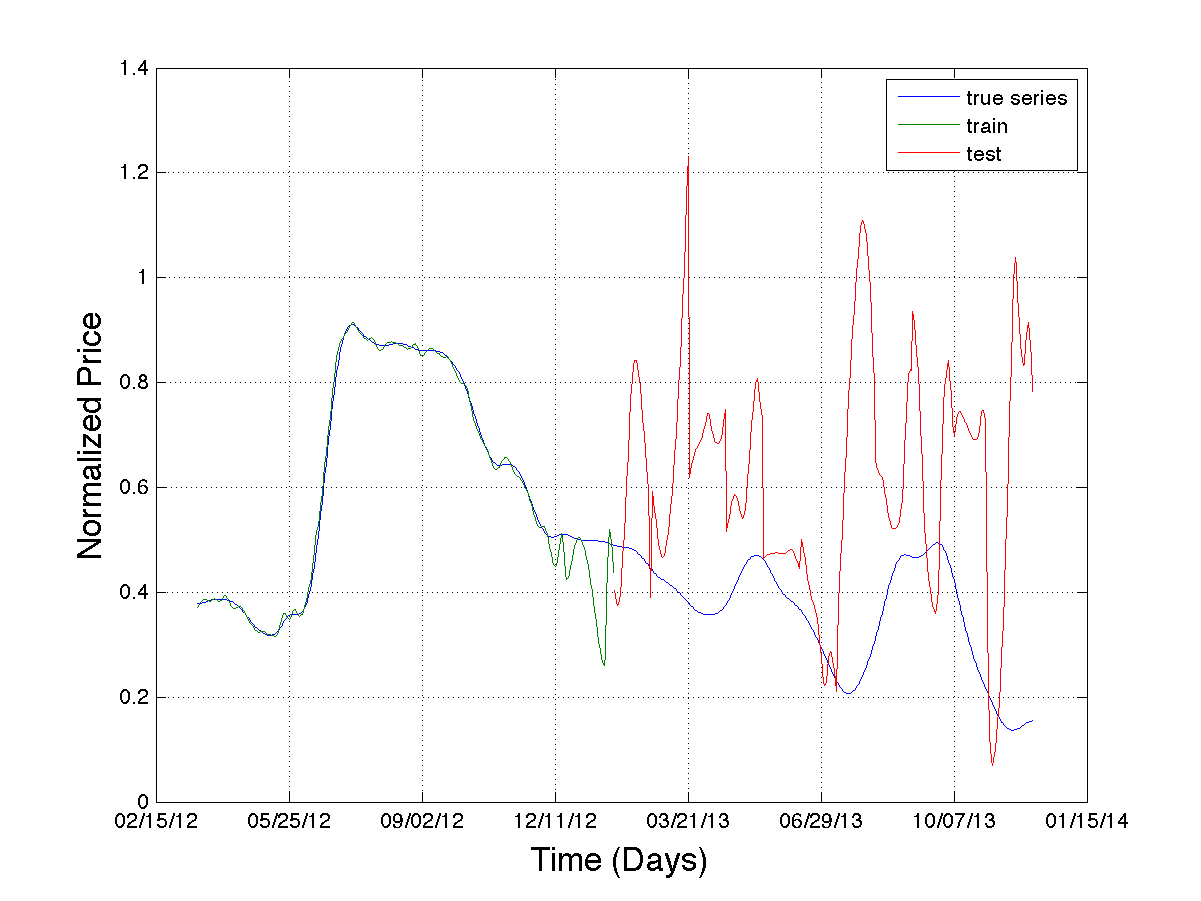
\includegraphics[width=\textwidth]{img/model/exp2/wheat/pred_1}
                \caption{1 Day Horizon Wheat - RMSE 0.3580}
                \label{fig:gull}
        \end{subfigure}%
           \begin{subfigure}[b]{0.5\textwidth}
                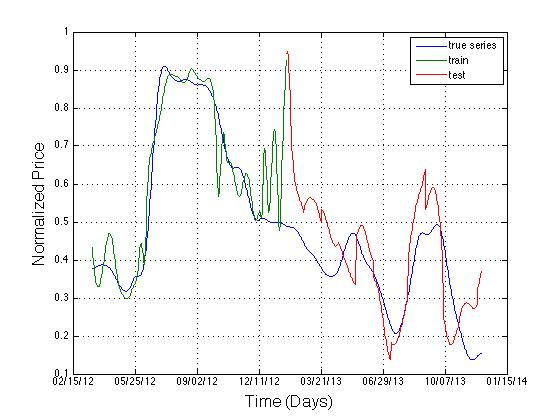
\includegraphics[width=\textwidth]{img/model/exp2_final/wheat_1}
                \caption{1 Day Horizon Wheat - RMSE 0.1083}
                \label{fig:gull}
        \end{subfigure}%
              \hfill    
        \begin{subfigure}[b]{0.5\textwidth}
                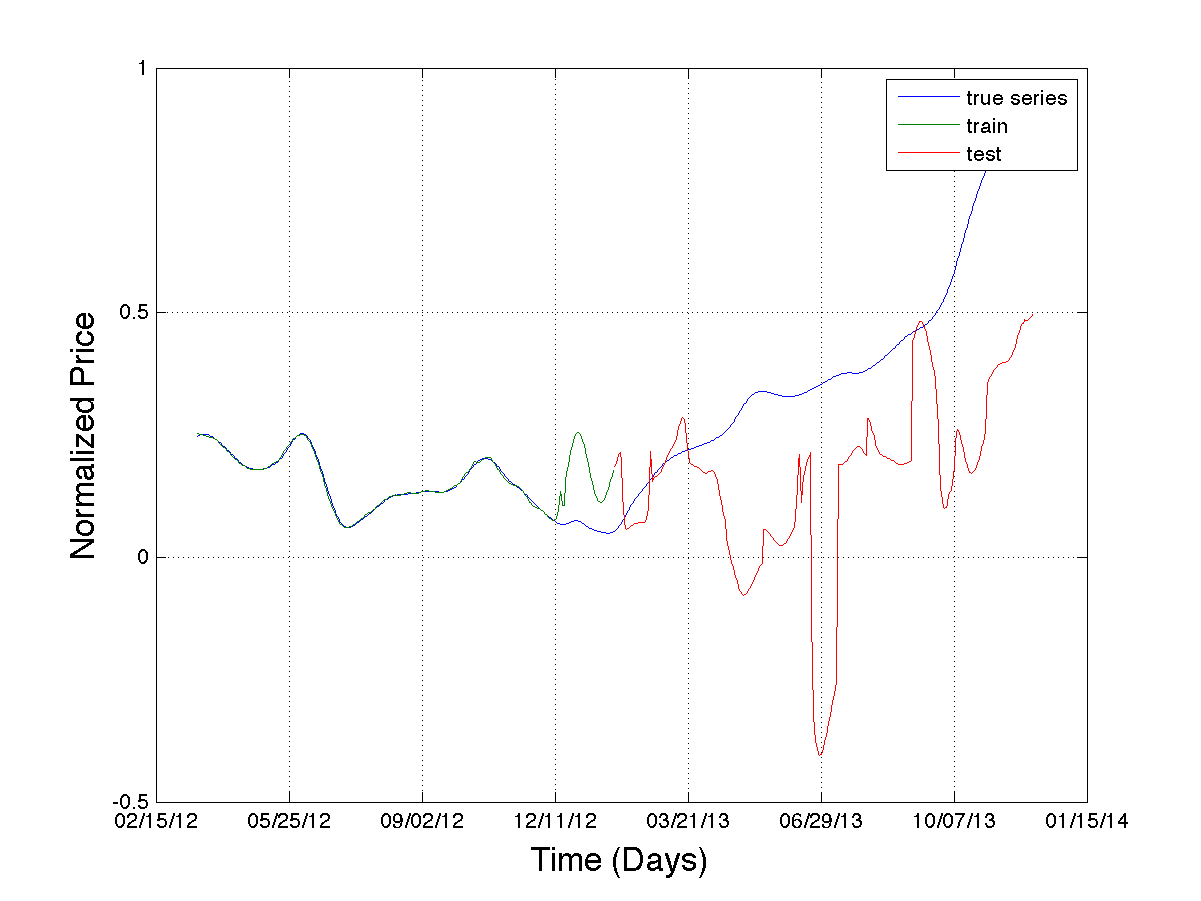
\includegraphics[width=\textwidth]{img/model/exp2/beef/pred_1}
                \caption{1 Day Horizon Beef - RMSE 0.3209  }
                \label{fig:tiger}
        \end{subfigure}%
              \begin{subfigure}[b]{0.5\textwidth}
                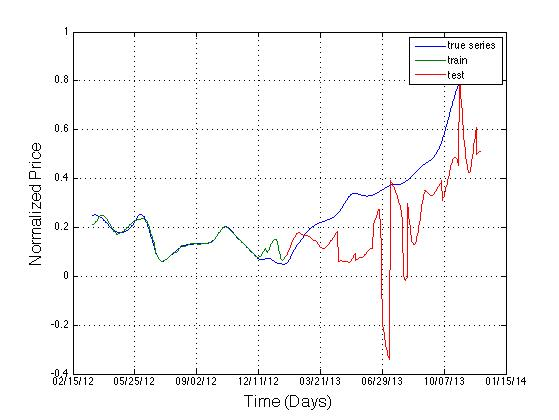
\includegraphics[width=\textwidth]{img/model/exp2_final/beef_1}
                \caption{1 Day Horizon Beef  - RMSE 0.2383 }
                \label{fig:tiger}
        \end{subfigure}%
      	 \hfill
        \begin{subfigure}[b]{0.5\textwidth}
                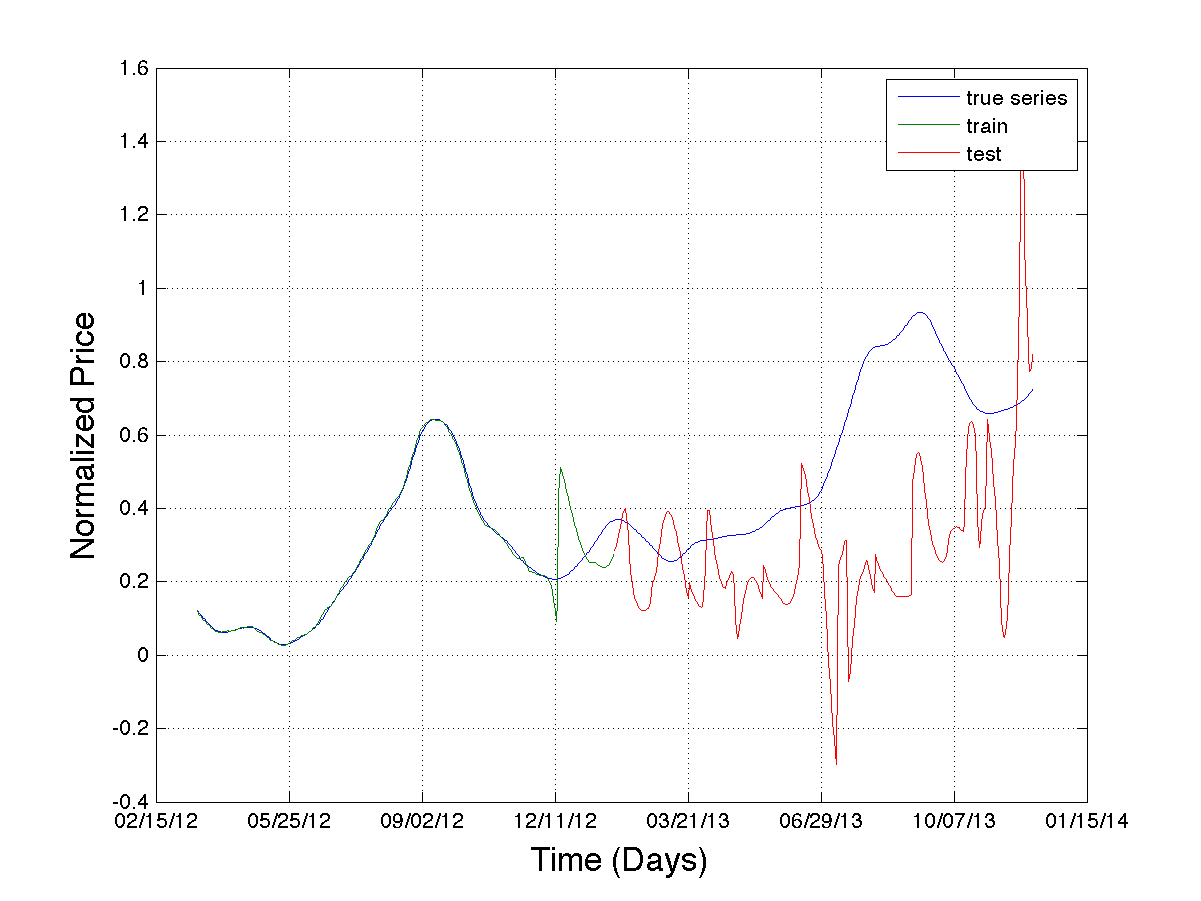
\includegraphics[width=\textwidth]{img/model/exp2/milk/pred_1}
                \caption{1 Day Horizon Milk- RMSE 0.3782}
                \label{fig:mouse}
        \end{subfigure}%
            \begin{subfigure}[b]{0.5\textwidth}
                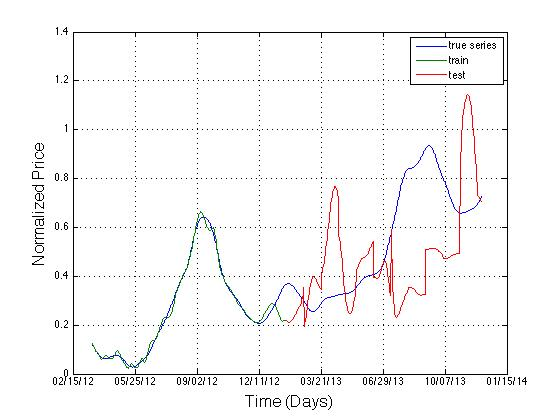
\includegraphics[width=\textwidth]{img/model/exp2_final/milk_1}
                \caption{1 Day Horizon Milk - RMSE  0.2960}
                \label{fig:mouse}
        \end{subfigure}%
    
    
        \caption{Social Media Prediction}\label{fig:comp_exp}
\end{figure}




\subsection{Combined Model}


\subsection{Feature Selection}

Combining the price and social media features we want to investigate if Relieff proposes as similar set as for the separate models or if the combined model favours a different group of input variables. Only a few features generalised well over all commodities which is why we focuses our search of finding input variables that are specific to beef, milk and wheat but generalise well over different prediction models. As in our price model, days in the intermediate past were proposed for all three commodities. The ratio varies very strongly between the commodities. Beef favours price variables where milk and wheat have a majority of social media features. We observe an interesting trend, namely that all commodities favour supply and needs feature over price and poverty which is very different to the pure social media model. We assume that the price data made the conversations about price more obsolete. 


the third sentiment ratio of poverty (SR34), 
the fith sentiment of the product (SR12), 
the fourth sentiment of the product(SR11), 
the fourth sentiment of supply (SR47)
the third sentiment of supply (SR46)
the second sentiment of supply(SR45)
the first sentiment of price (SR38)
the third sentiment of price (SR40)
the third sentiment of the category (SR22)
the fourth sentiment of needs(SR29)
the fith sentiment of needs(SR30)
the sixth sentiment of needs(SR31)
the first sentiment of the subcategory (SR15)


D24 = (75)
D25 = (76)
D26 = (77)
D27 = (78)
D28 = (79)
D29 = (80)
D30 = (81)
W1 = (82)





\begin{table}[H]
\centering
\begin{tabular}{ |p{2cm}|p{1cm}|p{1cm}|p{1cm}|p{1cm}|p{1cm}|p{1cm}|p{1cm}|p{1cm}|p{1cm}| p{1cm}|  }
\hline
$milk$ & SR38 & SR40 & SR45 & D30 & D29 &  SR34 & SR12 & SR47 & SR46 & SR11 \\
\hline
$beef$ & SR38 & D30 & D29 & D28 & D27 &  W1 & D26 & SR45 & D25 & D24 \\
\hline
$wheat$ & D30 & D29 & SR22 & SR29 & SR30 & SR31 & SR15 & SR16 & SR33 & SR14 \\
\hline
\end{tabular}
\caption{Feature Selection: Benchmark Prediction}
\label{tab:feat_mod3}
\end{table}









\subsection{Curse of of Dimensionality}

For Fuzzy interference systems there are generally three types of input space partitionings. We can classify them as grid, true and scattered portionin. We first applied grid pertaining which generates rules by enumerating all possible combinations of membership functions. However for three membership functions and x features this leads to $3^x$ possible combinations. Instead of enumerating all possible rules we used a sub clustering method to provide a fast, one pas method to take input-output training data and generate a Fuzzy Interference System. 






Data Source: 

Cattle \footnote{$https://www.quandl.com/data/OFDP/FUTURE_DA1-CME-Class-III-Milk-Futures-Continuous-Contract-1-DA1-Front-Month$}
Milk \footnote{$https://www.quandl.com/data/WSJ/MILK-Milk-Non-Fat-Dry-Chicago$}

Corn \footnote{$https://www.quandl.com/data/OFDP/FUTURE_C1-CBOT-Corn-Futures-Continuous-Contract-1-C1-Front-Month$}
Wheat \footnote{$https://www.quandl.com/data/OFDP/FUTURE_W1-CBOT-Wheat-Futures-Continuous-Contract-1-W1-Front-Month$}







Fuzzy logic based modeling techniques are appealing because of their interpretability and potential to address a broad spectrum of problems. In particular, fuzzy inference systems exhibit a combined description and prediction capability a s a consequence of their rule based structure [27, 49]

Non linear system better results in time series predictions. 

M. De Choudhury, H. Sundaram, A. John, and D. D. Seligmann, ?Can blog communication 
20
dynamics be correlated with stock market activity?,? in Proceedings of the nineteenth ACM 




$http://www.cemla.org/red/papers2002/RED_VII_CANADA-Lalonde-Zhu-Demers.pdf$ This reference showd prediction for commodities in rang of 0.06 and 0.08 for 4 days. we are within acceptable range. 


 
